%!TEX root = main.tex


\documentclass[USenglish,onecolumn]{article}
\usepackage[big]{dgruyter}

% \usepackage[utf8]{inputenc}%(only for the pdftex engine)
% \RequirePackage[no-math]{fontspec}%(only for the luatex or the xetex engine)
 
%!TEX root = main.tex


%----------------------------------------------------------------------------------------

%----------------------------------------------------------------------------------------
%	Optional Packages
%----------------------------------------------------------------------------------------
\usepackage{graphicx}
\usepackage[figuresright]{rotating}

\usepackage[font={itshape,raggedright},begintext=``,endtext="]{quoting}
\usepackage{microtype}
\usepackage[framemethod=TikZ]{mdframed}
\usepackage{multirow}
\usepackage{tabulary}
\usepackage{glossaries}
\usepackage{textcomp}
% \usepackage[]{todonotes}


\usepackage{hyperref}       % hyperlinks
\PassOptionsToPackage{hyphens}{url}
\usepackage{amsfonts}       % blackboard math symbols
\usepackage{nicefrac}       % compact symbols for 1/2, etc.

%%%%%%%%%%%%%%%%%%%%%%%%%%%%%%%%%%%%%%%%%%%%%%%%%%%%%%%%%%%%%%%%%%%%%%%%%%
% Following additional macros are required to function some 
% functions which are not available in the class used.
%%%%%%%%%%%%%%%%%%%%%%%%%%%%%%%%%%%%%%%%%%%%%%%%%%%%%%%%%%%%%%%%%%%%%%%%%%


% My packages
\usepackage{tikzit}
\input{diagrams.tikzstyles}
\usepackage[mathscr]{euscript}
\usepackage {tikz}
\usetikzlibrary {positioning}
\usetikzlibrary{shapes.misc}
\usetikzlibrary{shapes.geometric}
\usetikzlibrary{calc}
\usetikzlibrary{arrows.meta}
\usetikzlibrary{intersections}
\usepackage[intlimits,tbtags]{amsmath}
\usepackage{amsthm}
\usepackage{amssymb}

\usepackage{dsfont}
\usepackage{stmaryrd }
\usepackage{csquotes}
\usepackage{wasysym}
\usepackage[shortlabels]{enumitem}
\usepackage{bm}
\usepackage{isomath}
\usepackage{mathtools}
\usepackage{algpseudocode}
\usepackage{algorithm}
\usepackage{multirow}

\usepackage{mathtools}
\mathtoolsset{showonlyrefs}


\hyphenation{un-con-found-ed-ness-like}
\hyphenation{un-con-found-ed-ness}
%----------------------------------------------------------------------------------------
%	MATHS SETTINGS
%----------------------------------------------------------------------------------------


\makeatletter
\newcommand{\newreptheorem}[2]
  {\newtheorem*{rep@#1}{\rep@title}\newenvironment{rep#1}[1]
  {\def\rep@title{#2 \ref*{##1}}\begin{rep@#1}}{\end{rep@#1}}}
\makeatother

\theoremstyle{plain}
\newtheorem{theorem}{Theorem}[section]
\newtheorem{corollary}[theorem]{Corollary}
\newtheorem{lemma}[theorem]{Lemma}
\newtheorem{proposition}[theorem]{Proposition}
\newreptheorem{theorem}{Theorem}
\newreptheorem{lemma}{Lemma}
\newreptheorem{definition}{Definition}

\newtheorem{innercustomthm}{Theorem}
\newenvironment{customthm}[1]
  {\renewcommand\theinnercustomthm{#1}\innercustomthm}
  {\endinnercustomthm}

\theoremstyle{definition}
\newtheorem{definition}[theorem]{Definition}
\newtheorem{example}[theorem]{Example}
\newtheorem{notation}[theorem]{Notation}


% \DeclareMathAlphabet{\mathsfit}{T1}{\sfdefault}{\mddefault}{\sldefault}

\newcommand{\CI}{\mathrel{\text{\scalebox{1.07}{$\perp\mkern-10mu\perp$}}}}
\newcommand{\CII}{\mathrel{\text{\scalebox{1.07}{$\perp\mkern-10mu\perp\mkern-10mu\perp$}}}}
\newcommand{\RV}[1]{\ensuremath{\mathsf{#1}}}
\newcommand{\node}[1]{\ensuremath{\mathsfit{#1}}}
\newcommand{\graph}[1]{\ensuremath{\mathsfbfit{#1}}}
\newcommand{\URV}[1]{\ensuremath{\underline{\RV{#1}}}}
\newcommand{\PA}[2]{\ensuremath{\text{Pa}_{#1}(#2)}}
\newcommand{\ND}[2]{\ensuremath{\text{ND}_{#1}(#2)}}
\newcommand{\CH}[2]{\ensuremath{\text{Ch}_{#1}(#2)}}
\newcommand{\DE}[2]{\ensuremath{\text{De}_{#1}(#2)}}
\newcommand{\ID}[1]{\ensuremath{\text{Id}_{#1}}}
\newcommand{\utimes}{\ensuremath{\underline{\otimes}}}
\newcommand{\prob}[1]{\ensuremath{\mathbb{#1}}}
\newcommand{\disint}[1]{\ensuremath{\overline{\prob{#1}}}}
\newcommand{\kernel}[1]{\ensuremath{\mathbb{#1}}}
\newcommand{\model}[1]{\ensuremath{\mathbb{#1}}}
\newcommand{\diagram}[1]{\ensuremath{\mathscr{#1}}}
\newcommand{\sigalg}[1]{\ensuremath{\mathcal{#1}}}
\newcommand{\vecRV}[1]{\ensuremath{\mathsfbfit{#1}}}
\newcommand{\vecVal}[1]{\ensuremath{\mathbf{#1}}}
\newcommand{\prodSet}[1]{\ensuremath{\mathbf{#1}}}
\newcommand{\indx}[1]{\ensuremath{\mathcal{#1}}}
\newcommand{\nod}[1]{\ensuremath{\mathsfit{#1}}}
\newcommand{\kto}{\ensuremath{\rightarrowtriangle}}
\newcommand{\proc}[1]{\ensuremath{\mathscr{#1}}}
\newcommand{\yields}{\ensuremath{\bowtie}}
\newcommand{\submodel}{\ensuremath{\sqsubset}}
\newcommand{\seedo}[5]{\ensuremath{\model{#1}^{\RV{#3}|\RV{#2}\square\RV{#5}|\RV{#4}}}}
\newcommand{\rseedo}[6]{\ensuremath{\model{#1}^{\RV{#3}|\RV{#2}\framebox{#6}\RV{#5}|\RV{#4}}}}
\newcommand{\set}{\ensuremath{\bowtie}}
\newcommand{\cprod}{\ensuremath{\odot}}
\newcommand{\bigcprod}{\ensuremath{\bigodot}}
\newcommand{\combprod}{\ensuremath{\underline{\cprod}}}
\newcommand{\combbreak}{\ensuremath{\wr}}
\newcommand{\combgap}{\ensuremath{\shortleftarrow}}
\newcommand{\bigcombprod}{\ensuremath{\underline{\bigcprod}}}
\newcommand{\varlessthan}{\ensuremath{\preccurlyeq}}
\algnewcommand\algorithmicassert{\texttt{assert}}
\algnewcommand\Assert[1]{\State \algorithmicassert(#1)}%



\providecommand\longrightarrowRHD{\relbar\joinrel\relbar\joinrel\mathrel\RHD}
\providecommand\longleftarrowRHD{\mathrel\LHD\joinrel\relbar\joinrel\relbar}

\makeatletter
\newcommand*\bigcdot{\mathpalette\bigcdot@{.5}}
\newcommand*\bigcdot@[2]{\mathbin{\vcenter{\hbox{\scalebox{#2}{$\m@th#1\bullet$}}}}}
\makeatother

\tikzset{
    triangle/.style = {regular polygon, regular polygon sides=3 },
    node rotated/.style = {rotate=90},
    border rotated/.style = {shape border rotate=90},
    dist/.style = {triangle,draw,border rotated, inner sep=0pt},
    smalldist/.style = {triangle,draw,border rotated},
    kernel/.style={rectangle,draw,inner sep = 2pt},
    expectation/.style = {triangle,draw,inner sep=0pt,shape border rotate=270},
    copymap/.style = {circle,fill,inner sep=1pt}}

\newcommand\DCI{
    \begin{tikzpicture}[scale=0.35]
    \draw[->] (1,0) -- (0,0);
    \draw (0.6,0) -- (0.6,0.75);
    \draw (0.4,0) -- (0.4,0.75);
    \end{tikzpicture}
}

\newcommand\splitter[1]{%
\begin{tikzpicture}[scale=#1]
\draw (0,-1) -- (0,0);
\draw (0,0) to [bend right] (1,1);
\draw (0,0) to [bend left] (-1,1);
\end{tikzpicture}
}

\newcommand\stopper[1]{%
\begin{tikzpicture}[scale=#1]
\draw[-{Rays [n=8]}] (0,-1) -- (0,0);
\end{tikzpicture}
}

\newcommand\swap[1]{%
\begin{tikzpicture}[scale=#1]
\draw (0,0) to [out=90, in=270] (0.5,1);
\draw (0.5,0) to [out=90,in=270] (0,1);
\end{tikzpicture}
}

\newcommand\source[1]{%
\begin{tikzpicture}[scale=#1]
\path (0,0) node[prob,fill=gray] (P) {};
\draw (P) -- ($(P.east) + (1,0)$);
\end{tikzpicture}
}

\DeclareMathOperator*{\argmax}{arg\,max}
\DeclareMathOperator*{\argmin}{arg\,min}
\DeclareMathOperator*{\arginf}{arg\,inf}
\DeclareMathOperator*{\argsup}{arg\,sup}

\newcommand{\cheng}[1]{ {\color{purple}[{\bf Cheng:~{#1}}]} }


%----------------------------------------------------------------------------------------
%	BOX SETTINGS
%----------------------------------------------------------------------------------------
% from https://texblog.org/2015/09/30/fancy-boxes-for-theorem-lemma-and-proof-with-mdframed/

%----------------------------------------------------------------------------------------
%	MARGIN SETTINGS
%----------------------------------------------------------------------------------------



  
\begin{document}
 

  \articletype{Research Article{\hfill}Open Access}

  \author*[1]{David Johnston}

  \author[2]{Cheng Soon Ong}

  \author[3]{Robert C. Williamson}

  \affil[1]{Australian National University; E-mail: davidoj@fastmail.com.au}

  \affil[2]{Data61; E-mail; chengsoon.ong@anu.edu.au}

  \affil[3]{Universität Tübingen; Email: bob.williamson@uni-tuebingen.de}

  \title{\huge Causal Inference Without Interventions}

  \runningtitle{Inference Without Interventions}

  %\subtitle{...}

  \begin{abstract}
{Valid causal inferences from diverse data are a tantalizing but elusive prospect. Assumptions are necessary to make any inferences, and these assumptions cannot all be washed out by sufficiently large datasets, and they consequently require strong prior support. We argue that structural interventions in particular frequently embody assumptions not entailed by prior knowledge or by the given data. A key role of structural interventions is to identify fixed relationships that are shared by data arising from observation and by data arising from the consequences of a decision. We show that structural interventions are not required to analyse assumptions of fixed relationships like this. Our starting point is is to ground causal models in the problem of making good decisions, and our first result is an equivalence between decision models with "sequences of identical conditionals" and decision models that feature a symmetry we call "IO contractibility". This can be seen as a generalisation of De Finetti's work on exchangeability, itself an attempt to justify the conventional but seemingly mysterious assumption of sequences featuring a "shared but unknown probability distribution". We argue that IO contractibility is often an unreasonable assumption. Our second result is that IO contractibility may be implied by a combination of an observed conditional independence and a weaker assumption based on the principle of ``precedent'', which requires that everything that might be done has already been done before in some way and has been seen to work. We discuss a connection between this latter result and constraint based causal discovery.}
\end{abstract}
  \keywords{causal inference, decision theory}
   \classification[MSC]{62C99} % Decision theory - other (62C05 also maybe?)
 % \communicated{...}
 % \dedication{...}

  \journalname{Journal of Causal Inference}
\DOI{DOI}
  \startpage{1}
  \received{..}
  \revised{..}
  \accepted{..}

  \journalyear{2022}
  \journalvolume{1}
%  \journalissue{1}
 

\maketitle
\section{Introduction}

Judea Pearl's causal hierarchy distinguishes between three types of problems: prediction problems, intervention problems, and counterfactual problems \citep{pearl_book_2018}. Modelling an intervention problem requires a different kind of knowledge than that required for modelling predictions, and modelling a counterfactual problem requires a different kind of knowledge than that needed for modelling intervention problems.

While we think that Pearl's hierarchy offers an important insight into the differences between causal inference and classical statistics, we feel the terminology of interventions is confusing. In Pearl's theory, \emph{structural interventions} are used to model what he describes as intervention problems. Structural interventions are operations that transform a probability distribution according to a \emph{graphical causal model}. However, ``intervention problems'' refer to a broad class of problems that ask questions like ``what will happen if I do this? what will happen if I do something else instead?'' -- problems that we frequently encounter whether or not we make use of graphical causal models. This kind of problem often comes up we want to make a decision; given various options and some idea of the outcomes we would like to achieve, we want to know what the likely consequences of each option are.

As the terminology suggests, structural interventions and graphical causal models are often used as a tool for modelling the consequences of different options (that is, ``structural interventional models'' are used to model ``intervention problems'' broadly understood). However, using structural interventions to model the consequences of different options poses a conundrum. Our decision maker has some set of options $C$ to consider, and selecting an option $\alpha$ from this set is their decision problem. Given a dataset, they may attempt to infer causal relationships using causal discovery, or to estimate certain structural intervention-based effects of interest from the data along with whatever causal assumptions they supplied at the outset. Typically, whatever learning or estimation takes place, it does \emph{not} include an attempt to learn a correspondence between each of their options $\alpha$ and a structural intervention -- this correspondence is usually assumed to be prior knowledge. However, such a correspondence seemingly goes beyond the kind of prior knowledge a decision maker is likely to have.

The most common kind of structural intervention is known as a \emph{perfect} or \emph{hard} intervention. A perfect intervention is often denoted with the symbol $\mathrm{do}(\RV{X}=x)$. Given a probability distribution $\prob{P}$, a variable $\RV{X}$ and a causal graphical model $\mathcal{G}$ which, among other things, specifies a set of \emph{causal parents} $\mathrm{Pa}(\RV{X})$ of $\RV{X}$, the intervention $\mathrm{do}(\RV{X}=x)$ yields a new probability distribution $\prob{P}'$ such that the conditional probability $\prob{P}^{\prime \RV{X}|\mathrm{Pa}(\RV{X})}$ becomes the function $\cdot \mapsto \delta_x$, while all other conditional distributions of a ``child'' conditional on its ``parents'' according to $\mathcal{G}$ match their counterparts in $\prob{P}$ \citep[Sec. 1.3.1]{pearl_causality:_2009}

Thus identifying a perfect intervention $\mathrm{do}(\RV{X}=x)$ with an option $\alpha$ embodies a collection of assumptions -- first, it embodies the assumption that selecting the option $\alpha$ will force future observations of the variable $\RV{X}$ to take the value $x$. This information may sometimes (though not always) be available to decision makers. However, the identification of options with perfect interventions also embodies the assumption that selecting the option $\alpha$ will leave all ``parental conditionals'' with respect to $\mathcal{G}$ unchanged with the exception of $\prob{P}^{\prime \RV{X}|\mathrm{Pa}(\RV{X})}$. It's harder to see how a decision maker could know this.

It's possible that the decision maker might choose the graph $\mathcal{G}$ carefully just so that these additional conditions hold. If so, the decision maker must know exactly which conditionals are invariant a priori, and the graphical model $\mathcal{G}$ is merely a convenient shorthand for representing this knowledge. Typically a decision maker's prior knowledge will not be so extensive. Furthermore, adapting the graph to the set of options under consideration conflicts with normal practice in causal discovery where the learned graph does not depend on the options under consideration. Common measures of success in causal discovery are the structural intervention distance \citep{peters_structural_2015} and the structural hamming distance, neither of which depend on the options under consideration \citep{scherrer_learning_2022, toth_active_2022, brouillard_differentiable_2020, forre_constraint-based_2018, chickering_optimal_2003}. The idea that the relationships captured by a causal graph are independent of the options under consideration is also defended in \citet{pearl_does_2018}. 

% I don't know why these citations don't work
% \citep{ngGraphAutoencoderApproach2019 ,zhengDAGsNOTEARS2018, spirtes_causation_1993}

On the other hand, it is not obvious to us how a decision maker could know a priori that their options correspond to perfect interventions on some unknown ``objectively correct'' graphical model. We can also raise a concrete arguments against the notion that actions known in advance to affect a certain variable can typically be assumed to be interventions on that variable: there are multiple different ways to influence many variables we are interested in measuring and they cannot all be perfect interventions. \citet{hernan_does_2008,noauthor_does_2016} considers the example of different options that are known a priori to affect a person's body mass index, including diet plans, gastric bypass surgery and limb removal. These will all plausibly affect an individual's risk of death differently, and so they cannot all be modeled by the same intervention on body mass index. Further, it seems to us (as well as other authors in this exchange \citep{pearl_does_2018,hernanInvitedCommentaryCausal2009,shahar_association_2009}) that none of these options stand out as a strong candidate to be identified with a perfect intervention on body mass index. The difficulty is twofold: first, we don't know what makes the ``true graph'' true, and as a result it is not clear how to decide which option if any should be be identified with perfect interventions on this graph. Second, it is not even obvious which action represents the ``canonical'' way to alter a person's body mass index so it is not clear how we could verify that any procedure for learning a causal graph actually yields the correct interventions as a result.

Hernán argues that limb removal can be dismissed as an option because it is not interesting from a scientific or public health standpoint. While this is a reasonable contention, demanding that a causal graph correctly represent options that are interesting from a scientific or public health standpoint is a version of the strategy of of choosing the graph so that the options of interest are correctly represented, which as we've mentioned is not the standard practice in causal discovery.

Perhaps in recognition of the fact that many actions are not modeled by perfect interventions, there is a diverse array of structural interventions that can be found in the literature: a non-exhaustive review reveals perfect interventions or ``hard'' interventions \citep[ch. ~1]{pearl_causality:_2009,hauser_characterization_2012}, soft interventions \citep{correa_calculus_2020,eberhardt_interventions_2007}, general or fat-hand interventions \citep{eberhardt_interventions_2007,yang_characterizing_2018,glymour_evaluating_2017} and general interventions with unknown targets \citep{brouillard_differentiable_2020}. However, as in the case of perfect interventions, none of these generalised families of structural interventions make provisions for learning the option-intervention correspondence.

Notwithstanding our criticisms, the assumptions of invariant parental conditional distributions made by structural interventional models play a very important role in the interpretation of graphical causal models. If a decision maker wants to learn from some observed data so as to make a better decision, then these assumptions tell them what the observational data and the consequences of their decisions will have in common: the parental conditional distributions. In this paper, we show that structural interventions are not the \emph{only} way of analysing assumptions of this type.

We investigate whether certain assumptions of symmetry are a viable alternative to structured interventions for this task of using features of observations to forecast consequences of different options. In particular, we are interested in assumptions about the future being like the past. In probability models, an assumption of this type is the assumption of \emph{exchangeability}, which holds that reordering a sequence of observed variables leaves a forecaster with exactly the same prediction problem. This assumption cannot be applied as-is to decision models because, in decision problems, future events are affected by the choices made by the decision maker and therefore cannot be in all respects similar to previously observed events.

We investigate two different assumptions inspired by the idea that ``the future is in some sense like the past''. First, we introduce the idea of \emph{input-output contractibility} (IO contractibility), which can be viewed as a generalisation of exchangeability to decision models. In particular, we show a theorem analogous to De Finetti's famous representation \citep{de_finetti_foresight_1992} theorem holds; IO contractibility is equivalent to the assumption that there is a shared but unknown input-output map for both the observations and the consequences of a decision maker's choices (Theorem \ref{th:ciid_rep_kernel}). Unlike exchangeability, however, IO contractibility is not an appealing assumption in many data-driven decision problems.

We subsequently explore the general principle of \emph{precedent}, which holds that everything a decision maker can do has been done before.  We show that under the assumption of \emph{diverse precedent}, based on the principle of precedent, conditional independences imply the stronger conclusion of IO contractibility and with it the possibility of estimating an input-output conditional distribution from the given observational data (Theorem \ref{th:latent_to_observable}). A key assumption of Theorem \ref{th:latent_to_observable} is that the posterior of the parametrisation of a certain conditional distribution is dominated by the uniform measure. We discuss, speculatively, how this assumption may be related to causal structures, noting similar assumptions that appear in \citet{meek_strong_1995} and \citet{janzingCausalVersionsMaximum2021}.

Section \ref{sec:tech_prereq} introduces the formalism of decision models. These differ from probability models in that they are a map from a set of options to distributions over consequences. We make use of the notion of \emph{extended conditional independence} introduced by \citet{constantinou_extended_2017}, which is a notion of conditional independence relevant to decision models. Section \ref{sec:evaluating_decisions} introduces the idea of shared conditionally independent and identical responses, and shows that this is equivalent to the assumption of input-output in Theorem \ref{th:ciid_rep_kernel}. Section \ref{sec:precedent} explains the assumption of precedent and proves Theorem \ref{th:latent_to_observable} and discusses the interpretation of this assumption and its connection to structural causal models.

\subsection{Previous work on symmetries in causal inference}\label{sec:prev_work}

The approach that we take assumes that decision making is the fundamental problem that requires causal inference. This assumption motivates the formalism of ``decision models'' that we use to investigate the questions raised here. The broad idea of starting with the options available to a decision maker rather than starting with some foundational notion of causation is often called the \emph{decision theoretic approach to causal inference} \citep{heckerman_decision-theoretic_1995,dawid_decision-theoretic_2012,dawid_decision-theoretic_2020}. \citet{lattimore_causal_2019,lattimore_replacing_2019} also document an approach to causal modelling that demands explicit consideration of the set of interventions, and is arguably an example of the decision theoretic approach.

\citet{lindley_role_1981} discussed sequences of exchangeable observations along with ``one more observation''. Lindley mentioned the application of this model to questions of causation, but did not explore this deeply due to the perceived difficulty of finding a satisfactory definition of causation. \citet{rubin_causal_2005, imbens_causal_2015} made use of the assumption of models with exchangeable potential outcomes to prove several identification results. \citet{saarela_role_2020}, used graphical causal models to propose \emph{conditional exchangeability}, defined as the exchangeability of the non-intervened causal parents of a target variable under intervention on its remaining parents. Sareela et. al. suggested that this could be interpreted as a symmetry of an experiment involving administering treatments to patients with respect to exchanging the patients in the experiment. \citet{hernan_estimating_2006,hernan_beyond_2012,greenland_identifiability_1986,banerjee_chapter_2017,dawid_decision-theoretic_2020} all discuss similar experimental symmetries. These symmetries are reminiscent of \emph{exchange commutativity} discussed here. They're not identical, however -- exchange commutativity can be justified by the equivalence of certain prediction problems that arise from a single experiment, instead of an equivalence of different experiments that arise from, for example, interchanging experimental subjects.

A different kind of regularity of causal models is given by the stable unit treatment distribution assumption (SUTDA) in \citet{dawid_decision-theoretic_2020} and the stable unit treatment value assumption (SUTVA) in \citep{rubin_causal_2005}. This regularity is similar to the condition of \emph{locality} introduced here.

Theorem \ref{th:latent_to_observable} was inspired by the idea of \emph{causal inference by invariant prediction} \citep{peters_causal_2016}. While both the assumptions and the conclusions drawn in that work differ from the assumptions and conclusion of Theorem \ref{th:latent_to_observable}, both proceed from an idea that can be roughly described as ``things I can do have been done before'' and both look for variable pairs $\RV{X}$ and $\RV{Y}$ such that the distribution of $\RV{Y}$ given $\RV{X}$ doesn't change after actions are taken. Finally, the variable described in that work as ``the environment'' is similar to the variable $\RV{Z}$ in Theorem \ref{th:latent_to_observable} in that neither variable needs to be IID, and both variables are only necessarily of interest in the observation set, and need not be of any interest for the consequences of actions.

%!TEX root = main.tex


\section{Technical Prerequisites}\label{sec:tech_prereq}

Our approach to causal inference is based on probability theory. Many results and conventions will be familiar to readers, and these are collected in Section \ref{sec:standard_prob}. Because decision models are stochastic functions rather than probability measures (Section \ref{sec:probability_sets}), we make use a generalisation of conditional independence called \emph{extended conditional independence}, explained in Section \ref{sec:eci}.

\subsection{Probability Theory}\label{sec:standard_prob}

\subsubsection{Measurable spaces}

\begin{definition}[Sigma algebra]
Given a set $A$, a $\sigma$-algebra $\mathcal{A}$ is a collection of subsets of $A$ where
\begin{itemize}
	\item $A\in \mathcal{A}$ and $\emptyset\in \mathcal{A}$
	\item $B\in \mathcal{A}\implies B^{\complement}\in\mathcal{A}$
	\item $\mathcal{A}$ is closed under countable unions: For any countable collection $\{B_i|i\in Z\subset \mathbb{N}\}$ of elements of $\mathcal{A}$, $\cup_{i\in Z}B_i\in \mathcal{A}$ 
\end{itemize}
\end{definition}

\begin{definition}[Measurable space]
A measurable space $(A,\mathcal{A})$ is a set $A$ along with a $\sigma$-algebra $\mathcal{A}$.
\end{definition}

\begin{definition}[Sigma algebra generated by a set]
Given a set $A$ and an arbitrary collection of subsets $U\supset\mathscr{P}(A)$, the $\sigma$-algebra generated by $U$, $\sigma(U)$, is the smallest $\sigma$-algebra containing $U$.
\end{definition}

\paragraph{Common $\sigma$ algebras}

For any $A$, $\{\emptyset,A\}$ is a $\sigma$-algebra. In particular, it is the only sigma algebra for any one element set $\{*\}$.

For countable $A$, the power set $\mathscr{P}(A)$ is known as the discrete $\sigma$-algebra.

Given $A$ and a collection of subsets of $B\subset\mathscr{P}(A)$, $\sigma(B)$ is the smallest $\sigma$-algebra containing all the elements of $B$. 

If $A$ is a topological space with open sets $T$, $\mathcal{B}(\mathbb{R}):=\sigma(T)$ is the \emph{Borel $\sigma$-algebra} on $A$.

If $A$ is a separable, completely metrizable topological space, then $(A,\mathcal{B}(A))$ is a \emph{standard measurable set}. All standard measurable sets are isomorphic to either $(\mathbb{R},B(\mathbb{R}))$ or $(C,\mathscr{P}(C))$ for denumerable $C$ \citep[Chap. 1]{cinlar_probability_2011}.

\subsubsection{Probability measures and Markov kernels}

\begin{definition}[Probability measure]\label{def:prob_meas}
Given a measurable space $(E,\sigalg{E})$, a map $\mu:\sigalg{E}\to [0,1]$ is a \emph{probability measure} if
\begin{itemize}
	\item $\mu(E)=1$, $\mu(\emptyset)=0$
	\item Given countable collection $\{A_i\}\subset\mathscr{E}$, $\mu(\cup_{i} A_i) = \sum_i \mu(A_i)$
\end{itemize}
\end{definition}

\begin{definition}[Set of all probability measures]\label{no:prob_meas_set}
The set of all probability measures on $(E,\sigalg{E})$ is written $\Delta(E)$. We equip $\Delta(E)$ with the coarsest $\sigma$-algebra such that the evaluation maps $\eta_B:\nu\mapsto \nu(B)$ are measurable for all $B\in \sigalg{F}$.
\end{definition}

\begin{definition}[Probability space]
A probability space is a triple $(\mu,E,\sigalg{E})$ consisting of a probability measure and a measurable space.
\end{definition}

\begin{definition}[Markov kernel]\label{def:markov_kern}
Given measurable spaces $(E,\sigalg{E})$ and $(F,\sigalg{F})$, a \emph{Markov kernel} or \emph{stochastic function} is a map $\kernel{M}:E\times\sigalg{F}\to [0,1]$ such that
\begin{itemize}
	\item The map $\kernel{M}(A|\cdot):x\mapsto \kernel{M}(A|x)$ is $\sigalg{E}$-measurable for all $A\in \sigalg{F}$
	\item The map $\kernel{M}(\cdot|x):A\mapsto \kernel{M}(A|x)$ is a probability measure on $(F,\sigalg{F})$ for all $x\in E$
\end{itemize}
\end{definition}

\begin{notation}[Signature of a Markov kernel]
Given measurable spaces $(E,\sigalg{E})$ and $(F,\sigalg{F})$ and $\kernel{M}:E\times\sigalg{F}\to [0,1]$, we write the signature of $\kernel{M}:E\kto F$, read ``$\kernel{M}$ maps from $E$ to probability measures on $F$''.
\end{notation}

\begin{definition}[Deterministic Markov kernel]
A \emph{deterministic} Markov kernel $\kernel{A}:E\to \Delta(\mathcal{F})$ is a kernel such that $\kernel{A}_x(B)\in\{0,1\}$ for all $x\in E$, $B\in\mathcal{F}$.
\end{definition}

\paragraph{Common probability measures and Markov kernels}

\begin{definition}[Dirac measure]\label{def:dirac_meas}
The \emph{Dirac measure} $\delta_x\in \Delta(X)$ is a probability measure such that $\delta_x(A)=\llbracket x\in A \rrbracket$
\end{definition}

\begin{definition}[Markov kernel associated with a function]\label{def:mkern_func}
Given measurable $f:(X,\sigalg{X})\to (Y,\sigalg{Y})$, $\kernel{F}_f:X\kto Y$ is the Markov kernel given by $x\mapsto \delta_{f(x)}$
\end{definition}

\begin{definition}[Markov kernel associated with a probability measure]
Given $(X,\sigalg{X})$, a one-element measurable space $(\{*\},\{\{*\},\emptyset\})$ and a probability measure $\mu\in \Delta(X)$, the associated Markov kernel $\kernel{Q}_\mu:\{*\}\kto X$ is the unique Markov kernel $*\mapsto \mu$
\end{definition}

\subsubsection{Variables, conditionals and marginals}

\begin{definition}[Random variable]\label{def:variable}
Given a measurable space $(\Omega,\sigalg{F})$, which we refer to as a \emph{sample space}, and a measurable space of values $(X,\sigalg{X})$, an \emph{$X$-valued random variable on $\Omega$} is a measurable function $\RV{X}:(\Omega,\sigalg{F})\to (X,\sigalg{X})$.
\end{definition}

A sequence of random variables is also a random variable.

\begin{definition}[Sequence of variables]\label{def:seqvar}
Given a sample space $(\Omega,\sigalg{F})$ and two random variables $\RV{X}:(\Omega,\sigalg{F})\to (X,\sigalg{X})$, $\RV{Y}:(\Omega,\sigalg{F})\to (Y,\sigalg{Y})$, $(\RV{X},\RV{Y}):\Omega\to X\times Y$ is the random variable $\omega\mapsto (\RV{X}(\omega),\RV{Y}(\omega))$.
\end{definition}

We define a partial order on random variables such that $\RV{Y}$ is higher than $\RV{X}$ if $\RV{X}$ is given by application of a function to $\RV{Y}$. For example, $\RV{Y}\varlessthan (\RV{W},\RV{Y})$ as $\RV{Y}$ can be obtained by composing a projection with $(\RV{W},\RV{Y})$.

\begin{definition}[Random variables determined by another random variable]\label{def:variable_po}
Given a sample space $(\Omega,\sigalg{F})$ and variables $\RV{X}:\Omega\to X$, $\RV{Y}:\Omega\to Y$, $\RV{X}\varlessthan \RV{Y}$ if there is some $f:Y\to X$ such that $\RV{X}=f\circ \RV{Y}$.
\end{definition}

We use superscripts to specify marginal and conditional distributions, as subscrips (which are a somewhat more common notation) are reserved for specifying options in decision models (Section \ref{sec:probability_sets}).

\begin{definition}[Marginal distribution]\label{def:pushforward}
Given a probability space $(\mu,\Omega,\sigalg{F})$ and a variable $\RV{X}:\Omega\to (X,\sigalg{X})$, the \emph{marginal distribution} of $\RV{X}$ with respect to $\mu$, $\mu^{\RV{X}}:\sigalg{X}\to [0,1]$ by $\mu^{\RV{X}}(A):=\mu(\RV{X}^{-1}(A))$ for any $A\in \sigalg{X}$.
\end{definition}

\begin{definition}[Conditional distribution]\label{def:disint}
Given a probability space $(\mu,\Omega,\sigalg{F})$ and variables $\RV{X}:\Omega\to X$, $\RV{Y}:\Omega\to Y$, the \emph{conditional distribution} of $\RV{Y}$ given $\RV{X}$ is any Markov kernel $\mu^{\RV{Y}|\RV{X}}:X\kto Y$ such that
\begin{align}
	\mu^{\RV{XY}}(A\times B)&=\int_{A} \mu^{\RV{Y}|\RV{X}}(B|x) \mathrm{d}\mu^{\RV{X}}(x) &\forall A\in \sigalg{X}, B\in \sigalg{Y}
\end{align}
\end{definition}

\begin{definition}[Trivial variable]\label{no:single_valued}
We let $*$ stand for any single-valued variable $*:\Omega\to \{*\}$.
\end{definition}

% \subsubsection{Markov kernel product notation}\label{ssec:product_notation}

% Three pairwise \emph{product} operations involving Markov kernels can be defined: measure-kernel products, kernel-kernel products and kernel-function products. These are analagous to row vector-matrix products, matrix-matrix products and matrix-column vector products respectively.

% \begin{definition}[Measure-kernel product]
% Given $\mu\in \Delta(\mathcal{X})$ and $\kernel{M}:X\kto Y$, the \emph{measure-kernel product} $\mu\kernel{M}\in \Delta(Y)$ is given by
% \begin{align}
% \mu\kernel{M} (A) := \int_X \kernel{M}(A|x) \mu(\mathrm{d}x)
% \end{align}
% for all $A\in \sigalg{Y}$.
% \end{definition}

% \begin{definition}[Kernel-kernel product]\label{def:kproduct}
% Given $\kernel{M}:X\kto Y$ and $\kernel{N}:Y\kto Z$, the \emph{kernel-kernel product} $\kernel{M}\kernel{N}:X\kto Z$ is given by
% \begin{align}
% \kernel{MN} (A|x) := \int_Y \kernel{N}(A|x) \kernel{M}(\mathrm{d}y|x)
% \end{align}
% for all $A\in \sigalg{Z}$, $x\in X$.
% \end{definition}

% \begin{definition}[Kernel-function product]
% Given $\kernel{M}:X\kto Y$ and $f:Y\to Z$, the \emph{kernel-function product} $\kernel{M}f:X\to Z$ is given by
% \begin{align}
% \kernel{M}f (x) := \int_Y f(y)\kernel{N}(\mathrm{d}y|x)
% \end{align}
% for all $x\in X$.
% \end{definition}

% \begin{definition}[Tensor product]
% Given $\kernel{M}:X\kto Y$ and $\kernel{L}:W\kto Z$, the tensor product $\kernel{M}\otimes\kernel{N}:X\times W\kto Y\times Z$ is given by
% \begin{align}
% 	(\kernel{M}\otimes\kernel{L})(A\times B|x,w):=\kernel{M}(A|x)\kernel{L}(B|w)
% \end{align}
% For all $x\in X$, $w\in W$, $A\in \sigalg{Y}$ and $B\in \sigalg{Z}$.
% \end{definition}

% All products are associative \citep[Chapter 1]{cinlar_probability_2011}.

\subsection{Decision models}\label{sec:probability_sets}

A \emph{decision model} is a Markov kernel $\prob{P}_\cdot$ from an option set $(C,\sigalg{C})$ to a sample space $(\Omega,\sigalg{F})$.

\begin{definition}[Decision model]\label{def:dec_model}
A decision model is a triple $(\prob{P}_\cdot, (\Omega,\sigalg{F}), (C,\sigalg{C}))$ where $\prob{P}_\cdot:C\kto \Omega$ is a Markov kernel, $(\Omega,\sigalg{F})$ is the sample space and $(C,\sigalg{C})$ is the option set.
\end{definition}

For an option $\alpha\in C$, we say $\prob{P}_\alpha$ is the model $\prob{P}_\cdot$ evaluated at $\alpha$.

\begin{definition}[Almost sure equality]
Given a decision model $(\prob{P}_\cdot, (\Omega,\sigalg{F}), (C,\sigalg{C}))$ and random variables $\RV{X}:\Omega\to X$, $\RV{Y}:\Omega\to Y$, two Markov kernels $\kernel{K}:X\kto Y$ and $\kernel{L}:X\kto Y$ are $\prob{P}_\cdot,\RV{X},\RV{Y}$-almost surely equal if for all $A\in\sigalg{X}$, $B\in \sigalg{Y}$, $\alpha\in C$
\begin{align}
    \int_A \kernel{K}(B|x)\prob{P}_\alpha^{\RV{X}}(\mathrm{d}x) = \int_A\kernel{L}(B|x)\prob{P}_\alpha^{\RV{X}}(\mathrm{d}x)
\end{align}
we write this as $\kernel{K}\overset{\prob{P}_\cdot^{\RV{X}}}{\cong}\kernel{L}$.
\end{definition}

Equivalently, $\kernel{K}$ and $\kernel{L}$ are almost surely equal if the set $C:\{x|\exists B\in\sigalg{Y}:\kernel{K}(B|x)\neq\kernel{L}(B|x)\}$ has measure 0 with respect to $\prob{P}_\alpha^{\RV{X}}$ for all $\alpha\in C$.

\subsection{Extended conditional independence}\label{sec:eci}

Because decision models aren't standard probability spaces, we need some version of conditional independence for decision models. Such a notion has already been worked out in some detail: it is the idea of \emph{extended conditional independence} defined in \citet{constantinou_extended_2017}. Extended conditional independence is substantially more general than we need for our purposes, and in fact we only consider two special cases of it. However, we still make use of the notational convention introduced in that paper.

We will first define regular conditional independence. We define it in terms of a having a conditional that ``ignores one of its inputs'', which, provided conditional probabilities exists, is equivalent to other common definitions todo cite

\begin{definition}[Conditional independence]\label{def:ci}
Given a decision model $(\prob{P}_\cdot, (\Omega,\sigalg{F}), (C,\sigalg{C}))$, variables $\RV{X},\RV{Y},\RV{Z}$ and fixing some $\alpha\in C$, we say $\RV{Y}$ is conditionally independent of $\RV{X}$ given $\RV{Z}$, written $\RV{Y}\CI_{\model{P}_{\alpha}}\RV{X}|\RV{Z}$, if there exists some $\kernel{K}:Z\kto Y$ such that
\begin{align}
    \prob{P}^{\RV{Y}|\RV{XZ}}(A|x,z) &\overset{\prob{P}_\alpha^{\RV{XZ}}}{\cong} \prob{K}(A|z)&\forall A\in \sigalg{Y}
\end{align}
\end{definition}

Extended conditional independence as introduced by \citet{constantinou_extended_2017} is defined using pairs of  ``complementary nonstochastic variables'' on the option set $C$. 

\begin{definition}[Nonstochastic variable]\label{def:nonstoc_var}
Given a decision model $(\prob{P}_\cdot,(\Omega,\sigalg{F}),(C,\sigalg{C}))$ and a measurable set $(X,\sigalg{X})$, a nonstochastic variable is a measurable function $\phi:C\to X$.
\end{definition}

\begin{definition}[Complementary nonstochastic variables]\label{def:comp_var}
A pair of nonstochastic variables $\phi$ and $\xi$ are complementary if the pair $(\phi,\xi)$ is invertible.
\end{definition}

Unlike \citet{constantinou_extended_2017}, we limit ourselves to a definition of extended conditional independence where regular uniform conditional probabilities exist. Our definition is otherwise identical.

\begin{definition}[Extended conditional independence]\label{def:eci_orig}
Given a probability set $\prob{P}_C$, variables $\RV{X}$, $\RV{Y}$ and $\RV{Z}$ and complementary nonstochastic variables $\phi$ and $\xi$, the extended conditional independence $\RV{Y}\CI^e_{\prob{P}_\cdot} \RV{X} \phi|\RV{Z} \xi$ holds if for each $a\in \xi(C)$, $\alpha,\alpha'\in \xi^{-1}(a)$,
\begin{align}
    \prob{P}_{\alpha}^{\RV{Y}|\RV{XZ}} &\overset{\prob{P}_{\cdot}}{\cong} \prob{P}_{\alpha'}^{\RV{Y}|\RV{XZ}}
\end{align}
and for all $\alpha\in C$
\begin{align}
    \prob{P}_{\alpha}^{\RV{Y}|\RV{XZ}}(A|x,z) &\overset{\prob{P}_{\alpha}}{\cong} \prob{P}_{\alpha}^{\RV{Y}|\RV{Z}}(A|z)&\forall A\in \sigalg{Y},(x,z)\in X\times Z\label{eq:eci}
\end{align}
\end{definition}

In fact, in this work we only ever consider the complimentary pair $(\mathrm{id}_C,*)$ where $*$ is the trivial variable $\cdot \mapsto *$., in which case extended conditional independence breaks down into two special cases: \emph{global conditional independence} and \emph{uniform conditional independence}. The former can be understood as ``conditional independence for every $\alpha\in C$'', while the latter means ``conditional independence for every $\alpha\in C$, and moreover conditionally independent of $\mathrm{id}_C$''.

\begin{definition}[Global conditional independence]\label{def:eci_orig}
Given a decision model $(\prob{P}_\cdot, (\Omega,\sigalg{F}), (C,\sigalg{C}))$ and variables $\RV{X}$, $\RV{Y}$ and $\RV{Z}$, $\RV{Y}$ is globally independent of $\RV{X}$ given $\RV{Z}$, written $\RV{Y}\CI^e_{\prob{P}_\cdot} \RV{X} |(\RV{Z}, \mathrm{id}_C)$ if for each $\alpha\in C$
\begin{align}
    \prob{P}_{\alpha}^{\RV{Y}|\RV{XZ}}(A|x,z) &\overset{\prob{P}_{\alpha}^{\RV{XZ}}}{\cong} \prob{P}_{\alpha}^{\RV{Y}|\RV{Z}}(A|z)&\forall A\in \sigalg{Y},(x,z)\in X\times Z\label{eq:eci}
\end{align}
\end{definition}

\begin{definition}[Uniform conditional independence]\label{def:eci}
Given a decision model $(\prob{P}_\cdot, (\Omega,\sigalg{F}), (C,\sigalg{C}))$ and variables $\RV{X}$, $\RV{Y}$ and $\RV{Z}$, the uniform conditional independence $\RV{Y}\CI^e_{\prob{P}_\cdot} (\RV{X}, \mathrm{id}_C)|\RV{Z}$ holds if $\RV{Y}\CI^e_{\prob{P}_\cdot} \RV{X} |(\RV{Z}, \mathrm{id}_C)$ and furthermore for all $\alpha,\alpha'\in C$
\begin{align}
    \prob{P}_\alpha^{\RV{Y}|\RV{XZ}} &\overset{\prob{P}_\alpha^{\RV{XZ}}}{\cong} \prob{P}_{\alpha'}^{\RV{Y}|\RV{XZ}}\label{eq:uci}
\end{align}
\end{definition}

For countable sets $C$ we can reason with collections of extended conditional independence statements as if they were regular conditional independence statements. In the following rules, $\phi$ and $\xi$ refer to complementary variables on the set $C$ (see \citet{constantinou_extended_2017} for details), but for our purposes we only consider the cases where either $\phi=\mathrm{id}_C$ and $\xi=*$ or $\phi=*$ and $\xi=\mathrm{id}_C$. In the rest of this text, we will omit the trivial variable from extended conditional independence statements.

\begin{enumerate}
    \item Symmetry: $\RV{X}\CI_{\prob{P}_{\cdot}}^e (\RV{Y}, \phi)|(\RV{Z}, \xi)$ iff $\RV{Y}\CI_{\prob{P}_{\cdot}}^e (\RV{X}, \phi)|(\RV{Z},\xi)$
    \item $\RV{X}\CI_{\prob{P}_{\cdot}}^e (\RV{Y}, \mathrm{id}_C)| (\RV{Y}, \mathrm{id}_C)$
    \item Decomposition: $\RV{X}\CI_{\prob{P}_{\cdot}}^e (\RV{Y}, \phi)|\RV{W}\xi$ and $\RV{Z}\varlessthan\RV{Y}$ implies $\RV{X}\CI_{\prob{P}_{\cdot}}^e(\RV{Z},\phi)|(\RV{W},\xi)$
    \item Weak union:
    \begin{enumerate}
     	\item $\RV{X}\CI^e_{\prob{P}_{\cdot}} (\RV{Y}, \phi)|(\RV{W}, \xi)$ and $\RV{Z}\varlessthan \RV{Y}$ implies $\RV{X}\CI_{\prob{P}_{\cdot}}^e(\RV{Y},\phi)|(\RV{Z},\RV{W}, \xi)$
     	\item $\RV{X}\CI_{\prob{P}_{\cdot}}^e \RV{Y} \mathrm{id}_{C}|\RV{W}$ implies $\RV{X}\CI_{\prob{P}_{\cdot}}^e\RV{Y}|(\RV{W},\mathrm{id}_C)$
     \end{enumerate} 
    \item Contraction: $\RV{X}\CI_{\prob{P}_{\cdot}}^e(\RV{Z},phi)|(\RV{W},\xi)$ and $\RV{X}\CI_{\prob{P}_{\cdot}}^e(\RV{Y},\phi)|(\RV{Z},\RV{W})\xi$ implies $\RV{X}\CI_{\prob{P}_{\cdot}}^e(\RV{Y},\RV{Z},\phi)|(\RV{W},\xi)$
\end{enumerate} 

If we have the extended conditional independence $\RV{Y}\CI^e_{\prob{P}_\cdot} \mathrm{id}_C | \RV{X}$, then by definition for all $\alpha,\alpha'\in C$ we have $\prob{P}_\alpha^{\RV{Y}|\RV{X}}=\prob{P}_{\alpha'}^{\RV{Y}|\RV{X}}$. In this case, we use the notation $\prob{P}_C^{\RV{Y}|\RV{X}}$ to indicate that the conditional distribution does not depend on the choice of $\alpha$

\begin{definition}[Uniform conditional distribution]\label{def:uci}
Given a decision model $(\prob{P}_\cdot, (\Omega,\sigalg{F}), (C,\sigalg{C}))$ and variables $\RV{X}$, $\RV{Y}$, if $\RV{Y}\CI^e_{\prob{P}_\cdot} \mathrm{id}_C | \RV{X}$ then
\begin{align}
    \prob{P}_C^{\RV{Y}|\RV{X}} &= \prob{P}_\alpha^{\RV{Y}|\RV{X}}
\end{align}
for any $\alpha\in C$. If $\RV{Y}\not \CI^e_{\prob{P}_\cdot} \mathrm{id}_C | \RV{X}$ then $\prob{P}_C^{\RV{Y}|\RV{X}}$ is not defined.
\end{definition}


%!TEX root = main.tex

\section[IO contractibility]{Input Output contractibility}\label{sec:evaluating_decisions}

Suppose a decision maker has a decision model $(\prob{P}_{\cdot}, (C,\sigalg{C}), (\Omega,\sigalg{F}))$ and a sequences of random variable pairs $(\RV{X}_i,\RV{Y}_i)_{i\in [m+n]}$ where $[m+n]$ is the set $\{1,2,...,m+n\}$ where $\RV{X}_i$ is an individual's body mass index and $\RV{Y}_i$ is a variable taking values in $\{0,1\}$ indicating whether or not they died during the follow-up period. The first $m$ pairs in the sequence are observations unaffected by the decision maker and the next $n$ pairs are affected by their choice. The decision maker wants to learn something from the uncontrolled pairs of observations $(\RV{X}_{[m]},\RV{Y}_{[m]})$ to help make a decision that will promote good outcomes among the controlled pairs $(\RV{X}_{[m+1,n]},\RV{Y}_{[m+1,n]})$. In order to do this, the decision maker might assume:
\begin{itemize}
    \item They already know how their choices determine the marginal distribution $\prob{P}_\alpha^{\RV{X}_i}$ for $i>m$
    \item There is an unknown \emph{response} $\RV{H}$ taking values in $\Delta(Y)^X$ shared by all pairs $(\RV{X}_i,\RV{Y}_i)$, $i\in [m+n]$ that maps an individual's body mass index to their risk of death in the followup period; that is, $\prob{P}_C^{\RV{Y}_i|\RV{D}_i\RV{H}}=\prob{P}_C^{\RV{Y}_j|\RV{D}_j\RV{H}}=\RV{H}$ for all $i,j\in [m+n]$
    \item For all $i$, whether or not an individual dies $\RV{Y}_i$ is independent of $(\RV{X}_j,\RV{Y}_j)_{j\neq i}$ conditional on $\RV{X}_i$ and $\RV{H}$; for all $i$, $\RV{Y}_i\CI^e_{\prob{P}_\cdot} (\mathrm{id}_C,\RV{X}_{[m+n]\setminus \{i\}},\RV{Y}_{[m+n]\setminus \{i\}})|(\RV{X}_i,\RV{H})$
\end{itemize}

In this case, the decision maker can use the first $m$ pairs of observations $(x_{[m]},y_{[m]})$ to estimate the distribution $\prob{P}_C^{\RV{H}|\RV{D}_{[m]}\RV{Y}_{[m]}}$ and thereby estimate the effects of their options on $\RV{Y}_i$, $i>m$
\begin{align}
    \prob{P}_\alpha^{\RV{Y}_i} (A) &= \int_{\Delta(Y)^X}\int_X \prob{P}_C^{\RV{Y}|\RV{XH}}(A|x,h) \prob{P}_\alpha^{\RV{X}_i}(\mathrm{d}x)\prob{P}_C^{\RV{H}|\RV{X}_{[m]}\RV{Y}_{[m]}}(\mathrm{d}h|x_{[m]},y_{[m]})\\
    &= \int_{\Delta(Y)^X}\int_X h(A|x) \prob{P}_\alpha^{\RV{X}_i}(\mathrm{d}x)\prob{P}_C^{\RV{H}|\RV{X}_{[m]}\RV{Y}_{[m]}}(\mathrm{d}h|x_{[m]},y_{[m]})
\end{align}

The key assumption is that the same response $\RV{H}$ is shared by both the observations $(\RV{X}_i,\RV{Y}_i)$, $i\in [m]$ and the consequences $(\RV{X}_j,\RV{Y}_j)$, $j>m$.

A famous theorem of \citet{de_finetti_foresight_1992} shows that sequential probability models where each variable in the sequence shares an unknown distribution are equivalent to probability models of \emph{exchangeable} sequences. In this section, we introduce input-output contractibility (Definition \ref{def:ccontract}) as an analogue of exchangeability for sequences of pairs, and show that it is equivalent to the assumption discussed here of a shared but unknown response $\RV{H}$.

\subsection[Response functions]{Conditionally independent and identical responses}\label{sec:response_functions}

We formalise the general kind of model sketched above as a model of sequences of pairs of variables with \emph{conditionally independent and identical responses} (CIIRs). A sequence of pairs $(\RV{D}_i,\RV{Y}_i)_{i\in \mathbb{N}}$ share conditionally independent and identical responses if there is an unknown stochastic function $\RV{H}$ taking values in $\Delta(Y)^D$ -- i.e. in the set of maps from $D$ to probability distributions over $Y$ -- such that every output $\RV{Y}_i$ ``responds to'' $\RV{D}_i$ according to the same $\RV{H}$. While above we discussed an example where the decision maker has prior knowledge about how to control some of the inputs $\RV{D}_i$, this is a separate assumption and is not required by the assumption of CIIR pairs.

We define the following shorthand for a decision model incorporating a sequence of pairs.

\begin{definition}[Sequential input-output model]\label{def:seq_io}
A decision model $(\prob{P}_{\cdot}, (C,\sigalg{C}), (\Omega,\sigalg{F}))$ and two sequences of variables $\RV{Y}:=(\RV{Y}_i)_{i\in \mathbb{N}}$ and $\RV{D}:=(\RV{D}_i)_{i\in\mathbb{N}}$ is a sequential input-output model, which we specify with the shorthand $(\prob{P}_\cdot,\RV{D},\RV{Y})$.
\end{definition}

\begin{definition}[Conditionally independent and identical responses]\label{def:cii_rf}
Given a sequential input-output model $(\prob{P}_\cdot,\RV{D},\RV{Y})$, the $(\RV{D}_i,\RV{Y}_i)$ pairs are related by \emph{independent and identical responses conditional on} $\RV{H}$ if for all $i$, $\RV{Y}_i\CI^e_{\prob{P}_C} (\RV{D}_{[1,i)},\RV{Y}_{[1,i)})|(\RV{H},\text{id}_C)$ and $\prob{P}_\alpha^{\RV{Y}_i|\RV{D}_i\RV{H}}=\prob{P}_\alpha^{\RV{Y}_j|\RV{D}_j\RV{H}}$ for all $i,j$.
\end{definition}

In general, outputs $\RV{Y}_i$ are only required to be independent of \emph{previous} inputs and outputs, conditional on $\RV{H}$ and $\RV{D}_i$. If $\RV{D}_i$ is selected based on previous data, then in general there may be relationships between $\RV{D}_j$ and $\RV{Y}_i$ for $j>i$ even after conditioning on $\RV{D}_i$ and $\RV{H}$. However, for present purposes we make the additional simplifying assumption that inputs are \emph{weakly data-independent}, which means that conditional on $\RV{H}$ and past inputs $\RV{D}_{[1,i]}$, $\RV{Y}_i$ is also independent of all future inputs. Generalising our theory to data-dependent inputs is an open question.

\begin{definition}[Weakly data-independent]\label{def:weak_di}
A sequential input-output model $(\prob{P}_C,\RV{D},\RV{Y})$ is weakly data-independent if $\RV{Y}_i\CI^e_{\prob{P}_C} \RV{D}_{(i,\infty]}|(\RV{H},\RV{D}_{[1,i]},\text{id}_C)$.
\end{definition}

\subsection[Conditional probability symmetries]{Symmetries of sequential conditional probabilities}\label{sec:ccontracibility}

Given the previously mentioned sequences $\RV{D}$ and $\RV{Y}$, the decision maker has for each option $\alpha\in C$ a conditional probability $\prob{P}_\alpha^{\RV{Y}|\RV{D}}$. An obvious symmetry of this conditional probability we could consider is symmetry to paired permutations of $\RV{D}$ and $\RV{Y}$. That is, given any permutation $\rho:\mathbb{N}\to \mathbb{N}$, define $\RV{Y}_\rho:=(\RV{Y}_{\rho(i)})_{i\in\mathbb{N}}$ and $\RV{D}_{\rho}$ similarly. Then symmetry to paired permutations means for all $\alpha$, $\rho$

\begin{align}
    \prob{P}_\alpha^{\RV{Y}|\RV{D}} &= \prob{P}_\alpha^{\RV{Y}_\rho|\RV{D}_\rho}
\end{align}

This symmetry is conceptually very similar to exchangeability, and as we will show that it implies that the $(\RV{D}_i,\RV{Y}_i)$ share conditionally independent and identical responses. However, the converse is not true.

\begin{example}\label{ex:no_swapping}
Suppose there is a machine with two arms $D=\{0,1\}$, one of which always pays out \$100 $50\%$ of the time and nothing otherwise, and the other that pays out nothing. A decision maker (DM) doesn't know which is which, but DM watches a sequence of people operate the machine. The first person in the sequence was told yesterday exactly which arm is good, and most likely remembers. The second one has no idea which arm is good, and does not observe the first person's choice. The DM is sure that they all want the money, so the first person will pull the good arm $1-\epsilon$ of the time, while the second person will pull the good arm $50\%$ of the time. The hypotheses $\RV{H}$ are ``0 is good'' and ``1 is good'' (which we'll just refer to as $\{0,1\}$), and the DM assigns 50\% probability to each initially. Then
\begin{align}
    \prob{P}_C^{\RV{Y}_2|\RV{D}_2}(100|1) &= \prob{P}_C^{\RV{Y}_2|\RV{D}_2\RV{H}}(100|1,0)\prob{P}_C^{\RV{H}|\RV{D}_2}(0|1) + \prob{P}_C^{\RV{Y}_2|\RV{D}_2\RV{H}}(100|1,1)\prob{P}_C^{\RV{H}|\RV{D}_2}(1|1)\\
    &= 0\cdot 0.5 + 0.5\cdot 0.5\\
    &= 0.25
\end{align}
while
\begin{align}
    \prob{P}_C^{\RV{Y}_1|\RV{D}_1}(100|1) &= \prob{P}_C^{\RV{Y}_1|\RV{D}_1\RV{H}}(100|1,0)\prob{P}_C^{\RV{H}|\RV{D}_1}(0|1) + \prob{P}_C^{\RV{Y}_1|\RV{D}_1\RV{H}}(100|1,1)\prob{P}_C^{\RV{H}|\RV{D}_1}(1|1)\\
    &= 0\cdot\epsilon + 0.5 (1-\epsilon)\\
    &= 0.5(1-\epsilon)\\
    &\neq \prob{P}_C^{\RV{Y}_2|\RV{D}_2}(100|1)
\end{align}

Even though $(\RV{D}_1,\RV{Y}_1)$ and $(\RV{D}_2,\RV{Y}_2)$ have a shared unknown response, swapping these pairs leads to a different model. What's going on here is that $\RV{D}_1$ and $\RV{D}_2$ are offering the DM different evidence about which response $\RV{H}$ is the true one. If the DM could observe a long enough sequence of pairs then the evidence imparted by the inputs on their own would be screened off, but if the DM is only considering the observation of a single pair then they weigh this evidence heavily in their assessment of the probability of different values of $\RV{H}$.
\end{example}

Example \ref{ex:no_swapping} motivates the weaker symmetry we call \emph{exchange commutativity}. A a sequential input-output model $(\prob{P}_C,\RV{D},\RV{Y})$ is exchange commutative if there is some variable $\RV{W}$ such that the conditional $\prob{P}_\alpha^{\RV{Y}|\RV{WD}}$ is symmetric to paired swaps of $\RV{Y}$ and $\RV{D}$.

\begin{definition}[Exchange commutativity]\label{def:caus_exch}
Given a sequential input-output model $(\prob{P}_C,\RV{D},\RV{Y})$ along with some $\RV{W}:\Omega\to W$, we say $(\prob{P}_C,\RV{D},\RV{Y})$ \emph{commutes with exchange} over $\RV{W}$ if for all finite permutations $\rho:\mathbb{N}\to\mathbb{N}$ and all $\alpha\in C$
\begin{align}
    \prob{P}_\alpha^{\RV{Y}|\RV{WD}} &=  \prob{P}_\alpha^{\RV{Y}_\rho|\RV{WD}_\rho}
\end{align}
We say $(\prob{P}_C,\RV{D},\RV{Y})$ commutes with exchange if there is some $\RV{W}$ such that $(\prob{P}_C,\RV{D},\RV{Y})$ commutes with exchange over $\RV{W}$.   
\end{definition}

A second regularity condition we will impose can be roughly understood as the idea that $\RV{Y}_i$ doesn't ``depend on'' $\RV{D}_j$ for $j\neq i$. As Example \ref{ex:no_swapping} suggests, this cannot be an assumption that $\RV{Y}_i$ doesn't depend on $\RV{D}_j$ unconditionally; $\RV{D}_j$ could, after all, offer some evidence about the state of the shared response $\RV{H}$. Instead, we assume that $\RV{Y}_i$ doesn't depend on non-corresponding $\RV{X}_j$ after conditioning on some auxiliary $\RV{W}$.

\begin{definition}[Locality]\label{def:caus_cont}
Given a sequential input-output model $(\prob{P}_C,\RV{D},\RV{Y})$ along with some $\RV{W}:\Omega\to W$, the model is \emph{local} over $\RV{W}$ if for all $\alpha\in C$, $n\in \mathbb{N}$, $\RV{Y}_i\CI^e_{\prob{P}_C} \RV{X}_{\{i,\infty)}|(\RV{W},\RV{X}_i,\text{id}_C)$. If there is some $\RV{W}$ such that $(\prob{P}_C,\RV{D},\RV{Y})$ is local over $\RV{W}$ then we say $(\prob{P}_C,\RV{D},\RV{Y})$ is local.
\end{definition}

If an input-output model is both exchange commutative and local, then we say it is \emph{input-output contractible}. This term is chosen because such a model is unchanged by contractions of the input and output indices - see Theorem \ref{th:equal_of_condits}.

\begin{definition}[Input-output contractibility]\label{def:ccontract}
A sequential input-output model $(\prob{P}_\cdot,\RV{D},\RV{Y})$ along with some $\RV{W}:\Omega\to W$ is \emph{input-output contractible} (IO contractible) over $\RV{W}$ if it is local and commutes with exchange.
\end{definition}

\begin{theorem}[Equality of equally sized subsequence conditionals]\label{th:equal_of_condits}
Given a sequential input-output model $(\prob{P}_C,\RV{D},\RV{Y})$ and some $\RV{W}$, $\prob{P}_\alpha^{\RV{Y}|\RV{WD}}$ is IO contractible over $\RV{W}$ if and only if for all subsequences $A,B\subset \mathbb{N}$ with $|A|=|B|$ and for every $\alpha$
\begin{align}
    \prob{P}_\alpha^{\RV{Y}_A|\RV{WD}_{A,\mathbb{N}\setminus A}} &= \prob{P}_\alpha^{\RV{Y}_B|\RV{WD}_{B,\mathbb{N}\setminus B}}\\
    &= \prob{P}_\alpha^{\RV{Y}_A|\RV{WD}_A}\otimes \text{del}_{D^{|\mathbb{N}\setminus A|}}
\end{align}
\end{theorem}

\begin{proof}
Appendix \ref{sec:equal_condits}
\end{proof}

Appendix \ref{sec:io_contract_proof} sets out two additional properties of these symmetries. Example \ref{ex:no_implication} shows that neither locality nor exchange commutativity is implied by the other, and Example \ref{ex:interference_w_locality} shows that locality by itself does not rule out everything that we might intuitively describe as ``interference'' between pairs.

\subsection[Representation]{Representation of IO contractible models}\label{sec:rep_theorem}

In this section, we state Theorem \ref{th:ciid_rep_kernel}, which shows that a sequential input output model $(\prob{P}_\cdot,\RV{D},\RV{Y})$ features pairs $(\RV{D}_i,\RV{Y}_i)$ related by conditionally independent and identical responses if and only if it is IO contractible over some variable $\RV{W}$.

The proof of the theorem is involved, and can be found in its entirety Appendix \ref{app:representation_proof}. Here we just introduce enough to explain the key terms in the theorem statement. 

\begin{definition}[Input count variable]\label{def:count_of_inputs}
Given a sequential input-output model $(\prob{P}_C,\RV{D},\RV{Y})$ with countable $D$, $\#_{j}^k$ is the variable
\begin{align}
    \#_{\RV{D}_{\cdot}=j}^k := \sum_{i=1}^{k-1} \llbracket \RV{D}_i = j \rrbracket
\end{align}
That is, $\#_{\RV{D}_{\cdot}=j}^k$ is equal to the number of times $\RV{D}_i=j$ over all $i<k$.
\end{definition}

If we have an infinite sequence of pairs $(\RV{D}_i,\RV{Y}_i)$, we can wrap the sequence $\RV{Y}$ into a table $\RV{Y}^D$ such that $\RV{Y}^D_{11}$ is equal to the value of the first $\RV{Y}_i$ such that $\RV{D}_i=1$, $\RV{Y}^D_{21}$ is equal to the value of the second such $\RV{Y}_i$ and so forth. We call it a ``tabulated conditional'' because, under the assumption of CIIRs, we can evaluate a conditional $\prob{P}_\alpha^{\RV{Y}|\RV{D}}(\cdot|d_1,d_2,...)$ by ``looking up'' the marginal distribution $\prob{P}_\alpha^{\RV{Y}^D_{1 d_1}\RV{Y}^D_{2 d_2}...}$ over the appropriate elements of $\RV{Y}^D$.

\begin{definition}[Tabulated conditional distribution]\label{def:tab_cd}
Given a sequential input-output model $(\prob{P}_C,\RV{D},\RV{Y})$ on $(\Omega,\sigalg{F})$, define the \emph{tabulated conditional distribution} $\RV{Y}^D:\Omega\to Y^{\mathbb{N}\times D}$ by
\begin{align}
    \RV{Y}^D_{ij} = \sum_{k=1}^{\infty} \llbracket \#_{\RV{D}_{\cdot}=j}^k = i\rrbracket \llbracket \RV{D}_k = j \rrbracket \RV{Y}_k
\end{align}
That is, the $(i,j)$-th coordinate of $\RV{Y}^D$ is equal to the value of $\RV{Y}_k$ for which the corresponding $\RV{D}_k$ is the $i$th instance of the value $j$ in the sequence $(\RV{D}_1,\RV{D}_2,...)$, or 0 if there are fewer than $i$ instances of $j$ in this sequence.
\end{definition}

The \emph{directing random measure} of a sequence of exchangeable variables is defined as the map from the set of events of each variable in the sequence the limit of normalised partial sums of indicator functions over that set \citep{kallenberg_basic_2005}. The directing random measure is a probability measure. For completeness, we also define a directing random measure in the case that the relevant limit does not exist, although we are only practically interested in using the definition where the limit does exist.

\begin{definition}[Directing random measure]\label{def:dir_rand_meas}
Given a probability set $(\prob{P}_C,\Omega,\sigalg{F})$ and a sequence $\RV{X}:=(\RV{X}_i)_{i\in\mathbb{N}}$, the directing random measure of $\RV{X}$ written $\RV{H}:\Omega\to \Delta(X)$ is the function
\begin{align}
    \RV{H} := A \mapsto \begin{cases}
    \lim_{n\to \infty}\frac{1}{n} \sum_{i=1}^{\infty} \mathds{1}_{A}(\RV{X}_{i}) & \text{this limit exists for all }\alpha\in C\\
    \llbracket A = X \rrbracket &\text{otherwise}
    \end{cases} 
\end{align}
\end{definition}

Given input and output sequences $\RV{D}$ and $\RV{Y}$ we define the \emph{directing random conditional} as the directing random measure of the tabulated conditional $\RV{Y}^D$ interpreted as a sequence of column vectors $((\RV{Y}^D_{1j})_{j\in D},(\RV{Y}^D_{2j})_{j\in D},...)$.

\begin{definition}[Directing random conditional]\label{def:dir_rand_cond}
Given a sequential input-output model $(\prob{P}_C,\RV{D},\RV{Y})$, we will say the directing random conditional $\RV{H}:\Omega\to \Delta(Y^D)$ is the function
\begin{align}
    \RV{H} := \bigtimes_{j\in D} A_j \mapsto \begin{cases}
    \lim_{n\to \infty}\frac{1}{n} \sum_{i=1}^{\infty} \prod_{j\in D} \mathds{1}_{A_j}(\RV{Y}^D_{ij}) & \text{this limit exists}\\
    \llbracket \bigtimes_{j\in D} A_j = Y^D \rrbracket &\text{otherwise}
    \end{cases} 
\end{align}
\end{definition}

A finite permutation of rows is a function that independently permutes a finite number of elements in each row of a table. A special case of such a function is one that swaps entire columns (that is, a permutation of rows that applies the same permutation to each row).

\begin{definition}[Permutation of rows]
Given a sequence of indices $(i,j)_{i\in \mathbb{N},j\in D}$ a finite permutation of rows is a function $\eta:\mathbb{N}\times D\to \mathbb{N}\times D$ such that for each $j\in D$, $\eta_j:=\eta(\cdot,j)$ is a finite permutation $\mathbb{N}\to \mathbb{N}$ and $\eta(i,j)=(\eta_j(i),j)$.
\end{definition}

Lemma \ref{th:table_rep_kernel} shows that an IO contractible conditional distribution can be represented as the product of a column exchangeable probability distribution and a ``lookup function'' or ``switch''. This lookup function is also used in the representation of potential outcomes models (see, for example, \citet{rubin_causal_2005}), but we do not assume that the tabulated conditional $\RV{Y}^D$ is interpretable as potential outcomes. By representing a conditional probability as an exchangeable regular probability distribution, we can apply De Finetti's theorem, which is a key step in proving the main result of Theorem \ref{th:ciid_rep_kernel}.

To prove Lemma \ref{th:table_rep_kernel}, we assume that the set of input sequences in which each value appears infinitely often has measure 1 for every option in $C$. Without this assumption, we would have to accept positive probability that we run out of $\RV{D}_i$s taking some value $j\in D$ preventing us from filling out the ``tabulated conditional'' $\RV{Y}^D$ correctly. We call this side condition \emph{infinite support}.

\begin{definition}[Infinite support]\label{def:infinite_support}
Given a sequential input-output model $(\prob{P}_C,\RV{D},\RV{Y})$ with $D$ countable if, letting $E\subset D^{\mathbb{N}}$ be the set of all sequences such that for all $j\in D$
\begin{align}
    x\in E \implies \sum_{i=0}\llbracket x_i = j\rrbracket = \infty
\end{align}
we have $\prob{P}_\alpha^{\RV{D}|\RV{W}}(E|w)=1$ for all $\alpha,w$, then we say $\RV{D}$ is \emph{infinitely supported over }$\RV{W}$.
\end{definition}

The key property of the tabulated conditional is that we can evaluate the regular conditional $\prob{P}_\alpha^{\RV{Y}|\RV{WD}}$ by ``looking up'' the appropriate marginal of $\prob{P}_\alpha^{\RV{Y}^D}$.

\begin{lemma}\label{th:table_rep_kernel}
Suppose a sequential input-output model $(\prob{P}_C,\RV{D},\RV{Y})$ is given with $D$ countable and $\RV{D}$ infinitely supported over $\RV{W}$. Then for some $\RV{W}$, $\alpha$, $\prob{P}_\alpha^{\RV{Y}|\RV{WD}}$ is IO contractible if and only if
\begin{align}
    \prob{P}_\alpha^{\RV{Y}|\RV{WD}}(\bigtimes_{i\in \mathbb{N}}A_i|w,(d_i)_{i\in \mathbb{N}}) &= \prob{P}_\alpha^{(\RV{Y}^D_{i d_i})_{i\in\mathbb{N}}|\RV{W}}(\bigtimes_{i\in \mathbb{N}}A_i|w)&\forall A_i\in \sigalg{Y}^{D}, w\in W, d_i\in D
\end{align}
and for any finite permutation of rows $\eta:\mathbb{N}\times D\to \mathbb{N}\times D$
\begin{align}
    \prob{P}_\alpha^{(\RV{Y}^D_{ij})_{\mathbb{N}\times D}|\RV{W}}&= \prob{P}_\alpha^{(\RV{Y}^D_{\eta(i,j)})_{\mathbb{N}\times D}|\RV{W}}\label{eq:col_exch}
\end{align}
\end{lemma}

\begin{proof}
Only if: We define a random invertible function $\RV{R}:\Omega\times \mathbb{N}\to \mathbb{N}\times {D}$ that reorders the indicies so that, for $i\in \mathbb{N},j\in D$, $\RV{D}_{\RV{R}^{-1}(i,j)}=j$ almost surely. We then use IO contractibility to show that $\prob{P}_\alpha^{\RV{Y}|\RV{D}}(\cdot|d)$ is equal to the distribution of the elements of $\RV{Y}^D$ selected according to $d\in D^{\mathbb{N}}$.

If: We construct a conditional probability according to Definition \ref{def:tab_cd} and verify that it satisfies IO contractibility.

The full proof can be found in Appendix \ref{sec:io_contract_models}.
\end{proof}

Because the distribution $\prob{P}_\alpha^{\RV{Y}^D|\RV{W}}$ from Lemma \ref{th:table_rep_kernel} is row-exchangeable, the limit in the definition of the directing random conditional $\RV{H}$ exists almost surely (see Lemma \ref{lem:ciid_yd}).  In fact, we do not need the full sequence of pairs $(\RV{D},\RV{Y})$ to calculate $\RV{H}$; any subsequence $A\subset\mathbb{N}$ that satisfies the condition that $\RV{D}_A$ is infinitely supported over $\RV{W}$ is sufficient.

\begin{theorem}\label{th:any_infinite_sequence}
Suppose a sequential input-output model $(\prob{P}_C,\RV{D},\RV{Y})$ is given with $D$ countable,  $\RV{D}$ infinitely supported over $\RV{W}$ and for some $\RV{W}$, $\prob{P}_\alpha^{\RV{Y}|\RV{WD}}$ is IO contractible for all $\alpha$. Consider an infinite set $A\subset \mathbb{N}$, and let $\RV{D}_A:=(\RV{D}_i)_{i\in A}$ and $\RV{Y}_A:=(\RV{Y}_i)_{i\in A}$ such that $\RV{D}_A$ is also infinitely supported over $\RV{W}$. Then $\RV{H}_A$, the directing random conditional of $(\prob{P}_C,\RV{D}_A,\RV{Y}_A)$ is almost surely equal to $\RV{H}$, the directing random conditional of $(\prob{P}_C,\RV{D},\RV{Y})$.
\end{theorem}

\begin{proof}
The strategy we pursue is to show that an arbitrary subsequence of $(\RV{D}_i,\RV{Y}_i)$ pairs induces a random contraction of the rows of $\RV{Y}^D$. Then we show that the contracted version of $\RV{Y}^D$ has the same distribution as the original, and consequently the normalised partial sums converge to the same limit.

The proof is in Appendix \ref{sec:io_contract_models}.
\end{proof}

We are now ready to state the main result, Theorem \ref{th:ciid_rep_kernel}. Assuming a sequential input-output model $(\prob{P}_C,\RV{D},\RV{Y})$ (Definition \ref{def:seq_io}) with inputs $\RV{D}$ infinitely supported (Definition \ref{def:infinite_support}) over some random variable $\RV{W}$, $(\prob{P}_C,\RV{D},\RV{Y})$ is IO contractible over the same $\RV{W}$ if and only if the pairs $(\RV{D}_i, \RV{Y}_i)$ share conditionally independent and identical responses (Definition \ref{def:cii_rf}), given by the directing random conditional $\RV{H}$ (Definition \ref{def:dir_rand_cond}) and $(\prob{P}_C,\RV{D},\RV{Y})$ is weakly data-independent.

\begin{theorem}[Representation of IO contractible models]\label{th:ciid_rep_kernel}
Suppose a sequential input-output model $(\prob{P}_C,\RV{D},\RV{Y})$ with sample space $(\Omega,\sigalg{F})$ is given with $D$ countable and $\RV{D}$ infinitely supported over $\RV{W}$. Then the following are equivalent:
\begin{enumerate}
    \item There is some $\RV{W}$ such that $\prob{P}_\alpha^{\RV{Y}|\RV{WD}}$ is IO contractible for all $\alpha$
    \item For all $i$, $\RV{Y}_i\CI^e_{\prob{P}_C} (\RV{Y}_{\neq i},\RV{D}_{\neq i},\text{id}_C)|(\RV{H},\RV{D}_i)$ and for all $i,j, \alpha$ $$\prob{P}_\alpha^{\RV{Y}_i|\RV{H}\RV{D}_i}=\prob{P}_\alpha^{\RV{Y}_j|\RV{H}\RV{D}_j}$$
    \item There is some $\kernel{L}:H\times X\kto Y$ such that for all $\alpha$, $$\prob{P}_\alpha^{\RV{Y}|\RV{DH}}(\bigtimes_{i\in\mathbb{N}} A_{i}|d,h)= \prod_{i\in\mathbb{N}} \prob{P}_C^{\RV{Y}_1|\RV{D}_1\RV{H}}(A_i|d_i,h)$$
\end{enumerate}
\end{theorem}

\begin{proof}
(1)$\implies$(3):
We apply Lemma \ref{th:table_rep_kernel} followed by Lemma \ref{lem:ciid_yd} followed by Lemma \ref{lem:hw_interchange}.


(3)$\implies$ (2):
We verify that the required conditional independences hold assuming (3).

(2)$\implies$ (1):
We show that, assuming (2), then $\prob{P}_\alpha^{\RV{Y}|\RV{WD}}$ is IO contractible over $\RV{W}$ for all $\alpha$.

See Appendix \ref{sec:data_independent_proofs} for the full proof.
\end{proof}

The arbitrary conditioning variable $\RV{W}$ presents some obstacles to interpreting Theorem \ref{th:ciid_rep_kernel}; we are not merely looking for IO contractibility, but IO contractibility after conditioning on some $\RV{W}$. To help us understand what is going on, we observe that without loss of generality we can consider the conditioning variable to be the directing random conditional $\RV{H}$.

\begin{corollary}\label{lem:ci_drc}
If a sequential input-output model $(\prob{P}_C,\RV{D},\RV{Y})$ has independent and identical responses conditional on some variable $\RV{W}$ and $\RV{D}$ has infinite support over the same $\RV{W}$, then letting $\RV{H}$ be the directing random conditional with respect to inputs $\RV{D}$ and outputs $\RV{Y}$, it follows that for for all $i$, $\RV{Y}_i\CI^e_{\prob{P}_C} \RV{W}|(\RV{D}_i,\RV{H},\text{id}_C)$ and for all $\alpha, i, j$, $\prob{P}_\alpha^{\RV{Y}_i|\RV{D}_i\RV{H}}=\prob{P}_\alpha^{\RV{Y}_j|\RV{D}_j\RV{H}}$.
\end{corollary}

\begin{proof}
We have by Theorem \ref{th:ciid_rep_kernel} that $\prob{P}_\alpha^{\RV{Y}|\RV{W}\RV{D}}$ is IO contractible over $\RV{W}$. The conclusion follows by applying Theorem \ref{th:ciid_rep_kernel} a second time.
\end{proof}

Building on Corollary \ref{lem:ci_drc}, Theorem \ref{th:infinite_condition_swaps} shows the assumption that the pairs $(\RV{D}_i,\RV{Y}_i)$ are related by conditionally independent and identical responses implies that, for the purposes of learning the response function $\RV{H}$, all infinite subsequences of $(\RV{D}_i,\RV{Y}_i)$ pairs with appropriate support are interchangeable. That is, suppose we have some infinite $A\subset \mathbb{N}$ for such that $(\prob{P}_\cdot,\RV{D}_A,\RV{Y}_A)$ is unimpeachably IO contractible over $*$ -- perhaps all pairs indexed by $A$ are derived from a carefully conducted experiment in precisely the conditions of interest to the decision maker and are therefore considered interchangeable in this strong sense. If we have some other infinite set $B\subset \mathbb{N}\setminus A$ of pairs derived from passive observation, then the assumption of conditionally independent and identical responses for the whole collection of pairs $(\RV{D}_i,\RV{Y}_i)_{i\in\mathbb{N}}$ implies that while we may not be able to swap individual pairs in $A$ with individual pairs in $B$, we must be able to swap the whole set $A$ for the whole set $B$ for the purposes of learning the response function $\RV{H}$.

\begin{theorem}\label{th:infinite_condition_swaps}
A data-independent sequential input-output model $(\prob{P}_C,\RV{D},\RV{Y})$ with directing random conditional $\RV{H}$ and $\RV{D}$ infinitely supported over $\RV{H}$ features conditionally independent and identical response functions $\prob{P}_C^{\RV{Y}_i|\RV{D}_i\RV{H}}$ only if for any sets $A,B\subset \mathbb{N}$ such that $\RV{D}_A$ and $\RV{D}_B$ are also infinitely supported over $\RV{H}$ and any $i,j\in \mathbb{N}$ such that $i\not\in A$, $j\not\in B$, 
\begin{align}
\prob{P}_\alpha^{\RV{Y}_i|\RV{D}_i\RV{Y}_A,\RV{D}_A}=\prob{P}_\alpha^{\RV{Y}_j|\RV{D}_j\RV{Y}_B\RV{D}_B}
\end{align}
If in addition each $\prob{P}_\alpha^{\RV{YD}}$ is dominated by some exchangeable $\prob{Q}_\alpha^{\RV{Y}\RV{D}}$, then the reverse implication also holds.
\end{theorem}

\begin{proof}
See Appendix \ref{sec:data_independent_proofs}.
\end{proof}

\section[Does IO contractibility help?]{Does IO contractibility help us understand identification?}\label{sec:symmetries_discussion}

One of the key contributions of De Finetti's representation theorem was to provide an alternative justification for the common modelling assumption that a sequence of variables were all distributed according to a shared but unknown ``true distribution''. De Finetti regarded the notion of an ``unknown true distribution'' as nonsensical, and through his representation theorem suggested that we could instead justify this structure by arguing that the experiment that produced the sequence of variables was, from the point of view of the analyst seeking to make predictions, invariant to reindexing the variables in the sequence.

Can IO contractibility help to justify common causal assumptions in a similar way? This question is less straightforward because IO contractibility is not such a straightforward symmetry. However, we think it does offer some insight into a common kind of causal assumption. Rather than lending justification to this assumption, the we think that it strengthens the case that this assumption is usually unreasonable.

The particular assumption we have in mind is, in the world of causal graphical models, the assumption that backdoor adjustment is possible and in the world of potential outcomes it is the assumption of \emph{conditional ignorability} \citep{rubin_causal_2005}. Both assumptions hold that, given a treatment $\RV{D}_i$, covariates $\RV{X}_i$ and an outcome $\RV{Y}_i$, there is an unknown but common conditional distribution of $\RV{Y}_i$ given $\RV{D}_i$ and $\RV{X}_i$ for all $i$, where $i$ ranges over passive observations as well as the consequences of actions. That is, we assume that the pairs $((\RV{D}_i,\RV{X}_i),\RV{Y}_i)$ share conditionally independent and identical responses. The key implication is Theorem \ref{th:infinite_condition_swaps}, which holds that, if the sequences of observations and consequences are both infinite, then for the purpose of learning the response function the problem is unchanged by swapping any subset of the indices corresponding to observations with any subset of those corresponding to consequences. That is, there is no difference between predicting the response function of the passive observations from an infinite sequence of passive observational data and predicting the response function of the consequences of the decision makers actions from the same sequence of passive observational data.

In practice, we propose that it would be very rare to have both of these datasets and treat them as interchangeable in this manner. Example \ref{ex:no_infinite_swapping} makes a similar point.

\begin{example}\label{ex:no_infinite_swapping}
Suppose we have two sequences of binary pairs $((\RV{D},\RV{X}),\RV{Y}):=((\RV{D}_i,\RV{X}_i),\RV{Y}_i)_{i\in \mathbb{N}}$ the $\RV{D}_i$s represent whether patient $i$ was given a particular medicine. The $\RV{D}_i$s were assigned uniformly according to some source of randomness for even $i\geq 2$, while what exactly determined the $\RV{D}_j$ for odd $j$ is not known and is likely to have involved patient or doctor discretion. The $\RV{X}_i$s are covariates, and the $\RV{Y}_i$s record binarized outcomes of the treatment. $\RV{D}_0$ is up to the decision maker, set deterministically according to $\alpha\in 0,1$. Within both the even and the odd indices of $\RV{D}$ both options are taken infinitely often with probability 1.

According to Theorem \ref{th:infinite_condition_swaps}, the assumption of conditionally independent and identical responses applied to $((\RV{D},\RV{X}),\RV{Y})$ implies
\begin{align}
    \prob{P}_\alpha^{\RV{Y}_0|\RV{D}_0\RV{X}_0\RV{D}_{\text{odds}}\RV{X}_{\text{odds}}\RV{Y}_{\text{odds}}}&=\prob{P}_\alpha^{\RV{Y}_0|\RV{D}_0\RV{D}_{\text{evens}\setminus\{0\}}\RV{X}_{\text{evens}\setminus\{0\}}\RV{Y}_{\text{evens}\setminus\{0\}}}\\
    &=\prob{P}_\alpha^{\RV{Y}_2|\RV{D}_2\RV{X}_2\RV{X}_{\text{evens}\setminus\{0,2\}}\RV{Y}_{\text{evens}\setminus\{0,2\}}}\\
    &=\prob{P}_\alpha^{\RV{Y}_2|\RV{D}_2\RV{X}_2\RV{X}_{\text{odds}}\RV{Y}_{\text{odds}}}
\end{align}

That is, under this assumption, four problems are deemed identical:
\begin{itemize}
    \item Predicting a held-out experimental outcome from the experimental data
    \item Predicting a held-out experimental outcome from the observational data
    \item Predicting the outcome of the decision maker's input from the experimental data
    \item Predicting the outcome of the decision maker's input from the observational data
\end{itemize}

But the proposition that these problems are \emph{identical} is hard to swallow: despite the obvious differences in the procedures used to obtain the various sequences of pairs, such an assumption nevertheless holds that these differences cannot possibly lead to any differences between the problems discussed.
\end{example}

In practice, when both experimental and observational data are available, they are \emph{not} assumed to be interchangeable in this sense -- in fact, the question of how well the observational data predicts experimental outputs is one of substantial interest \citet{eckles_bias_2021,gordon_comparison_2018,gordon_close_2022}.


%!TEX root = main.tex

\section{Precedent}\label{sec:precedent}

We have suggested that IO contractibility is usually an unreasonably strong assumption for a decision maker to make, on the grounds that it implies overly strong interchangeability properties between different datasets. One way to get around this objection is to suppose that conditionally independent and identical responses are shared by pairs $(\RV{E}_i,\RV{X}_{i})$ where the $\RV{E}_i$ are in fact latent variables. In this case, the assumption would still assert that infinite $(\RV{E}_i,\RV{X}_{i})$ sequences arising from observation would be interchangeable with infinite $(\RV{E}_j,\RV{X}_{j})$ sequences arising as consequences of actions, but because the $\RV{E}_i$ are never observed these interchanges do not imply that we would use the same model for different experiments.

To understand this construction, we will consider a kind of decision model featuring long sequence of exchangeable observations indexed by natural numbers and ``one more'' variable representing the ``consequences of action'' indexed by the special character $c$. That is, we have $(\RV{E}_i,\RV{X}_i)_{i\in \mathbb{N}}$ unresponsive to the decision maker's choice and $(\RV{E}_c,\RV{X}_c)$ responsive to this choice. Call this setup a ``see-do model''.

We can relate the minimum size of the set $E$ of possible values of the latent inputs to the number of different options available to the decision maker. In particular it is always possible to construct a see-do model with latent conditionally independent and identical responses $\RV{E}_i$ from a see-do model $(\prob{P}_\cdot,\Omega,\sigalg{F})$ of $(\RV{X}_i)_{i\in \mathbb{N}\cup\{c\}}$ where the range $E$ of the variables $\RV{E}_i$ has size at least equal to the number of linearly independent options and observations.

\begin{definition}[Dimension]
Given a collection of probability distributions $A=\{\prob{P}_i|i\in B\}$ on a discrete space $X$, let $p_i:=(\prob{P}_i(\{x\}))_{x\in X}$. Then $\mathrm{dim}(A)=\mathrm{dim}(\mathrm{span}(\{p_i|i\in B\}))$.
\end{definition}

\begin{theorem}[construction of latent inputs]\label{th:construction_latent_inputs}
Suppose a decision model $(\prob{P}_\cdot,C,\Omega)$ and observable variables $\RV{X}:=(\RV{X}_i)_{i\in \mathbb{N}\cup\{c\}}$ with $X$ discrete, $\RV{X}_{\mathbb{N}}$ exchangeable, $\RV{X}_\mathbb{N}\CI^e\mathrm{id}_C$ and $\RV{X}_c\CI^e\RV{X}_\mathbb{N}|(\RV{G},\mathrm{id}_C)$ where $\RV{G}$ is the directing random measure of $\RV{X}_\mathbb{N}$. Let 
\begin{align}
A_g:=\{\prob{P}_C^{\RV{X}_1\RV{G}}(\cdot|g)\}\cup\{\prob{P}_\alpha^{\RV{X}_c|\RV{G}}(\cdot|g)|\alpha\in C\}
\end{align}
and take $A:=\argmax_{\{A_g|g\in \Delta(X)\}}(\mathrm{dim}(A_g))$; assume $A$ is a finite set.

Then there exists a sequence $\RV{E}:=(\RV{E}_i)_{i\in \mathbb{N}\cup\{c\}}$ on a refinement $\Omega'$ of $\Omega$ with $|E|= \mathrm{dim}(A)$ such that $(\prob{P}_\cdot',\RV{E},\RV{X})$ is IO contractible and for all $\alpha$, $\prob{P}_\alpha^{\prime \RV{X}} = \prob{P}_\alpha^{\RV{X}}$.

Moreover, for any such sequence, $|E|\geq \mathrm{dim}(A)$.
\end{theorem}

\begin{proof}
See Appendix \ref{sec:proof_precedent}
\end{proof}

\begin{example}
More concretely, suppose we have an infinite set of observations $(\RV{X}_i)_{i\in \mathbb{N}}$ and one ``consequence'' $\RV{X}_c$. $X$ is binary, and the control we can exert is to choose either $\prob{P}_{0}^{\RV{X}} = \frac{1}{4}\delta_0 + \frac{3}{4}\delta_1$ or $\prob{P}_{1}^{\RV{X}} = \frac{3}{4}\delta_0 + \frac{1}{4}\delta_1$, independent of all other observations. Suppose further that for $i\in \mathbb{N}$, $\prob{P}_\alpha^{\RV{X}_i}=\delta_1$ independent of all other observations for all $\alpha\in\{0,1\}$. Then, because the dimension of
\begin{align}
	A=\{\frac{1}{4}\delta_0 + \frac{3}{4}\delta_1,\frac{3}{4}\delta_0 + \frac{1}{4}\delta_1,\delta_1\}
\end{align}
is 2, we can consider this model to be IO contractible with inputs $\RV{E}_i\in\{0,1\}$ such that
\begin{align}
	\prob{P}_\alpha^{\RV{X}_i|\RV{E}_i}(\cdot|e) &= \delta_e
\end{align} 
in this simple example, the directing measure $\RV{G}$ and the directing conditional $\RV{H}$ are trivial.
\end{example}

A special case of a see-do model with conditionally independent and identical responses is when, among the observations, $\prob{P}_\alpha^{\RV{E}_1|\RV{G}}(\cdot|g)$ has full support almost surely. In such a case, roughly speaking, the consequences of anything the decision maker can do have already been seen. We refer to this as a model in which the decision maker's actions have \emph{precedent}.

Theorem \ref{th:latent_to_observable} shows that a slightly strengthened version of this assumption of precedent can have signigicant implications for a decision maker who wants to infer consequences from their observations. This theorem is motivated by the following example:

\begin{example}\label{ex:doctor_precedent}
Suppose we have a collection of doctors who each see a series of patients, offer a treatment $\RV{X}_i$ and report their results $\RV{Y}_i$. Each doctor may decide whether or not to prescribe based on any number of unobserved factors, and may offer additional unrecorded treatments, vary in their bedside manner and so forth, and these decisions could be stochastic. The decision maker is \emph{also} a doctor, and is reviewing the data contained in the sequences $(\RV{Z}_i,\RV{X}_i,\RV{Y}_i)_{i\in [n]}$, where $\RV{Z}_i$ identifies the doctor involved in the $i$th treatment interaction. The decision maker supposes that whatever overall treatment plan they will adopt (which could and probably does also involve features not listed in this set of variables), the same plan has probably been executed at least sometimes by some of these other doctors. Because the other doctors have some variation in their treatment behaviour, it stands to reason that different doctors making the same prescription decisions should see different results \emph{if, conditional on the prescription, the different treatment plans actually lead to different results}. Conversely, if there is \emph{no} variation in results different doctors obtain, then whether or not treatment occurred is presumably the \emph{only} important feature of any treatment plan.

This story might fail if the doctors all knew exactly the long-run probabilistic outcomes of different treatment plans and coordinated with one another to mask any variation they induced. For example, doctor 1 picks a medium effectiveness unobserved plan 100\% of the time, while doctor 2 picks a highly effective unobserved plan 50\% of the time and a low effectiveness unobserved plan 50\% of the time, leading to the same distribution over outcomes. Approximate coordination is plausible -- everyone is likely to be aiming for similar goals, and may therefore make choices that are similarly effective. In order to conclude that the lack of variation between doctors is indicative of the importance of prescription decisions, our decision maker must somehow rule out coordination of this kind.

Note that $\RV{X}_i$ needn't be limited to a particular treatment; in principle, the decision maker might explore many different candidates for a variable $\RV{X}_i$ which renders $\RV{Y}_i$ conditionally independent of $\RV{Z}_i$.
\end{example}

Theorem \ref{th:latent_to_observable} establishes formal conditions for the informal deduction described in Example \ref{ex:doctor_precedent}. 

\begin{definition}[Index notation for discrete conditionals]
Given a joint probability distribution $\mu^{\RV{XY}}$ with $\RV{X}$ and $\RV{Y}$ discrete, let $\mu^y_x:=\mu^{\RV{Y}|\RV{X}}(\{y\}|x)$ and $\mu^Y_X:= (x,y)\mapsto \mu^y_x$
\end{definition}

\begin{theorem}[Latent to observable IO contractibility]\label{th:latent_to_observable}
Given a decision model $(\prob{P}_\cdot,(C,\sigalg{C}),(\Omega,\sigalg{F})$ and sequences $(\RV{E}_i,\RV{X}_i,\RV{Y}_i)_{i\in\mathbb{N}\cup\{c\}}$, $(\RV{Z}_i)_{i\in \mathbb{N}}$ all taking values in discrete sets, suppose among the observations $i\in \mathbb{N}$, the pairs $(\RV{E}_i,(\RV{X}_i,\RV{Y}_i,\RV{Z}_i))$ share conditionally independent and identical responses and for all $i\in \mathbb{N}\cup\{c\}$ pairs $(\RV{E}_i,(\RV{X}_i,\RV{Y}_i))$ share conditionally independent and identical responses. Take $\RV{G}$ to be the directing random conditional of $(\prob{P}_\cdot,\RV{E}_{\mathbb{N}},(\RV{X}_i,\RV{Y}_i,\RV{Z}_i)_{i\in \mathbb{N}})$ and $\RV{H}$ to be the directing random conditional of $(\prob{P}_\cdot, \RV{E}_{\mathbb{N}\cup\{c\}}, (\RV{X}_i,\RV{Y}_i)_{i\in \mathbb{N}\cup\{c\}})$. 

Let $I\subset \Delta(Y)^{XZ}$ be the event $\RV{G}^Y_{Xz}=\RV{G}^Y_{Xz'}$ for all $z,z'\in Z$; i.e. the event that $\RV{Y}_i$ is independent of $\RV{Z}_i$ conditional on $\RV{X}_i$ and $\RV{G}$. For arbitrary $\alpha$, $\prob{Q}_\alpha\in \Delta(\Omega)$ be the probability measure such that, for all $A\in \sigalg{F}$
\begin{align}
\prob{Q}_\alpha(A) := \prob{P}_\alpha^{\mathrm{id}_\Omega|\mathds{1}_I\circ \RV{G}^{Y}_{XZ}}(A|1)
\end{align}
i.e. $\prob{Q}_\alpha$ is $\prob{P}_\alpha$ conditioned on $\RV{G}^{Y}_{XZ}\in I$.

Thus $\RV{Y}_i \CI^e_{\prob{Q}} \RV{Z}_i | (\RV{X}_i, \mathrm{id}_C)$. Suppos for all $\alpha$, $\prob{Q}_\alpha$-almost all $z,z'\in Z$, $e\in E$, $g^E_{z}\in \Delta(E)$, $g^{XY}_{EZ}\in \Delta(X\times Y)^{E\times Z}$, $\prob{Q}_\alpha$ satisfies the \emph{dominated posterior} assumption:
\begin{align}
	\prob{Q}_{\alpha}^{\RV{G}^E_{z'}|\RV{G}^{XY}_{EZ}\RV{G}^E_{z}}(\cdot|g^{XY}_{EZ},g^e_{z}) \ll U_{\Delta(D)}\label{eq:lebesgue_dom}
\end{align}
Where $U_{\Delta(D)}$ is the uniform measure on the $|D-1|$ simplex of discrete probability distributions with $|D|$ outcomes. Then $(\prob{Q}_\cdot,\RV{X},\RV{Y})$ is also IO contractible.
\end{theorem}

\begin{proof}
We show that the assumption of conditional independence imposes a polynomial constraint on $\RV{G}^d_z$ which is nontrivial unless $\RV{Y}_i\CI^e (\RV{Z}_i,\RV{E}_i,\text{id}_C)|(\RV{X}_i,\RV{H})$, and hence the solution set $S$ for this constraint has measure 0 when this conditional independence does not hold.

Full proof in Appendix \ref{sec:proof_precedent}.
\end{proof}

\section{Under what circumstances are latent IO contractible models appropriate?}

The crucial assumption in Theorem \ref{th:latent_to_observable} -- apart from latent IO contractibility -- is the assumption that the distribution of the conditional distribution of the latent variable is dominated by the Lebesgue measure. To see why this is critical, consider that every sequence $(\RV{X}_i,\RV{Y}_i)_{i\in\mathbb{N}}$ can be transformed to the IO contractible sequence $((\RV{X}_i,\RV{Y}_i),(\RV{X}_i,\RV{Y}_i))_{i\in\mathbb{N}}$. Thus, were the dominated posterior assumption not required by Theorem \ref{th:latent_to_observable}, \emph{any} nontrivial conditional independence would imply observable IO contractibility. However, the sequence $((\RV{X}_i,\RV{Y}_i),(\RV{X}_i,\RV{Y}_i))_{i\in\mathbb{N}}$ does not satisfy the dominated posterior assumption. In particular, if $\RV{Y}_i \CI^e_{\prob{Q}} \RV{Z}_i | (\RV{X}_i,\RV{G}^Y_{XZ}, \mathrm{id}_C)$ then fixing $\RV{G}^{XY}_{z}=g^{XY}_z$ for some $z$ implies $\RV{G}^{XY}_{z'}$ must be such that $\RV{G}^Y_{Xz} = \RV{G}^Y_{Xz'}$, a Lebesgue measure 0 event.

If $\prob{P}_\alpha^{\RV{G}}$ is dominated by the uniform measure on $\Delta(EXYZ)$, then $\prob{P}_\alpha^{\RV{G}^E_Z|\RV{G}^{XY}_{EZ}}(\cdot|g^{XY}_{EZ})$ is dominated by the uniform measure on $\Delta(E)^Z$ for almost all $(g^{XY}_{EZ},g^Z)$ \citep[pg. 155]{cinlar_probability_2011}. However, this is not enough for Theorem \ref{th:latent_to_observable} -- we condition on $I\subset \Delta(Y)^{XZ}$, which is a measure 0 event with respect to the uniform measure on $\Delta(EXYZ)$.

In light of this, it would be very useful to extend Theorem \ref{th:latent_to_observable} to an approximate result. Specifically, in the event $\RV{Y}_i$ is approximately independent of $\RV{Z}_i$ given $\RV{X}_i$ and $\RV{G}$, under what conditions is $\RV{Y}_i$ also approximately independent of $\RV{E}_i$ given $\RV{X}_i$ and $\RV{G}$? 

For theorem \ref{th:latent_to_observable} to hold, the latent inputs must support the assumption of a dominated posterior for the conditional $\RV{G}^E_Z$, and for an approximate result along the same lines we posit that a stronger requirement of diversity for the posterior over conditional distributions $\{\RV{G}^E_z|z\in Z\}$ will be necessary. We don't know in general how these requirements should be understood.

The dominated posterior assumption also has a connection to the theory of causal graphical models. \citet{meek_strong_1995} justified the \emph{faithfulness} condition for causal graphs associated with discrete probability models on the assumption that the distribution of parameters of a distribution consistent with a particular causal graph are dominated by the Lebesgue measure. In this theory, we have a discrete set of hypotheses over causal structures that imply some conditional independences, and Lebesge-dominated priors over the directing measure after conditioning on any of the causal structure hypotheses and their associated independences. Applying similar reasoning to the present case, we posit an argument along these lines: if we have the independence $\RV{Y}_i\CI^e_{\prob{Q}}(\RV{E}_i,\RV{Z}_i)|(\RV{X}_i,\RV{G},\mathrm{id}_C)$ but not the independence $\RV{E}_i\CI^e_{\prob{Q}} \RV{Z}_i|(\RV{G},\mathrm{id}_C)$ and furthermore $\RV{Z}_i$ is an ancestor of $\RV{E}_i$ and $(\RV{E}_i,\RV{Z}_i)$ is an ancestor of $(\RV{X}_i,\RV{Y}_i)$ (so that $\RV{G}^E_Z$ and $\RV{G}^{XY}_{EZ}$ are associated with forward edges in the causal model) then the dominated posterior assumption may be supported. Note that it may be possible to rule out the independence $\RV{E}_i\CI^e_{\prob{Q}} \RV{Z}_i|(\RV{G},\mathrm{id}_C)$ on the basis of the non-independence of $\RV{Z}_i$ and $\RV{X}_i$.

Another relation between theory of causal graphical models and the present work may be found in the \emph{causal version of the principle of maximum entropy} \citep{sunCausalInferenceChoosing2006,janzingCausalVersionsMaximum2021}. The causal version of the principle of maximum entropy, in contrast to the standard version of the principle, suggests that priors be specified by sequentially maximising the entropy of a cause, then maximising the conditional entropy of the first effect given the cause and so forth. While the cited articles discuss using the principle of entropy maximisation to specify prior distributions over observed variables rather than distributions over directing conditionals, the same principle may perhaps be applied to the specification of priors over directing conditionals. We posit that the causal version of the prinicple of maximum entropy might support a similar line of argument: if $\RV{Y}_i\CI^e_{\prob{Q}}(\RV{E}_i,\RV{Z}_i)|(\RV{X}_i,\RV{G},\mathrm{id}_C)$ but not independence $\RV{E}_i\CI^e_{\prob{Q}} \RV{Z}_i|(\RV{G},\mathrm{id}_C)$ and $\RV{Z}_i$ is an ancestor of $\RV{E}_i$ and $(\RV{E}_i,\RV{Z}_i)$ is an ancestor of $(\RV{X}_i,\RV{Y}_i)$, then perhaps the causal version of the principle of maximum entropy offers some support for the dominated posterior assumption. Note that this (as well as the implication suggested in the previous paragraph) are highly speculative.

\section{Conclusion}

We employ a decision theoretic approach to causal inference to investigate two different approaches to answering the question ``how do my observations relate to the consequences of my choices?'' Our approach allows us to consider the question of what observations and consequences have in common independently from any prior knowledge the decision maker might have about how their choices influence outcomes -- neither Theorem \ref{th:ciid_rep_kernel} nor Theorem \ref{th:latent_to_observable} depend on any assumptions about a decision maker's prior knowledge of the effects of their different options (though the plausibility of the assumptions in both theorems may well depend on such prior knowledge).

The grand aim of this work is to facilitate causal inference in situations where a decision maker has relatively little causal knowledge at the outset. We think avoiding structured interventions in this setting is advantageous because we regard the question of whether an action is known in advance to influence a particular variable as substantially more transparent than the question of whether it is well modeled by a structured intervention (of any type) on that variable.

Nevertheless, this work leaves many open questions for causal inference in the low prior knowledge setting. We have argued that the assumptions required for Theorem \ref{th:ciid_rep_kernel} are unlikely to be compelling in many situations. While Theorem \ref{th:latent_to_observable} may be more broadly plausible, we've identified the ``dominated posterior'' assumption as a particularly difficult one to evaluate. We've suggested that there might be a connection between this assumption and causal structure assumptions. If this is so, one might also want to ask how often the relevant structural assumptions are transparent to a decision maker.

For any practical inference, a generalisation of Theorem \ref{th:latent_to_observable} to approximate independence is in order. Such a generalisation may bring additional clarity to the dominated posterior assumption.

Despite these challenges, we are encouraged by a number of features of this work. Using decision making as a starting point for constructing models means that, at the outset, we are only making commitments a decision maker is likely to already be making if they want to apply a formal theory of decision making. The informal idea of precedent that underpins Theorem \ref{th:latent_to_observable} seems like a general principle that may be applicable in a broad range of data-driven decision making problems. Finally, the apparent connection between Theorem \ref{th:latent_to_observable} suggests that much of the work already done in the world of causal graphical models may be applicable to our alternative perspective. Causal inference under circumstances of limited prior knowledge presents many hard conceptual as well as practical problems, and our approach is a promising new avenue of investigation.

\bibliographystyle{plainnat}

\bibliography{library}

\appendix

%!TEX root = main.tex


\section{String Diagrams}\label{ssec:mken_diagrams}


We use a string diagram notation to represent probabilistic functions. This is a notation created for reasoning about abstract Markov categories, and is somewhat different to existing graphical languages. The main difference is that in our notation wires represent variables and boxes (which are like nodes in directed acyclic graphs) represent probabilistic functions. Standard directed acyclic graphs annotate nodes with variable names and represent probabilistic functions implicitly. The advantage of explicitly representing probabilistic functions is that we can write equations involving graphics. This is introduced in Section \ref{ssec:mken_diagrams}.

We make use of string diagram notation for probabilistic reasoning. Graphical models are often employed in causal reasoning, and string diagrams are a kind of graphical notation for representing Markov kernels. The notation comes from the study of Markov categories, which are abstract categories that represent models of the flow of information. For our purposes, we don't use abstract Markov categories but instead focus on the concrete category of Markov kernels on standard measurable sets.

A coherence theorem exists for string diagrams and Markov categories. Applying planar deformation or any of the commutative comonoid axioms to a string diagram yields an equivalent string diagram. The coherence theorem establishes that any proof constructed using string diagrams in this manner corresponds to a proof in any Markov category \citep{selinger_survey_2011}. More comprehensive introductions to Markov categories can be found in \citet{fritz_synthetic_2020,cho_disintegration_2019}.

\subsection{Elements of string diagrams}\label{sec:string_diagram_elements}

In the string, Markov kernels are drawn as boxes with input and output wires, and probability measures (which are Markov kernels with the domain $\{*\}$) are represented by triangles:

\begin{align}
\kernel{K}&:=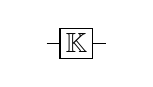
\begin{tikzpicture}[baseline={([yshift=-.5ex]current bounding box.center)}]
    \path (0,0) node (A) {}
    ++ (0.5,0) node[kernel] (K) {$\kernel{K}$}
    ++ (0.5,0) node (B) {};
    \draw (A) -- (K) -- (B);
\end{tikzpicture}\\
\mu&:= 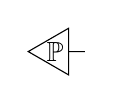
\begin{tikzpicture}[baseline={([yshift=-.5ex]current bounding box.center)}]
    \path (0,0) node[dist] (K) {$\kernel{P}$}
    ++ (0.5,0) node (B) {};
    \draw (K) -- (B);
\end{tikzpicture}
\end{align}

Given two Markov kernels $\kernel{L}:X\kto Y$ and $\kernel{M}:Y\kto Z$, the product $\kernel{L}\kernel{M}$ is represented by drawing them side by side and joining their wires:

\begin{align}
    \kernel{L}\kernel{M}:= 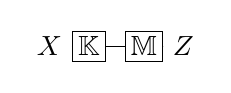
\begin{tikzpicture}[baseline={([yshift=-.5ex]current bounding box.center)}]
    \path (0,0) node (A) {$X$}
    ++ (0.5,0) node[kernel] (K) {$\kernel{K}$}
    ++ (0.7,0) node[kernel] (M) {$\kernel{M}$}
    ++ (0.5,0) node (B) {$Z$};
    \draw (A) -- (K) -- (M) -- (B);
\end{tikzpicture}
\end{align}

Given kernels $\kernel{K}:W\kto Y$ and $\kernel{L}:X\kto Z$, the tensor product $\kernel{K}\otimes\kernel{L}:W\times X\kto Y\times Z$ is graphically represented by drawing kernels in parallel:

\begin{align}
    \kernel{K}\otimes \kernel{L}&:=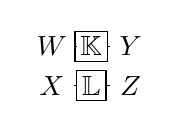
\begin{tikzpicture}[baseline={([yshift=-.5ex]current bounding box.center)}]
    \path (0,0) node (A) {$W$}
    ++ (0.5,0) node[kernel] (K) {$\kernel{K}$}
    ++ (0.5,0) node (B) {$Y$};
    \path (0,-0.5) node (C) {$X$}
    ++ (0.5,0) node[kernel] (L) {$\kernel{L}$}
    ++ (0.5,0) node (D) {$Z$};
    \draw (A) -- (K) -- (B);
    \draw (C) -- (L) -- (D);
\end{tikzpicture}
\end{align}

Given $\prob{K}:X\kto Y$ and $\prob{L}:Y\times X\kto Z$, the semidirect product is graphically represented by connecting $\kernel{K}$ and $\kernel{L}$ and keeping an extra copy

\begin{align}
    \prob{K}\cprod\prob{L}:&= \text{Copy}_X(\prob{K}\otimes \text{id}_X)(\text{Copy}_Y\otimes\text{id}_X )(\text{id}_Y \otimes \prob{L})\\
                            &= \tikzfig{copy_product}
\end{align}

A space $X$ is identified with the identity kernel $\mathrm{id}^X:X\to \Delta(\sigalg{X})$. A bare wire represents the identity kernel:

\begin{align}
\mathrm{Id}^X:=\begin{tikzpicture}
\path (0,0) node (X) {$X$}
++(2,0) node (Y) {$X$};
\draw (X) -- (Y);
\end{tikzpicture}
\end{align}

Product spaces $X\times Y$ are identified with tensor product of identity kernels $\mathrm{id}^X\otimes \mathrm{id}^Y$. These can be represented either by two parallel wires or by a single wire representing the identity on the product space $X\times Y$:
\begin{align}
X\times Y \cong \mathrm{Id}^X\otimes \mathrm{Id}^Y &:= 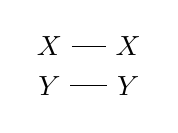
\begin{tikzpicture}
\path (0,0) node (E) {$X$}
++(1,0) node (F) {$X$}
(0,-0.5) node (F1) {$Y$}
+(1,0) node (G) {$Y$};
\draw (E) -- (F);
\draw (F1) -- (G);
\end{tikzpicture}\\
&= 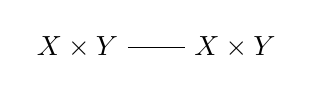
\begin{tikzpicture}
\path (0,0) node (X) {$X\times Y$}
++(2,0) node (Y) {$X\times Y$};
\draw (X) -- (Y);
\end{tikzpicture}
\end{align}

A kernel $\kernel{L}:X\to \Delta(\mathcal{Y}\otimes\mathcal{Z})$ can be written using either two parallel output wires or a single output wire, appropriately labeled:

\begin{align}
&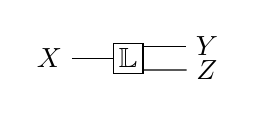
\begin{tikzpicture}
\path (0,0) node (E) {$X$}
++ (1,0) node[kernel] (L) {$\kernel{L}$}
++ (1,0.15) node (F) {$Y$}
+(0,-0.3) node (G) {$Z$};
\draw (E) -- (L);
\draw ($(L.east) + (0,0.15)$) -- (F);
\draw ($(L.east)+ (0,-0.15)$) -- (G);
\end{tikzpicture}\\
&\equiv\\
&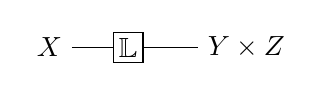
\begin{tikzpicture}
\path (0,0) node (E) {$X$}
++ (1,0) node[kernel] (L) {$\kernel{L}$}
++ (1.5,0) node (F) {$Y\times Z$};
\draw (E) -- (L) -- (F);
\end{tikzpicture}
\end{align}

We read diagrams from left to right (this is somewhat different to \citet{fritz_synthetic_2020,cho_disintegration_2019,fong_causal_2013} but in line with \citet{selinger_survey_2011}), and any diagram describes a set of nested products and tensor products of Markov kernels. There are a collection of special Markov kernels for which we can replace the generic ``box'' of a Markov kernel with a diagrammatic elements that are visually suggestive of what these kernels accomplish.

\subsection{Special maps}

\begin{definition}[Identity map]\label{def:ident_k}
The identity map $\text{Id}_X:X\kto X$ defined by $(\text{id}_X)(A|x)= \delta_x(A)$ for all $x\in X$, $A\in\sigalg{X}$, is represented by a bare line.
\begin{align}
    \mathrm{id}_X&:=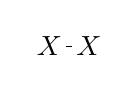
\begin{tikzpicture}[baseline={([yshift=-.5ex]current bounding box.center)}]
    \path (0,0) node (A) {$X$} ++ (0.5,0) node (B) {$X$};
    \draw (A) -- (B);
\end{tikzpicture}
\end{align}
\end{definition}

\begin{definition}[Erase map]\label{def:erase}
Given some 1-element set $\{*\}$, the erase map $\text{Del}_X:X\kto \{*\}$ is defined by $(\text{Del}_X)(*|x) = 1$ for all $x\in X$. It ``discards the input''. It looks like a lit fuse:
\begin{align}
    \text{Del}_X&:=\begin{tikzpicture}[baseline={([yshift=-.5ex]current bounding box.center)}]
    \path (0,0) ++ (1,0) node (B) {$X$};
    \draw[-{Rays[n=8]}] (A) -- (B);
\end{tikzpicture}
\end{align}
\end{definition}

\begin{definition}[Swap map]\label{def:swap}
The swap map $\text{Swap}_{X,Y}:X\times Y\kto Y\times X$ is defined by $(\text{Swap}_{X,Y})(A\times B|x,y)=\delta_x(B)\delta_y(A)$ for $(x,y)\in X\times Y$, $A\in \sigalg{X}$ and $B\in \sigalg{Y}$. It swaps two inputs and is represented by crossing wires:
\begin{align}
    \text{Swap}_{X,Y} &:=  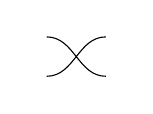
\begin{tikzpicture}[baseline={([yshift=-.5ex]current bounding box.center)}]
        \path (0,0) node (A) {} 
        + (0,-0.5) node (B) {}
        ++ (1,0) node (C) {}
        + (0,-0.5) node (D) {};
        \draw (A) to [out=0,in=180] (D) (B) to [out=0, in=180] (C);
    \end{tikzpicture}
\end{align}
\end{definition}

\begin{definition}[Copy map]\label{def:copy}
The copy map $\text{Copy}_X:X\kto X\times X$ is defined by $(\text{Copy}_X)(A\times B|x)=\delta_x(A)\delta_x(B)$ for all $x\in X$, $A,B\in \sigalg{X}$. It makes two identical copies of the input, and is drawn as a fork:
\begin{align}
    \text{Copy}_X&:=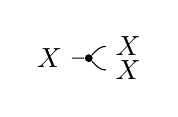
\begin{tikzpicture}[baseline={([yshift=-.5ex]current bounding box.center)}]
    \path (0,0) node (A) {$X$} 
    ++ (0.5,0) node[copymap] (copy0) {}
    ++ (0.5,0.15) node (B) {$X$}
    + (0,-0.3) node (C) {$X$};
    \draw (A) -- (copy0) to [out=45,in=180] (B) (copy0) to [out=-45, in=180] (C);
\end{tikzpicture}
\end{align}
\end{definition}

\begin{definition}[$n$-fold copy map]
The $n$-fold copy map $\text{Copy}^n_X:X\kto X^n$ is given by the recursive definition
\begin{align}
    \text{Copy}^1_X &= \text{Copy}_X\\
    \text{Copy}^n_X &= \tikzfig{n_fold_copy} &n>1
\end{align}
\end{definition}

\paragraph{Plates}\label{pgph:plates}

In a string diagram, a plate that is annotated $i\in A$ means the tensor product of the $|A|$ elements that appear inside the plate. A wire crossing from outside a plate boundary to the inside of a plate indicates an $|A|$-fold copy map, which we indicate by placing a dot on the plate boundary. For our purposes, we do not define anything that allows wires to cross from the inside of a plate to the outside; wires must terminate within the plate.

Thus, given $\kernel{K}_i:X\kto Y$ for $i\in A$,

\begin{align}
    \bigotimes_{i\in A} \kernel{K}_i &:= \tikzfig{plate_without_copymap}
    \text{Copy}^{|A|}_X(\bigotimes_{i\in A} \kernel{K}_i) &:= \tikzfig{plate_with_copymap}
\end{align}

\subsection{Commutative comonoid axioms}

Diagrams in Markov categories satisfy the commutative comonoid axioms.

\begin{align}
    \tikzfig{ccom_lhs} = \tikzfig{ccom_rhs}\label{eq:ccom_1}
\end{align}
\begin{align}
    \tikzfig{ccom2_lhs} = \tikzfig{ccom2_mhs} = \tikzfig{ccom2_rhs}\label{eq:ccom2_del}
\end{align}
\begin{align}
    \tikzfig{ccom3_lhs} = \tikzfig{ccom3_rhs} \label{eq:ccom3_swap}
\end{align}
as well as compatibility with the monoidal structure
\begin{align}
    \tikzfig{mstruct1_lhs} &= \tikzfig{mstruct1_rhs}\\
    \tikzfig{mstruct2_lhs} &= \tikzfig{mstruct2_rhs}
\end{align}
and the naturality of \emph{Del}, which means that
\begin{align}
    \tikzfig{naturality_lhs} &= \tikzfig{naturality_rhs}\label{eq:nat}
\end{align}


\subsection{Manipulating String Diagrams}\label{sssec:string_diagram_manipulation}

Planar deformations along with the applications of Equations \eqref{eq:ccom_1} through to Equation \eqref{eq:nat} are almost the only rules we have for transforming one string diagram into an equivalent one. One further rule is given by Theorem \ref{th:fong_det_kerns}.

\begin{theorem}[Copy map commutes for deterministic kernels \citep{fong_causal_2013}]\label{th:fong_det_kerns}
For $\kernel{K}:X\kto Y$
\begin{align}
	\tikzfig{deterministic_copymap_commute}
\end{align}
holds iff $\kernel{K}$ is deterministic.
\end{theorem}

\subsubsection{Examples}

String diagrams can always be converted into definitions involving integrals and tensor products. A number of shortcuts can help to make the translations efficiently.

For arbitrary $\kernel{K}:X\times Y\kto Z$, $\kernel{L}:W\kto Y$

\begin{align}
    \tikzfig{identity_tensor_L} &= (\text{id}_X\otimes \kernel{L})\kernel{K}\\
    [(\text{id}_X\otimes \kernel{L})\kernel{K}](A|x,w) &= \int_{Y}\int_X   \kernel{K}(A|x',y')\kernel{L}(\mathrm{d}y'|w)\delta_x(\mathrm{d}x')\\
                                           &= \int_Y  \kernel{K}(A|x,y') \kernel{L}(dy'|w)
\end{align}

That is, an identity map ``passes its input directly to the next kernel''. 

For arbitrary $\kernel{K}: X\times Y\times Y\kto Z$:

\begin{align}
 \tikzfig{identity_tensor_copy} &= (\text{id}_X\otimes \text{Copy}_Y)\kernel{K}\\
 [(\text{id}_X\otimes \text{Copy}_Y)\kernel{K}](A|x,y) &= \int_Y\int_Y \kernel{K}(A|x,y',y'') \delta_y(\mathrm{d}y')\delta_y(\mathrm{d}y'')\\
                                           &= \kernel{K}(A|x,y,y)
\end{align}

That is, the copy map ``passes along two copies of its input'' to the next kernel in the product. 

For arbitrary $\kernel{K}:X\times Y\kto Z$

\begin{align}
    \tikzfig{swap_example} &= \text{Swap}_{YX} \kernel{K}\\
    (\text{Swap}_{YX}\kernel{K})(A|y,x) &= \int_{X\times Y} \kernel{K}(A|x',y')\delta_y(\mathrm{d}y')\delta_x(\mathrm{d}x')\\
                                        &= \kernel{K}(A|x,y)
\end{align}

The swap map before a kernel switches the input arguments.

For arbitrary $\kernel{K}:X\kto Y\times Z$

\begin{align}
    \tikzfig{swap_example_2} &= \kernel{K}\text{Swap}_{YZ}\\
    (\kernel{K}\text{Swap}_{YZ})(A\times B|x) &= \int_{Y\times Z} \delta_{y}(B)\delta_{z}(A)\kernel{K}(\mathrm{d}y\times\mathrm{d}z|x)\\
    &= \int_{B\times A} \kernel{K}(\mathrm{d}y\times\mathrm{d}z|x)\\
    &= \kernel{K}(B\times A|x)
\end{align}

Given $\kernel{K}:X\kto Y$ and $\kernel{L}:Y\kto Z$:

\begin{align}
	(\kernel{K}\cprod \kernel{L})(\mathrm{id}_{Y}\otimes \mathrm{Del}_Z) &= \tikzfig{semidirect_K_L}\\
	 &= \tikzfig{semidirect_K_L_2} &\text{by Eq. \eqref{eq:nat}}\\
	 &= \tikzfig{semidirect_K_L_3} &\text{by Eq. \eqref{eq:ccom2_del}}
\end{align}

Thus the action of the $\text{Del}$ map is to marginalise over the deleted wire. With integrals, we can write

\begin{align}
	(\kernel{K}\cprod \kernel{L})(\mathrm{id}_{Y}\otimes \mathrm{Del}_Z)(A\times\{*\}|x) &= \int_{Y}\int_{\{*\}}\delta_y(A)\delta_{*}(\{*\})\kernel{L}(\mathrm{d}z|y)\kernel{K}(\mathrm{d}y|x)\\
	&= \int_A \kernel{K}(\mathrm{d}y|x)\\
	&= \kernel{K}(A|x)
\end{align}

\section{Symmetries of conditional probabilities}\label{app:io_contract_examples}

\subsection{Equality of equally sized contractions}\label{sec:equal_condits}

This is the proof of Theorem \ref{th:equal_of_condits}.

All swaps can be written as a product of transpositions, so proving that a property holds for all finite transpositions is enough to show it holds for all finite swaps. It's useful to define a notation for transpositions.

\begin{definition}[Finite transposition]
Given two equally sized sequences $A,B\in \mathbb{N}^n$ with $A=(a_i)_{i\in [n]}$, $B=(b_i)_{i\in [n]}$, ${A\rightarrow B}:\mathbb{N}\to \mathbb{N}$ is the permutation such that 
\begin{align}
    [A\rightarrow B](a_i) = b_i
\end{align}that sends the $i$th element of $A$ to the $i$th element of $B$ and vise versa. Note that $B\rightarrow A$ is the inverse of $A\rightarrow B$.
\end{definition}

Lemma \ref{lem:infinitely_extended_kernels} is used to extend conditional probabilities of finite sequences to infinite ones. 

\begin{lemma}[Infinitely extended kernels]\label{lem:infinitely_extended_kernels}
Given a collection of Markov kernels $\kernel{K}_i:W\times X^{\mathbb{N}}\kto Y^i$ for all $i\in \mathbb{N}$, if we have for every $j>i$
\begin{align}
    \kernel{K}_j(\text{id}_{Y^i}\otimes \text{Del}_{Y^{j-i}}) &= \kernel{K}_i\otimes \text{Del}_{X^{j-i}}\label{eqApp:marginalise_comb}
\end{align} 
then there is a unique Markov kernel $\kernel{K}:X^{\mathbb{N}}\kto Y^{\mathbb{N}}$ such that for all $i,j\in \mathbb{N}$,$j>i$
\begin{align}
    \kernel{K}(\text{id}_{Y^i}\otimes \text{Del}_{Y^{\mathbb{N}}})&= \kernel{K}_i\otimes \text{Del}_{X^{j-i}}
\end{align}
\end{lemma}

\begin{proof}
Take any $x\in X^{\mathbb{N}}$ and let $x_{|m}\in X^n$ be the first $n$ elements of $x$. By Equation \eqref{eqApp:marginalise_comb}, for any $A_i\in \sigalg{Y}$, $i\in [m]$
\begin{align}
    \kernel{K}_n(\bigtimes_{i\in [m]}A_i\times Y^{n-m}|x_{|n}) &= \kernel{K}_m(\bigtimes_{i\in [m]}A_i|x_{|m})
\end{align}

Furthermore, by the definition of the $\mathrm{Swap}$ map for any permutation $\rho:[n]\to[n]$
\begin{align}
    \kernel{K}_n\mathrm{Swap}_{\rho}(\bigtimes_{i\in [m]}A_{\rho(i)}\times Y^{n-m}|x_{|n}) &= \kernel{K}_n(\bigtimes_{i\in [m]}A_{i}\times Y^{n-m}|x_{|n})
\end{align}
thus by the Kolmogorov Extension Theorem \citep{cinlar_probability_2011}, for each $x\in X^{\mathbb{N}}$ there is a unique probability measure $\prob{Q}_x\in \Delta(Y^{\mathbb{N}}$ satisfying
\begin{align}
    \prob{Q}_x(\bigtimes_{i\in [n]}A_i\times Y^{\mathbb{N}}) &= \kernel{K}_n(\bigtimes_{i\in [n]}A_{\rho(i)}|x_{[n]})\label{eqApp:q_is_Markov}
\end{align}

Furthermore, for each $\{A_i\in\sigalg{Y}|i\in \mathbb{N}\}$, $n\in \mathbb{N}$ note that for $p>n$
\begin{align}
\prob{Q}_x(\bigtimes_{i\in[n]} A_i \times Y^{\mathbb{N}})&\geq \prob{Q}_x(\bigtimes_{i\in [p]} A_i\times Y^{\mathbb{N}})\\
&\geq \prob{Q}_x(\bigtimes_{i\in \mathbb{N}} A_i)
\end{align}
so by the Monotone convergence theorem, the sequence $\prob{Q}_x(\bigtimes_{i\in[n]} A_i)$ converges as $n\to \infty$ to $\prob{Q}_x(\bigtimes_{i\in\mathbb{N}} A_i)$. $x\mapsto \prob{Q}_x^{\RV{Z}_n}(\bigtimes_{i\in[n]} A_i)$ is measurable for all $n$, $\{A_i\in\sigalg{Y}|i\in \mathbb{N}\}$ by Equation \eqref{eqApp:q_is_Markov}, and so $x\mapsto Q_x$ is also measurable.

Thus $x\mapsto Q_x$ is the desired Markov kernel $\kernel{K}$.
\end{proof}

\begin{corollary}\label{cor:equal_subconditionals}
Given $(\prob{P}_C,\Omega,\sigalg{F})$, $\RV{W}:\Omega\to V$ and two pairs of sequences $(\RV{V},\RV{X}):=(\RV{V}_i,\RV{X}_i)_{i\in\mathbb{N}}$ and $(\RV{Y},\RV{Z}):=(\RV{Y}_i,\RV{Z}_i)_{i\in \mathbb{N}}$ with corresponding variables taking values in the same sets $V=Y$ and $X=Z$, if $(\prob{P}_C,\RV{V},\RV{X})$ and $(\prob{P}_C,\RV{Y},\RV{Z})$ are both local over $\RV{W}$ and
\begin{align}
    \prob{P}^{\RV{X}_{[n]}|\RV{W}\RV{V}_{[n]}} &= \prob{P}^{\RV{Z}_{[n]}|\RV{W}\RV{Y}_{[n]}}
\end{align}
for all $n\in\mathbb{N}$ then
\begin{align}
    \prob{P}^{\RV{X}|\RV{W}\RV{V}} &= \prob{P}^{\RV{Z}|\RV{W}\RV{Y}}
\end{align}
\end{corollary}

\begin{proof}
By assumption of locality
\begin{align}
    \prob{P}^{\RV{X}_{[n]}|\RV{W}\RV{V}_{[n]}}\otimes\mathrm{Del}_{W^\mathbb{N}} &= \prob{P}^{\RV{X}|\RV{W}\RV{V}}(\mathrm{id}_{X^n}\otimes \mathrm{Del}_{X^{\mathbb{N}}})\\
    \prob{P}^{\RV{Z}_{[n]}|\RV{W}\RV{Y}_{[n]}}\otimes\mathrm{Del}_{W^\mathbb{N}} &= \prob{P}^{\RV{Z}|\RV{W}\RV{Y}}(\mathrm{id}_{X^n}\otimes \mathrm{Del}_{X^{\mathbb{N}}})
\end{align}
hence for all $n,m>n$
\begin{align}
    \prob{P}^{\RV{X}_{[m]}|\RV{W}\RV{V}_{[m]}}(\mathrm{id}_{X^n}\otimes \mathrm{Del}_{X^{m-n}}) &= \prob{P}^{\RV{Z}_{[m]}|\RV{V}\RV{Y}_{[m]}}(\mathrm{id}_{X^n}\otimes \mathrm{Del}_{X^{m-n}})\\
    &= \prob{P}^{\RV{X}_{[n]}|\RV{W}\RV{V}_{[n]}}\otimes\mathrm{Del}_{W^{m-n}}
\end{align}
and, in particular, by lemma \ref{lem:infinitely_extended_kernels}, $\prob{P}^{\RV{X}|\RV{W}\RV{V}}$ and $\prob{P}^{\RV{Z}|\RV{W}\RV{Y}}$ are the limits of the same sequence.
\end{proof}

\begin{reptheorem}{th:equal_of_condits}
Given a sequential input-output model $(\prob{P}_C,\RV{D},\RV{Y})$ and some $\RV{W}$, $\prob{P}_\alpha^{\RV{Y}|\RV{WD}}$ is IO contractible over $\RV{W}$ if and only if for all subsequences $A,B\subset \mathbb{N}^{|A|}$ and for every $\alpha$
\begin{align}
    \prob{P}_\alpha^{\RV{Y}_A|\RV{WD}_{A,\mathbb{N}\setminus A}} &= \prob{P}_\alpha^{\RV{Y}_B|\RV{WD}_{B,\mathbb{N}\setminus B}}\\
    &= \prob{P}_\alpha^{\RV{Y}_A|\RV{WD}_A}\otimes \text{del}_{D^{|\mathbb{N}\setminus A|}}
\end{align}
\end{reptheorem}

\begin{proof}
Only if:
For $Z\in \mathbb{N}^{|A|}$, let $\text{del}_{Z^\complement}$ be the Markov kernel associated with the map that sends $\RV{Y}$ to $\RV{Y}_Z:=(\RV{Y}_i)_{i\in Z}$.

If $A$ is finite, then let $n:=|A|$ and by exchange commutativity
\begin{align}
        \prob{P}_\alpha^{\RV{Y}_A|\RV{WD_{A,\mathbb{N}\setminus A}}}&= \prob{P}_\alpha^{\RV{Y}_A|\RV{WD_{A\rightarrow [n]}}}\\
         &= \prob{P}_\alpha^{\RV{Y}|\RV{WD_{A\rightarrow [n]}}}\text{del}_{A^{\complement}}\\
        &=  \prob{P}_\alpha^{\RV{Y}_{[n]\rightarrow A}|\RV{WD}}\text{del}_{A^{\complement}}
\end{align}
Use the fact that $[n]\rightarrow A \circ B\rightarrow [n]= B\rightarrow A$ and apply exchange commutativity to get
\begin{align}
    \prob{P}_\alpha^{\RV{Y}_{[n]\rightarrow A}|\RV{WD}}\kernel{F}_{\Pi_{A}} &= \prob{P}_\alpha^{\RV{Y}_{B\rightarrow A}|\RV{WD}_{B\rightarrow [n]}}\text{del}_{A^{\complement}}\\
    &= \prob{P}_\alpha^{\RV{Y}|\RV{WD}_{B\rightarrow [n]}}\text{del}_{B^{\complement}}\\
    &= \prob{P}_\alpha^{\RV{Y}_B|\RV{WD_{B,\mathbb{N}\setminus B}}}
\end{align}

if $A$ is infinite, then we can take finite subsequences $A_m$ that are the first $m$ elements of $A$ and similarly for $B_m$. Then by previous reasoning
\begin{align}
            \prob{P}_\alpha^{\RV{Y}_{A_m}|\RV{WD_{A_m\rightarrow [m]}}} &= \prob{P}_\alpha^{\RV{Y}_{[m]}|\RV{WD}}\\
        &= \prob{P}_\alpha^{\RV{Y}_{B_m}|\RV{WD_{B_m\rightarrow [m]}}}
\end{align}
then by Corollary \ref{cor:equal_subconditionals}
\begin{align}
\prob{P}_\alpha^{\RV{Y}_A|\RV{WD_{A\rightarrow [n]}}}=\prob{P}_\alpha^{\RV{Y}_{B_m}|\RV{WD_{B_m\rightarrow [m]}}}
\end{align}

Finally, by locality
\begin{align}
    \prob{P}_\alpha^{\RV{Y}_A|\RV{WD_{A\rightarrow [n]}}} &= \prob{P}_\alpha^{\RV{Y}_A|\RV{WD}_A}\otimes \text{Del}_{D^{|\mathbb{N}\setminus A}}
\end{align}

If:
Taking $A=[n]$ for all $n$ establishes locality, and taking $A=(\rho(i))_{i\in \mathbb{N}}$ for arbitrary finite permutation $\rho$ establishes exchange commutativity.
\end{proof}

\subsection{Examples of symmetries}\label{app:examples_symmetries}

These are the examples referenced in Section \ref{sec:ccontracibility}. Example \ref{ex:no_implication} shows that neither locality nor exchange commutativity is implied by the other.

\begin{example}\label{ex:no_implication}
We prove the claim by way of presenting counterexamples.

First, a model that exhibits exchange commutativity but not locality. Suppose $D=Y=\{0,1\}$ and $\prob{P}_C^{\RV{Y}|\RV{D}}:D^{\mathbb{N}}\kto Y^{\mathbb{N}}$ is given by
\begin{align}
    \prob{P}_C^{\RV{Y}|\RV{D}}(\bigtimes_{i\in\mathbb{N}} A_i |(d_i)_{i\in\mathbb{N}}) &= \prod_{i\in \mathbb{N}} \delta_{\lim_{n\to\infty} \sum_{i\in\mathbb{N}} \frac{d_i}{n}}(A_i)
\end{align}
for some sequence $(d_i)_{i\in\mathbb{N}}$ such that this limit exists. Then for any finite permutation $\rho$
\begin{align}
    \prob{P}_C^{\RV{Y}_\rho|\RV{D}_\rho}(\bigtimes_{i\in\mathbb{N}} A_i |(d_i)_{i\in\mathbb{N}}) &= \prod_{i\in \mathbb{N}} \delta_{\lim_{n\to\infty} \sum_{i\in\mathbb{N}} \frac{d_{\rho^{-1}(i)}}{n}}(A_{\rho^{-1}(i)})\\
    &= \prob{P}_C^{\RV{Y}|\RV{D}}(\bigtimes_{i\in\mathbb{N}} A_i |(d_i)_{i\in\mathbb{N}})
\end{align}
so $(\prob{P}_C,\RV{D},\RV{Y})$ commutes with exchange, but
\begin{align}
    \prob{P}_C^{\RV{Y}_1|\RV{D}}(A_1 |0,1,1,1....) &= \delta_1(A_1)\\
    \prob{P}_C^{\RV{Y}_1|\RV{D}}(A_1 |0,0,0,0....) &= \delta_0(A_1)
\end{align}
so $(\prob{P}_C,\RV{D},\RV{Y})$ is not local.

Next, a model that satisfies locality but does not commute with exchange. Suppose again $D=Y=\{0,1\}$ and $\prob{P}_C^{\RV{Y}|\RV{D}}:D^{\mathbb{N}}\kto Y^{\mathbb{N}}$ is given by
\begin{align}
    \prob{P}_C^{\RV{Y}|\RV{D}}(\bigtimes_{i\in\mathbb{N}} A_i |(d_i)_{i\in\mathbb{N}}) &= \prod_{i\in \mathbb{N}} \delta_i(A_i)
\end{align}
then
\begin{align}
    \prob{P}_C^{\RV{Y}_\rho|\RV{D}_\rho}(\bigtimes_{i\in\mathbb{N}} A_i |(d_i)_{i\in\mathbb{N}}) &= \prod_{i\in \mathbb{N}} \delta_i(A_{\rho^{-1}(i)})\\
    &\neq \prod_{i\in \mathbb{N}} \delta_i(A_{i})\\
    =\prob{P}_C^{\RV{Y}|\RV{D}}(\bigtimes_{i\in\mathbb{N}} A_i |(d_i)_{i\in\mathbb{N}})
\end{align}
so $(\prob{P}_C,\RV{D},\RV{Y})$ does not commute with exchange but for all $n$
\begin{align}
    \prob{P}_C^{\RV{Y}_{[n]}|\RV{D}}(\bigtimes_{i\in[n]} A_i |(d_i)_{i\in\mathbb{N}}) &= \prod_{i\in [n]} \delta_i(A_{\rho^{-1}(i)})\\
    &= \prob{P}_C^{\RV{Y}_{[n]}|\RV{D}}(\bigtimes_{i\in[n]} A_i |(0)_{i\in\mathbb{N}})
\end{align}
so $(\prob{P}_C,\RV{D},\RV{Y})$ is local.
\end{example}

Although locality seems to an assumption that there is no interference between inputs and outputs of different indices, by itself it actually permits models with certain kinds of interference. This is shown in Example \ref{ex:interference_w_locality}.

\begin{example}\label{ex:interference_w_locality}
Consider an experiment where I first flip a coin and record the results of this flip as the outcome $\RV{Y}_1$ of ``step 1''. Subsequently, I can either copy the outcome from step 1 to the result for ``step 2'' (this is the input $\RV{D}_1=0$), or flip a second coin use this as the input for step 2 (this is the input $\RV{D}_1=1$). $\RV{D}_2$ is an arbitrary single-valued variable. Then for all $d_1, d_2$
\begin{align}
    \prob{P}^{\RV{Y}_1|\RV{D}}(y_1|d_1,d_2) &= 0.5\\
    \prob{P}^{\RV{Y}_2|\RV{D}}(y_2|d_1,d_2) &= 0.5
\end{align}
Thus the marginal distribution of both experiments in isolation is $\text{Bernoulli}(0.5)$ no matter what choices I make, but the input $\RV{D}_1$ affects the joint distribution of the results of both steps, which is not ruled out by locality.
\end{example}

\subsection[Representation]{Representation theorem preliminaries}\label{app:representation_proof}

This is the proof of Lemmas \ref{th:table_rep_kernel} and \ref{lem:ciid_yd} and Theorem \ref{th:any_infinite_sequence} from Section \ref{sec:rep_theorem_background}. In addition, Lemmas \ref{lem:ciid_yd} and \ref{lem:hw_interchange} are presented and proved, which will be later used in the proof of Theorem \ref{th:ciid_rep_kernel}.

The following definitions are reproduced for the reader's convenience. Note that these proofs use the string diagram notation explained in Appendix \ref{ssec:mken_diagrams}.

\begin{repdefinition}{def:count_of_inputs}
Given a sequential input-output model $(\prob{P}_{\cdot},\RV{D},\RV{Y})$ on $(\Omega,\sigalg{F})$ with countable $D$, $\#_{j}^k$ is the variable
\begin{align}
    \#_{j}^k := \sum_{i=1}^{k-1} \llbracket \RV{D}_i = j \rrbracket
\end{align}
In particular, $\#_{j}^k$ is equal to the number of times $\RV{D}_i=j$ over all $i<k$.
\end{repdefinition}

\begin{repdefinition}{def:tab_cd}
Given a sequential input-output model $(\prob{P}_{\cdot},\RV{D},\RV{Y})$ on $(\Omega,\sigalg{F})$, define the tabulated conditional distribution $\RV{Y}^D:\Omega\to Y^{\mathbb{N}\times D}$ by
\begin{align}
    \RV{Y}^D_{ij} = \sum_{k=1}^{\infty} \llbracket \#_j^k = i-1\rrbracket \llbracket \RV{D}_k = j \rrbracket \RV{Y}_k
\end{align}
That is, the $(i,j)$-th coordinate of $\RV{Y}^D(\omega)$ is equal to the coordinate $\RV{Y}_k(\omega)$ for which the corresponding $\RV{D}_k(\omega)$ is the $i$th instance of the value $j$ in the sequence $(\RV{D}_1(\omega),\RV{D}_2(\omega),...)$, or 0 if there are fewer than $i$ instances of $j$ in this sequence.
\end{repdefinition}

\begin{replemma}{th:table_rep_kernel}
Suppose a sequential input-output model $(\prob{P}_C,\RV{D},\RV{Y})$ is given with $D$ countable and $\RV{D}$ infinitely supported. Then for some $\RV{W}$, $\alpha$, $\prob{P}_\alpha^{\RV{Y}|\RV{WD}}$ is IO contractible if and only if
\begin{align}
    \prob{P}_\alpha^{\RV{Y}|\RV{WD}} &= \tikzfig{lookup_representation_kernel}\label{eqApp:lup_rep_kernel}\\
    &\iff\\
    \prob{P}_\alpha^{\RV{Y}|\RV{WD}}(\bigtimes_{i\in \mathbb{N}}A_i|w,(d_i)_{i\in \mathbb{N}}) &= \prob{P}_\alpha^{(\RV{Y}^D_{i d_i})_{i\in\mathbb{N}}|\RV{W}}(\bigtimes_{i\in \mathbb{N}}A_i|w)&\forall A_i\in \sigalg{Y}^{D}, w\in W, d_i\in D
\end{align}
Where $\prob{F}_{\text{lu}}$ is the Markov kernel associated with the lookup map
\begin{align}
    \text{lu}:X^\mathbb{N}\times Y^{\mathbb{N}\times D}&\to Y\\
    ((x_i)_\mathbb{N},(y_{ij})_{i,j\in \mathbb{N}\times D})&\mapsto (y_{i d_i})_{i\in \mathbb{N}}
\end{align}
and for any finite permutation within rows $\eta:\mathbb{N}\times D\to \mathbb{N}\times D$
\begin{align}
    \prob{P}_\alpha^{(\RV{Y}^D_{ij})_{\mathbb{N}\times D}|\RV{W}}&= \prob{P}_\alpha^{(\RV{Y}^D_{\eta(i,j)})_{\mathbb{N}\times D}|\RV{W}}\label{eqApp:col_exch}
\end{align}
\end{replemma}

\begin{proof}
Only if:
We define a random invertible function $\RV{R}:\Omega\times \mathbb{N}\to \mathbb{N}\times {D}$ that reorders the indicies so that, for $i\in \mathbb{N},j\in D$, $\RV{D}_{\RV{R}^{-1}(i,j)}=j$ almost surely. We then use IO contractibility to show that $\prob{P}_\alpha^{\RV{Y}|\RV{D}}(\cdot|d)$ is equal to the distribution of the elements of $\RV{Y}^D$ selected according to $d\in D^{\mathbb{N}}$.

Note that at most one of $\llbracket \#_j^k = i-1\rrbracket\llbracket \RV{D}_k=j\rrbracket$ and $\llbracket \#_j^l = i-1\rrbracket\llbracket \RV{D}_l=j\rrbracket$ can be greater than 0 for $k\neq l$ and, by assumption, $\sum_{j\in D}\sum_{k\in \mathbb{N}} \llbracket \#_j^k = i-1\rrbracket\llbracket \RV{D}_k=j\rrbracket=1$ almost surely (that is, for any $i,j$ there is some $k$ such that $\RV{D}_k$ is the $i$th occurrence of $j$). Define $\RV{R}_k:\Omega\to \mathbb{N}\times D$ by $\omega \mapsto \argmax_{i\in\mathbb{N},j\in D} \llbracket \#_j^k = i-1\rrbracket\llbracket \RV{D}_k=j\rrbracket(\omega)$ (i.e. $\RV{R}_k$ returns the $(i,j)$ pair where $j$ is the value of $\RV{D}_k$ and $i$ is the count of $j$ occurrences up to $\RV{D}_k$). Let $\RV{R}:\mathbb{N}\to \mathbb{N}\times D$ by $k\mapsto \RV{R}_k$. $\RV{R}$ is almost surely bijective and 
\begin{align}
    \RV{Y}^D&:= (\RV{Y}^D_{ij})_{i\in \mathbb{N},j\in D}\\
    &= (\RV{Y}_{\RV{R}^{-1}(i,j)})_{i\in \mathbb{N},j\in D}\\
    &=: \RV{Y}_{\RV{R}^{-1}}
\end{align}

By construction, $\RV{D}_{\RV{R}^{-1}(i,j)}=j$ almost surely; that is, $\RV{D}_{\RV{R}^{-1}}$ is a single-valued variable. In particular, it is almost surely equal to $e:=(e_{ij})_{i\in\mathbb{N},j\in D}$ such that $e_{ij}=j$ for all $i$. Hence
\begin{align}
    \prob{P}_\alpha^{\RV{Y}^D|\RV{W}\RV{D}_{\RV{R}^{-1}}}(A|w,d)&= \prob{P}_\alpha^{\RV{Y}_{\RV{R}^{-1}}|\RV{W}\RV{D}_{\RV{R}^{-1}}}(A|w,d)\\
    &\overset{\prob{P}_{\cdot}}{\cong} \prob{P}_\alpha^{\RV{Y}_{\RV{R}^{-1}}|\RV{W}\RV{D}_{\RV{R}^{-1}}}(A|w,e)\label{eqApp:yd_is_indep}\\
    &= \prob{P}_\alpha^{\RV{Y}^D}(A|w)\label{eqApp:yd_dist}
\end{align}
for any $d\in D^{\mathbb{N}}$.

Now,
\begin{align}
    \prob{P}^{\RV{Y}_{\RV{R}^{-1}}|\RV{W}\RV{D}_{\RV{R}^{-1}}}_\alpha(A|w,d) &= \int_R \prob{P}_\alpha^{\RV{Y}_\rho|\RV{W}\RV{D}_{\rho}}(A|d)\prob{P}_\alpha^{\RV{R}^{-1}|\RV{W}\RV{D}_{\RV{R}^{-1}}}(\mathrm{d}\rho|w,d)\label{eqApp:need_ccont}\\
\end{align}
For each $\rho$, define $\rho^n:\mathbb{N}\to \mathbb{N}$ as the finite permutation that agrees with $\rho$ on the first $n$ indices and is the identity otherwise. By IO contractibility, for $n\in \mathbb{N}$
\begin{align}
    \prob{P}^{\RV{Y}_{\rho^n([n])}|\RV{W}\RV{D}_{\rho^n([n])}} &= \prob{P}^{\RV{Y}_{\rho([n])}|\RV{W}\RV{D}_{\rho([n])}}\\
    &= \prob{P}^{\RV{Y}_{[n]}|\RV{W}\RV{D}_{[n]}}
\end{align}
By Corollary \ref{cor:equal_subconditionals}, it must therefore be the case that
\begin{align}
    \prob{P}^{\RV{Y}|\RV{W}\RV{D}} = \prob{P}^{\RV{Y}_{\rho}|\RV{W}\RV{D}_{\rho}}
\end{align}
Then from Equation \eqref{eqApp:need_ccont}
\begin{align}
    \prob{P}^{\RV{Y}_{\RV{R}^{-1}}|\RV{W}\RV{D}_{\RV{R}^{-1}}}_\alpha(A|w,d) &\overset{\prob{P}_{\cdot}}{\cong} \int_R \prob{P}_\alpha^{\RV{Y}_\rho|\RV{W}\RV{D}_{\rho}}(A|d)\prob{P}_\alpha^{\RV{R}^{-1}|\RV{W}\RV{D}_{\RV{R}^{-1}}}(\mathrm{d}\rho|w,d)\\
    &\overset{\prob{P}_{\cdot}}{\cong} \int_R \prob{P}_{\cdot}^{\RV{Y}|\RV{WD}}(A|w,d)\prob{P}_\alpha^{\RV{R}^{-1}|\RV{W}\RV{D}_{\RV{R}^{-1}}}(\mathrm{d}\rho|w,d)\\
    &\overset{\prob{P}_{\cdot}}{\cong} \prob{P}_{\cdot}^{\RV{Y}|\RV{WD}}(A|w,d)\label{eqApp:rotated_conditional}
\end{align}
 for all $i,j\in \mathbb{N}$. Then by Equation \eqref{eqApp:yd_dist} and Equation \eqref{eqApp:rotated_conditional}
\begin{align}
    \prob{P}_\alpha^{\RV{Y}^D|\RV{W}}(A|w) &= \prob{P}_\alpha^{\RV{Y}|\RV{WD}}(A|w,e)\label{eqApp:rel_bet_y_yd}
\end{align}

Take some $d\in D^{\mathbb{N}}$. From Equation \eqref{eqApp:rel_bet_y_yd} and IO contractibility of $\prob{P}_{\cdot}^{\RV{Y}|\RV{WD}}(A|e)$,
\begin{align}
    (\prob{P}_\alpha^{\RV{Y}^D|\RV{W}}\otimes \mathrm{id}_D)\kernel{F}_{lu}(A|w,d) &= \prob{P}_\alpha^{(\RV{Y}^D_{i d_i})_{i\in \mathbb{N}}|\RV{W}}(A|d)\\
    &=\prob{P}_\alpha^{(\RV{Y}_{i d_i})_{i\in \mathbb{N}}|\RV{WD}}(A|w,e)\\
    &= \prob{P}_\alpha^{(\RV{Y}_{i d_i})_{i\in \mathbb{N}}|\RV{W}(\RV{D}_{i d_i})_{\mathbb{N}})}(A|w,(e_{i d_i})_{i\in \mathbb{N}})\\
    &= \prob{P}_\alpha^{\RV{Y}|\RV{WD}}(A|w,(e_{i d_i})_{i\in \mathbb{N}})\\
    &= \prob{P}_\alpha^{\RV{Y}|\RV{WD}}(A|w,(d_i)_{i\in\mathbb{N}})
\end{align}

It remains to be shown that $\RV{Y}^D$ is invariant to finite permutations within rows. Consider some finite permutation within columns $\eta:\mathbb{N}\times D\to \mathbb{N}\times D$, note that $e_{\eta(i,j)}=j$ and hence $(e_{\eta(i,j)})_{i\in\mathbb{N},j\in D}=e$. Thus
\begin{align}
    \prob{P}_\alpha^{(\RV{Y}^D_{\eta_(i,j)})_{\mathbb{N}\times D}|\RV{W}}(A|w) &= \prob{P}_\alpha^{(\RV{Y}^D)_{\mathbb{N}\times D}|\RV{W}}\text{Swap}_{\eta}(A|w)\\
    &= \prob{P}_\alpha^{\RV{Y}|\RV{WD}}\text{Swap}_{\eta}(A|w,e)&\text{from Eq. }\eqref{eqApp:rel_bet_y_yd}\\
    &= \prob{P}_\alpha^{\RV{Y}_\eta|\RV{WD}}(A|w,e)\\
    &= \prob{P}_\alpha^{\RV{Y}|\RV{WD}_{\eta^{-1}}}(A|w,e)&\text{by exchange commutativity}\\
    &= \prob{P}_\alpha^{\RV{Y}|\RV{WD}}(A|w,(e_{\eta^{-1}(i,j)})_{i\in \mathbb{N},j\in D})\\
    &= \prob{P}_\alpha^{\RV{Y}|\RV{WD}}(A|w,e)\\
    &= \prob{P}_\alpha^{(\RV{Y}^D_{ij})_{\mathbb{N}\times D}|\RV{W}}(A|w)&\text{from Eq. }\eqref{eqApp:rel_bet_y_yd}
\end{align}

If:
We construct a conditional probability according to Definition \ref{def:tab_cd} and verify that it satisfies IO contractibility.

Suppose 
\begin{align}
    \prob{P}_\alpha^{\RV{Y}|\RV{WD}} &= \tikzfig{lookup_representation_kernel}
\end{align}
where $\prob{P}_\alpha^{\RV{Y}^D|\RV{W}}$ satisfies Equation \eqref{eqApp:col_exch}.

Consider any two $d,d'\in D^{\mathbb{N}}$ such that for some $S,T\subset\mathbb{N}$ with $|S|=|T|=n$, $d_S=d'_T$. Let $S\leftrightarrow T$ be the transposition that swaps the $i$th element of $S$ with the $i$th element of $T$ for all $i$.
\begin{align}
    \prob{P}_\alpha^{\RV{Y}_S|\RV{WD}}(\bigtimes_{i\in [n]} A_i|w,d) &= \prob{P}_\alpha^{(\RV{Y}^D_{i d_i})_{i\in S}|\RV{W}} (\bigtimes_{i\in [n]} A_i|w)\\
    &= \prob{P}_\alpha^{(\RV{Y}^D_{S\leftrightarrow T(i) d_i})_{i\in S}|\RV{W}} (\bigtimes_{i\in [n]} A_i|w)\\
    &= \prob{P}_\alpha^{(\RV{Y}^D_{i d_{S\leftrightarrow T(i)}})_{i\in T}|\RV{W}} (\bigtimes_{i\in [n]} A_i|w)\\
    &= \prob{P}_\alpha^{(\RV{Y}^D_{i d'_{i}})_{i\in T}|\RV{W}} (\bigtimes_{i\in [n]} A_i|w)\\
    &=  \prob{P}_\alpha^{\RV{Y}_T|\RV{WD}}(\bigtimes_{i\in [n]} A_i|w,d')
\end{align}
and, in particular, taking $T=[n]$
\begin{align}
    &= \prob{P}_\alpha^{\RV{Y}_{[n]}|\RV{WD}} (\bigtimes_{i\in [n]} A_i|w,d')
\end{align}
but $d'$ is an arbitrary sequence such that the $T$ elements match the $S$ elements of $d$, so this holds for any other $d''$ whose $T$ elements also match the $S$ elements of $d$. That is
\begin{align}
    \prob{P}_\alpha^{\RV{Y}_S|\RV{WD}}(\bigtimes_{i\in [n]} A_i|w,d)&= (\prob{P}_\alpha^{\RV{Y}_{[n]}|\RV{WD}_{[n]}}\otimes \mathrm{Del}_{D^{\mathbb{N}}}) (\bigtimes_{i\in [n]} A_i|w,d')
\end{align}
so $\kernel{K}$ is IO contractible by Theorem \ref{th:equal_of_condits}.
\end{proof}

As a consequence of Lemma \ref{th:table_rep_kernel} along with De Finetti's representation theorem, we can say that given $(\prob{P}_{\cdot},\RV{D},\RV{Y})$ IO contractible, conditioning on $\RV{H}$ renders the columns of $\RV{Y}^D$ independent and identically distributed.

\begin{lemma}\label{lem:ciid_yd}
Suppose a sequential input-output model $(\prob{P}_{\cdot},\RV{D},\RV{Y})$ is given with $D$ countable, $\RV{D}$ infinitely supported over some $\RV{W}$ and $(\prob{P}_\cdot,\RV{D},\RV{Y})$ IO contractible over the same $\RV{W}$. Then, letting $\RV{H}$ be the directing random conditional of $(\prob{P}_{\cdot},\RV{D},\RV{Y})$ (Definition \ref{def:dir_rand_cond}) and $\RV{Y}^D_{iD}:=(\RV{Y}^D_{ij})_{j\in D}$, we have for all $i\in\mathbb{N}$, $\RV{Y}^D_{iD}\CI^e_{\prob{P}_{\cdot}} (\RV{Y}^D_{\mathbb{N}\setminus\{i\}D},\RV{W},\text{id}_C) | \RV{H}$ and
\begin{align}
    \prob{P}_C^{\RV{Y}^D_{iD}|\RV{H}}(A|\nu) \overset{\prob{P}_\alpha}{\cong} \nu(A)
\end{align}
\end{lemma}

\begin{proof}
Fix $w\in W$ and consider $\prob{P}_{\alpha,w}^{\RV{Y}^D}:= \prob{P}_{\alpha}^{\RV{Y}^D|\RV{W}}(\cdot|w)$. From Lemma \ref{th:table_rep_kernel}, we have the exchangeability of the sequence $(\RV{Y}^D_{1D},\RV{Y}^D_{2D},...)$ with respect to $(\prob{P}_{\alpha,w},\Omega,\sigalg{F})$ as a special case of the invariance of $\prob{P}_\alpha^{(\RV{Y}^D_{ij})_{\mathbb{N}\times D}|\RV{W}}$ to permutations of rows. By the column exchangeability of $\prob{P}_{\alpha,w}^{\RV{Y}^D}$, from \citet[Prop. 1.4]{kallenberg_basic_2005} (where $\RV{H}$ is precisely what Kallenberg calls the directing random measure)
\begin{align}
    \prob{P}_{\alpha,w}^{\RV{Y}^D|\RV{H}} &= \tikzfig{de_finetti_conditional}
\end{align}
Because the right hand side does not depend on $w$, we can say
\begin{align}
    \prob{P}_{\alpha}^{\RV{Y}^D|\RV{HW}} &= \tikzfig{de_finetti_conditional_erase}
\end{align}
and because it also does not depend on $\alpha$ we have $\RV{Y}^D\CI^e_{\prob{P}_{\cdot}} (\RV{W},\text{id}_C) | \RV{H}$. Further application of \citet[Prop. 1.4]{kallenberg_basic_2005} yields $\RV{Y}^D_{iD}\CI^e_{\prob{P}_{\cdot}} (\RV{Y}^D_{\mathbb{N}\setminus\{i\}D},\RV{W}) | (\RV{H},\text{id}_C)$ and
\begin{align}
    \prob{P}_\alpha^{\RV{Y}^D_{iD}|\RV{H}}(A|\nu) \overset{\prob{P}_\alpha}{\cong} \nu(A)
\end{align}
Again, the right hand side does not depend on $\alpha$, which yields $\RV{Y}^D_{iD}\CI^e_{\prob{P}_{\cdot}} (\RV{Y}^D_{\mathbb{N}\setminus\{i\}D},\RV{W},\text{id}_C) | \RV{H}$.
\end{proof}


\begin{reptheorem}{th:any_infinite_sequence}
Suppose a sequential input-output model $(\prob{P}_\cdot,\RV{D},\RV{Y})$ is given with $D$ countable,  $\RV{D}$ infinitely supported and for some $\RV{W}$, $\prob{P}_\alpha^{\RV{Y}|\RV{WD}}$ is IO contractible for all $\alpha$. Consider an infinite set $A\subset \mathbb{N}$, and let $\RV{D}_A:=(\RV{D}_i)_{i\in A}$ and $\RV{Y}_A:=(\RV{Y}_i)_{i\in A}$. Then $\RV{H}_A$, the directing random conditional of $(\prob{P}_{\cdot},\RV{D}_A,\RV{Y}_A)$ is almost surely equal to $\RV{H}$, the directing random conditional of $(\prob{P}_{\cdot},\RV{D},\RV{Y})$.
\end{reptheorem}

\begin{proof}
The strategy we will pursue is to show that an arbitrary subsequence of $(\RV{D}_i,\RV{Y}_i)$ pairs induces a random contraction of the rows of $\RV{Y}^D$. Then we show that the contracted version of $\RV{Y}^D$ has the same distribution as the original, and consequently the normalised partial sums converge to the same limit.

Define $\RV{Y}^{D,A}$ as the tabulated conditional of $(\RV{D}_A,\RV{Y}_A)$, i.e. let $\#^{A,k}_j$ be the count restricted to $A$:
\begin{align}
    \#^{A,k}_j := \sum_{i\in A}^{k-1} \llbracket \RV{D}_i = j \rrbracket
\end{align}
then
\begin{align}
    \RV{Y}^{D,A}_{ij} &:= \sum_{k\in A} \llbracket\#^{A,k}_j=i-1\rrbracket\llbracket \RV{D}_k=j\rrbracket \RV{Y}_k\\
        &= \sum_{k\in A} \llbracket\#^{A,k}_j=i-1\rrbracket\llbracket \RV{D}_k=j\rrbracket \RV{Y}^D_{\RV{R}_k j}
\end{align}
That is, defining $\RV{Q}:\mathbb{N}\to \mathbb{N}$ by $i\mapsto \sum_{k\in A} \llbracket\#^{A,k}_j=i-1\rrbracket\llbracket \RV{D}_k=j\rrbracket \RV{R}_k$ then
\begin{align}
    \RV{Y}^{D,A}_{ij} &= \RV{Y}^D_{\RV{Q}(i) j}\label{eqApp:random_contraction}
\end{align}
where $\RV{Q}(i)\in \mathbb{N}$ by the assumption that each value of $D$ occurs infinitely often in $A$ (otherwise $\RV{Q}(i)$ might be 0).

Equation \eqref{eqApp:random_contraction} is what is meant by ``the subsequence $(\RV{D}_A,\RV{Y}_A)$ induces a random contraction over the rows of $\RV{Y}^D$''. We will now show that $\RV{Y}^{D,A}$ has the same distribution as $\RV{Y}^D$.

Let $\text{con}_{q}:Y^{\mathbb{N}\times D}\kto Y^{\mathbb{N}\times D}$ be the Markov kernel associated with the function that sends $(\RV{Y}^D_{ij})_{i\in \mathbb{N},j\in D}$ to $(\RV{Y}^D_{q(i)j})_{i\in \mathbb{N},j\in D}$. Then for any $B\in \sigalg{Y}^{\mathbb{N}\times D}$, $w,q$:
\begin{align}
    \prob{P}_\alpha^{\RV{Y}^{D,A}|\RV{WQ}}(B|w,q) &= \prob{P}_\alpha^{\RV{Y}^D|\RV{W}}\text{con}_q(B|w)\\
    &= \prob{P}_\alpha^{\RV{Y}|\RV{WD}}\text{con}_q(B|w,e)&\text{by Eq.} \eqref{eqApp:rel_bet_y_yd}\\
    &= \prob{P}_\alpha^{\RV{Y}|\RV{WD}}(B|w,e)&\text{by Theorem }\ref{th:equal_of_condits}\\
    &= \prob{P}_\alpha^{\RV{Y}^D|\RV{W}}(B|w)&\text{by Eq.} \eqref{eqApp:rel_bet_y_yd}\label{eqApp:equal_of_tabs}
\end{align}

Finally, take $\RV{H}_A$ the directing random measure of $\RV{Y}^{D,A}$. We conclude from the equality Eq. \eqref{eqApp:equal_of_tabs} and from the fact that there is a one-to-one map from directing random measures to exchangeable distributions that $\RV{H}_A\overset{\prob{P}_\alpha}{\cong} \RV{H}$.
\end{proof}

The following is a technical lemma that will be used in Theorem \ref{th:ciid_rep_kernel}.

\begin{lemma}\label{lem:hw_interchange}
Suppose a sequential input-output model $(\prob{P}_{\cdot},\RV{D},\RV{Y})$ is given with $D$ countable, $\RV{D}$ infinitely supported over $\RV{W}$, for some $\RV{W}$, $\prob{P}_\alpha^{\RV{Y}|\RV{WD}}$ is IO contractible for all $\alpha$ and for all $\alpha$
\begin{align}
    \prob{P}_\alpha^{\RV{Y}|\RV{WD}} &= \tikzfig{lookup_representation_kernel}\label{eq:lup_rep_kernel_2}
\end{align}
then $\RV{Y}\CI^e_{\prob{P}_{\cdot}} \RV{W} | (\RV{H},\RV{D},\text{id}_C)$ and for all $\alpha$
\begin{align}
    \prob{P}_{\alpha}^{\RV{Y}|\RV{HD}} &= \tikzfig{lookup_representation_kernel_h}
\end{align}
\end{lemma}

\begin{proof}
We show that the function that maps the variables $\RV{Y}$ and $\RV{D}$ to $\RV{H}$ also maps $\RV{Y}^D$ and the constant $e\in D^{\mathbb{N}}$ to $\RV{H}'$ with $\RV{H}'\overset{\prob{P}_{\cdot}}{\cong} \RV{H}$, and the result follows from disintegration along with a conditional independence given by Lemma \ref{th:table_rep_kernel}.

$\RV{Y}^D$ is a function of $\RV{Y}$ and $\RV{D}$ (see Definition \ref{def:tab_cd}) and $\RV{H}$ is a function of $\RV{Y}^D$. Say $f:Y\times D\to H$ is such that $\RV{H}=f(\RV{Y},\RV{D})$ (see Definition \ref{def:dir_rand_meas}). Because $\RV{H}=f(\RV{Y},\RV{D})$, we have $\RV{H}\CI^e_{\prob{P}_C} (\RV{W},\text{id}_C)|(\RV{Y},\RV{D})$. Thus
\begin{align}
    \prob{P}_\alpha^{\RV{YH}|\RV{WD}} &= \tikzfig{lookup_representation_kernel_joint}\label{eqApp:luprep_joint}
\end{align}
For a sequence $d\in D^{\mathbb{N}}$ where each $j\in D$ occurs infinitely often, take $[d=j]_i$ to be the $i$th coordinate of $d$ equal to $j\in D$ and $\#_{[d=j]_i}$ to be the position in $d$ of $[d=j]_i$. Concretely, $f$ is given by
\begin{align}
    f(y,d) &= \bigtimes_{j\in D} A_j \mapsto \lim_{n\to \infty} \frac{1}{n}\sum_{i=1}^n \prod_{j\in D} \mathds{1}_{A_j}(y_{\#_{[d=j]_i}})\\
    &=: f_d(y)
\end{align}
where the limit exists. Note that for $y^D\in Y^{D\times\mathbb{N}}$ we have
\begin{align}
    f_d\circ \mathrm{lu}(y^D,d) &= \bigtimes_{j\in D} A_j \mapsto \lim_{n\to \infty} \frac{1}{n}\sum_{i=1}^n \prod_{j\in D} \mathds{1}_{A_j}(y^D_{\#_{[d=j]_i} j})
\end{align}
Let $g:=(y^D,d)\mapsto f_d\circ \mathrm{lu}(y^D,d)$ for some $d\in D^{\mathbb{N}}$ where each $j\in D$ occurs infinitely often.

We aim to show that $g(\RV{Y}^D,d)\overset{\prob{P}_\alpha}{\cong} g(\RV{Y}^D,d')$ for all $d,d'\in D^{\mathbb{N}}$ such that each $j\in D$ occurs infinitely often.

Consider, for arbitrary $A\in \sigalg{Y}^D$
\begin{align}
    \prob{P}_\alpha (g(\RV{Y}^D,d)(A)\yields g(\RV{Y}^D,d')(A)) &= \int_H \prob{P}_\alpha^{\mathrm{Id}_{\Omega}|\RV{H}}(g(\RV{Y}^D,d)(A)\yields g(\RV{Y}^D,d')(A)|\nu)\prob{P}_\alpha^{\RV{H}}(\mathrm{d}\nu)
\end{align}

Note that
\begin{align}
     \prob{P}_\alpha^{\mathrm{Id}_{\Omega}|\RV{H}}(g(\RV{Y}^D,d)(A)\yields \nu(A)|\nu) &= \prob{P}_\alpha^{\RV{Y}^D|\RV{H}}(\lim_{n\to\infty}\frac{1}{n}\sum_{i=1}^n \prod_{j\in D} \mathds{1}_{A_j}(y^D_{\#_{[d=j]_i},j})\yields \nu(A)| \nu)\prob{P}_\alpha^{\RV{H}}(\mathrm{d}\nu)
\end{align}
by independent permutability of the rows of $\RV{Y}^D$ (Lemma \ref{th:table_rep_kernel}), for each row we can send $\#_{[d=j]_i}$ to $i$ and obtain
\begin{align}
    \prob{P}_\alpha^{\RV{Y}^D|\RV{H}}(\lim_{n\to\infty}\frac{1}{n}\sum_{i=1}^n \prod_{j\in D} \mathds{1}_{A_j}(y^D_{\#_{[d=j]_i},j})\yields \nu(A)| \nu)\prob{P}_\alpha^{\RV{H}}(\mathrm{d}\nu) &= \prob{P}_\alpha^{\RV{Y}^D|\RV{H}} (\lim_{n\to\infty}\frac{1}{n}\sum_{i=1}^n \prod_{j\in D} \mathds{1}_{A_j}(y^D_{i,j})\yields \nu(A)| \nu)\\
    &= \prob{P}_\alpha^{\RV{Y}^D_{iD}|\RV{H}} (\lim_{n\to\infty}\frac{1}{n}\sum_{i=1}^n \mathds{1}_{A}(y^D_{i,D})\yields \nu(A)| \nu)
\end{align}
but by Lemma \ref{lem:ciid_yd}, the sequence $(\RV{Y}^D_{iD})_{i\in \mathbb{N}}$ are mutually independent conditional on $\RV{H}$ and for all $\alpha$, $\prob{P}_\alpha^{\RV{Y}_{iD}|\RV{H}}(A|\nu)\overset{\prob{P}_C}{\cong}\nu(A)$. Thus, by the law of large numbers
\begin{align}
    \prob{P}_\alpha^{\RV{Y}^D|\RV{H}} (\lim_{n\to\infty}\frac{1}{n}\sum_{i=1}^n \mathds{1}_{\prod_{j\in D} A_j}(y^D_{i,D})\yields \nu(A)| \nu)&= 1
\end{align}
which implies
\begin{align}
     &\phantom{=}\int_H \prob{P}_\alpha^{\mathrm{Id}_{\Omega}|\RV{H}}(g(\RV{Y}^D,d)(A)\yields g(\RV{Y}^D,d')(A)|\nu)\prob{P}_\alpha^{\RV{H}}(\mathrm{d}\nu) \\
     &= \int_H \prob{P}_\alpha^{\mathrm{Id}_{\Omega}|\RV{H}}(g(\RV{Y}^D,d)(A)\yields \nu(A) \cap  g(\RV{Y}^D,d')(A)\yields \nu(A)|\nu)\prob{P}_\alpha^{\RV{H}}(\mathrm{d}\nu)\\
    &= 1
\end{align}

Because this holds for all $A$,
\begin{align}
    g(\RV{Y}^D,d)&\overset{\prob{P}_\alpha}{\cong} g(\RV{Y}^D,d') & \text{as this holds for all }A
\end{align}
And, as a consequence, defining
\begin{align}
    i:(y^d,d,d')\mapsto (\mathrm{lu}(\RV{Y}^D,d),g(\RV{Y}^D,d'))
\end{align}
we have
\begin{align}
    i(y^d,d,d) &\overset{\prob{P}_\alpha}{\cong} i(y^d,d,d')
\end{align}
which in turn implies the almost sure equality of the associated Markov kernels:
\begin{align}
     \tikzfig{hw_interchange_2} &= \tikzfig{hw_interchange_3}
\end{align}
but we also have, by the definitions of $f$ and $g$
\begin{align}
    \tikzfig{hw_interchange_1} &=  \tikzfig{hw_interchange_2}
\end{align}
we can therefore write $\prob{P}_\alpha^{\RV{YH}|\RV{WD}}$ as
\begin{align}
    &\phantom{=} \tikzfig{lookup_representation_kernel_joint}\\
    &= \tikzfig{lookup_representation_kernel_joint_half}\\
    &=: \tikzfig{lookup_representation_kernel_joint_2}
\end{align}
because $\RV{H}$ is a deterministic function of $\RV{Y}^D$, this implies
\begin{align}
    \prob{P}_\alpha^{\RV{YH}|\RV{WD}} &= \tikzfig{lookup_representation_kernel_joint_2_subbed}\label{eq:sub_in_lookup}
\end{align}

Noting that $\kernel{F}_h\otimes\mathrm{Del}_W = \prob{P}_\alpha^{\RV{H}|\RV{Y}^D\RV{W}}$
\begin{align}
    \prob{P}_\alpha^{\RV{Y}^D\RV{H}|\RV{W}} &= \tikzfig{p_yd_on_w} \\
    &= \tikzfig{yd_h_on_w_invert} \label{eq:yd_on_h}
\end{align}
and so by substituting Equation \eqref{eq:yd_on_h} into \eqref{eq:sub_in_lookup}
\begin{align}
    \prob{P}_\alpha^{\RV{YH}|\RV{WD}} &= \tikzfig{lookup_representation_kernel_joint_3}
\end{align}
From Lemma \ref{th:table_rep_kernel} we also have $\RV{Y}^D\CI^e_{\prob{P}_C} (\RV{W},\text{id}_C)|\RV{H}$ , so
\begin{align}
    \prob{P}_\alpha^{\RV{YH}|\RV{WD}} &= \tikzfig{lookup_representation_kernel_joint_4}\label{eqApp:disintegrate_twice}
\end{align}
and so by higher order conditionals $\RV{Y}\CI^e_{\prob{P}_C} \RV{W} | (\RV{H},\RV{D},\text{id}_C)$ and
\begin{align}
    \prob{P}_{\alpha}^{\RV{Y}|\RV{HD}} &= \tikzfig{lookup_representation_kernel_h}
\end{align}
Because the right hand side does not depend on $\alpha$, we finally have $\RV{Y}\CI^e_{\prob{P}_C} (\RV{W},\text{id}_C) | (\RV{H},\RV{D})$ and the result
\begin{align}
    \prob{P}_{C}^{\RV{Y}|\RV{HD}} &= \tikzfig{lookup_representation_kernel_h}
\end{align}
Furthermore, by marginalising the right hand side of Equation \ref{eqApp:disintegrate_twice} we have
\begin{align}
    \prob{P}_\alpha^{\RV{H}|\RV{WD}} &= \tikzfig{lookup_representation_kernel_joint_4_marged}
\end{align}
Hence $\RV{H} \CI^e_{\prob{P}_C} \RV{D} | (\RV{W},\text{id}_C)$.
\end{proof}

\subsection{Representation theorem}\label{sec:io_contract_models}

This is the proof of the main result from Section \ref{sec:evaluating_decisions}, Theorem \ref{th:ciid_rep_kernel}. 

\begin{reptheorem}{th:ciid_rep_kernel}
Suppose a sequential input-output model $(\prob{P}_C,\RV{D},\RV{Y})$ with sample space $(\Omega,\sigalg{F})$ is given with $D$ countable and $\RV{D}$ infinitely supported. Then the following are equivalent:
\begin{enumerate}
    \item There is some $\RV{W}$ such that $\prob{P}_\alpha^{\RV{Y}|\RV{WD}}$ is IO contractible for all $\alpha$
    \item For all $i$, $\RV{Y}_i\CI^e_{\prob{P}_C} (\RV{Y}_{\neq i},\RV{D}_{\neq i},\text{id}_C)|(\RV{H},\RV{D}_i)$ and for all $i,j$ $$\prob{P}_C^{\RV{Y}_i|\RV{H}\RV{D}_i}=\prob{P}_C^{\RV{Y}_j|\RV{H}\RV{D}_j}$$
    \item There is some $\kernel{L}:H\times X\kto Y$ such that $$\prob{P}_C^{\RV{Y}|\RV{HD}}= \tikzfig{do_model_representation_conditional}$$
\end{enumerate}
\end{reptheorem}

\begin{proof}
As a preliminary, we will show
\begin{align}
    \kernel{F}_{\mathrm{lu}} &= \tikzfig{lookup_rep_intermediate_kernel}\label{eqApp:ev_alternate_rep}
\end{align}
where  $\mathrm{lus}:D\times Y^D\to Y$ is the single-shot lookup function
\begin{align}
    ((y_i)_{i\in D},d)\mapsto y_d
\end{align}

Recall that $\mathrm{lu}$ is the function
\begin{align}
    ((d_i)_\mathbb{N},(y_{ij})_{i,j\in \mathbb{N}\times D})&\mapsto (y_{i d_i})_{i\in \mathbb{N}}
\end{align}
By definition, for any $\{A_i\in\sigalg{Y}|i\in \mathbb{N}\}$
\begin{align}
    \kernel{F}_{\mathrm{lu}}(\bigtimes_{i\in \mathbb{N}}A_i|(d_i)_\mathbb{N},(y_{ij})_{i\in \mathbb{N}\times D}) &= \delta_{(y_{i d_i})_{i\in \mathbb{N}}}(\bigtimes_{i\in \mathbb{N}}A_i)\\
        &= \prod_{i\in \mathbb{N}} \delta_{y_{i d_i}} (A_i)\\
        &= \prod_{i\in \mathbb{N}} \kernel{F}_{\text{evs}} (A_i|d_i,(y_{ij})_{j\in D})\\
        &= \left(\bigotimes_{i\in\mathbb{N}} \kernel{F}_{\mathrm{evs}} \right)(\bigtimes_{i\in \mathbb{N}}A_i|(d_i)_\mathbb{N},(y_{ij})_{i,j\in \mathbb{N}\times D})
\end{align}
which is what we wanted to show.

(1)$\implies$(3):
From Lemma \ref{th:table_rep_kernel}, we have some $\RV{Y}^D$ such that
\begin{align}
    \prob{P}_{\alpha}^{\RV{Y}|\RV{WD}} &= \tikzfig{lookup_representation_kernel}
\end{align}
and by Lemma \ref{lem:ciid_yd}
\begin{align}
    \prob{P}_{C}^{\RV{Y}^D|\RV{H}} &= \tikzfig{de_finetti_conditional_w_upd}\label{eqApp:df_rep_mu}\\
\end{align}

By Lemma \ref{th:table_rep_kernel}, for each $w\in W$
\begin{align}
    \prob{P}_{\alpha}^{\RV{Y}|\RV{WD}} &= \tikzfig{lookup_representation_kernel}
\end{align}
and so by Lemma \ref{lem:hw_interchange}
\begin{align}
    \prob{P}_{C}^{\RV{Y}|\RV{HD}} &= \tikzfig{lookup_representation_kernel_h}\label{eqApp:lu_rep_h}
\end{align}

We can substitute Equations \eqref{eqApp:df_rep_mu} and \eqref{eqApp:ev_alternate_rep} into \eqref{eqApp:lu_rep_h} for
\begin{align}
    \prob{P}_{C}^{\RV{Y}|\RV{HD}} &= \tikzfig{do_model_representation_conditional}
\end{align}

(3)$\implies$ (2):
If
\begin{align}
    \prob{P}_{C}^{\RV{Y}|\RV{HD}} &= \tikzfig{do_model_representation_conditional}
\end{align}
then by the definition of higher order conditionals, for any $i\in \mathbb{N}$ and any $\alpha\in C$
\begin{align}
    \prob{P}_C^{\RV{Y}_i|\RV{HD}_i\RV{Y}_{\neq i}\RV{D}_{\neq i}} &\overset{\prob{P}_C}{\cong} \kernel{L}\otimes \text{Del}_{Y^{\mathbb{N}}\times X^{\mathbb{N}}}
\end{align}
hence $\RV{Y}_i\CI^e_{\prob{P}_C} (\RV{Y}_{\neq i},\RV{D}_{\neq i},\text{id}_C)|(\RV{H},\RV{D}_i)$

(2)$\implies$ (1):
Take $\RV{W}:=\RV{H}$. Because we assume $\RV{Y}_i\CI^e_{\prob{P}_C} (\RV{Y}_{[1,i)},\RV{D}_{[1,i),\text{id}_C})|(\RV{H},\RV{D}_i)$ we can take $\kernel{L}:= \prob{P}_\alpha^{\RV{Y}_i|\RV{H}\RV{X}_i}$ for arbitrary $i$ (by assumption, they are all the same) and
\begin{align}
    \prob{P}_C^{\RV{Y}_i|\RV{HD}_i\RV{Y}_{[1,i)}\RV{D}_{[1,i)}} &\overset{\prob{P}_C}{\cong} \kernel{L}\otimes \text{Del}_{Y^{i-1}\times X^{i-1}}
\end{align}
by taking the semidirect product of the conditionals
\begin{align}
    \prob{P}_{C}^{\RV{Y}|\RV{HD}} &= \tikzfig{do_model_representation_conditional}\\
    &= \tikzfig{do_model_representation_conditional_permuted}
\end{align}
hence $(\prob{P}_C,\RV{D},\RV{Y})$ is exchange commutative over $\RV{H}$. Furthermore, take $A\subset \mathbb{N}$. Then
\begin{align}
    &\tikzfig{do_model_representation_conditional_deleted}\\
    =& \tikzfig{do_model_representation_conditional_deleted1}
\end{align}
so $(\prob{P}_C,\RV{D},\RV{Y})$ is also local over $\RV{H}$.
\end{proof}

\subsection{Data-independent models}\label{sec:data_independent_proofs}

Theorem \ref{th:ciid_rep_kernel} says that a data independent sequential input-output model $(\prob{P}_{\cdot},\RV{D},\RV{Y})$ features conditionally independent and identical response functions $\prob{P}_\alpha^{\RV{Y}_i|\RV{HD}_i}$ for all $\alpha$ if and only if there is some $\RV{W}$ such that $\prob{P}_\alpha^{\RV{Y}|\RV{WD}}$ is IO contractible over $\RV{W}$ for all $\alpha$. The variable $\RV{W}$ is something of a nuisance; rather than thinking only about whether IO contractibility holds, we must consider whether there's \emph{any} variable that licenses the assumption of IO contractibility.

A simple special case to consider is when $\RV{W}$ is single valued -- that is, when $\prob{P}_\alpha^{\RV{Y}|\RV{D}}$ is IO contractible. As Theorem \ref{th:data_ind_CC} shows, this corresponds to the CIIR sequence models where the inputs $\RV{D}$ are unconditionally data-independent and independent of the hypothesis $\RV{H}$. We can also consider the case where $(\prob{P}_{\cdot}, \RV{D},\RV{Y})$ is only exchange commutative over $*$. This corresponds to models where the inputs $\RV{D}$ are data-independent and the hypothesis $\RV{H}$ depends on a symmetric function of the inputs $\RV{D}$ (under some side conditions).


\begin{theorem}[Data-independent IO contractibility]\label{th:data_ind_CC}
Suppose a sequential input-output model $(\prob{P}_{\cdot},\RV{D},\RV{Y})$ with sample space $(\Omega,\sigalg{F})$ is given with $D$ countable and, letting $E\subset D^{\mathbb{N}}$ be the set of all sequences for which each $j\in D$ occurs infinitely often, $\prob{P}_\alpha^{\RV{D}}(E)=1$ for all $\alpha$. Then the following are equivalent:
\begin{enumerate}
    \item $\prob{P}_\alpha^{\RV{Y}|\RV{D}}$ is IO contractible for all $\alpha$
    \item For all $i$, $\RV{Y}_i\CI^e_{\prob{P}_{\cdot}} (\RV{Y}_{\neq i},\RV{D}_{\neq i},\text{id}_C)|(\RV{H},\RV{D}_i)$, for all $i,j,\alpha$ $$\prob{P}_\alpha^{\RV{Y}_i|\RV{H}\RV{D}_i}=\prob{P}_\alpha^{\RV{Y}_j|\RV{H}\RV{D}_j}$$, $\RV{H}\CI^e_{\prob{P}_{\cdot}} \RV{D}|\text{id}_C$ and for all $i$ $\RV{D}_i\CI^e_{\prob{P}_{\cdot}} \RV{D}_{(i,\infty]}) | (\RV{D}_{[1,i)},\text{id}_C)$
    \item There is some $\kernel{L}:H\times X\kto Y$ such that for all $\alpha$, $$\prob{P}_\alpha^{\RV{YH}|\RV{D}}= \tikzfig{do_model_representation_with_h}$$
\end{enumerate}
\end{theorem}

\begin{proof}
See Appendix \ref{sec:data_independent_proofs}.
\end{proof}

While $\prob{P}_{\cdot}^{\RV{Y}|\RV{D}}$ exchange commutative is not necessarily IO contractible, exchange commutativity of this conditional implies IO contractibility over the directing random conditional $\RV{H}$, and thus is sufficient for conditionally independent and identical responses.

\begin{theorem}\label{lem:exch_prod_ciid}
If $\prob{P}_{\alpha}^{\RV{Y}|\RV{D}}$ is exchange commutative, and for each $\alpha$ $\prob{P}_\alpha^{\RV{D}}$ is absolutely continuous with respect to some exchangeable distribution $\prob{Q}_\alpha^{\RV{D}}$ in $\Delta(D^{\mathbb{N}})$ with directing random measure $\RV{F}$ and $\RV{D}$ infinitely supported over $\RV{F}$ with respect to $\prob{Q}_\alpha$ , then $\prob{P}_\alpha^{\RV{Y}|\RV{HD}}$ is IO contractible, where $\RV{H}$ is the directing random conditional for $\prob{P}_\alpha^{\RV{Y}|\RV{D}}$.
\end{theorem}

\begin{proof}
We show that there is an exchangeable distribution for which the relevant conditional automatically satisfies IO contractibility and is almost surely equal to $\prob{P}_\alpha^{\RV{Y}|\RV{GD}}$ for some $\RV{G}$.
\end{proof}

\begin{lemma}[Exchangeably dominated conditionals]\label{lem:dom_cond}
Given $(\prob{P}_C,\Omega,\sigalg{F})$ and variables $\RV{D},\RV{Y}$, if for any $\alpha$ there is some $\prob{Q}_\alpha$ such that $\prob{Q}_\alpha^{\RV{DY}}$ is exchangeable with directing random measure $\RV{G}$, $\RV{D}$ is infinitely supported over $\RV{G}$ with respect to $\prob{Q}_\alpha$ and for any $i$, $\prob{Q}_\alpha^{\RV{Y}_i|\RV{D}\RV{Y}_{\{i\}^{\complement}}}\overset{\prob{P}}{\cong} \prob{P}_\alpha^{\RV{Y}_i|\RV{D}\RV{Y}_{\{i\}^{\complement}}}$ then $\prob{P}_\alpha^{\RV{Y}|\RV{HD}}$ is IO contractible (where $\RV{H}$ is the directing random conditional for $\prob{P}_\alpha^{\RV{Y}|\RV{D}}$).
\end{lemma}

\begin{proof}
By \citet[Prop. 1.4]{kallenberg_basic_2005}, there is a $\RV{G}$ such that $(\RV{D}_i,\RV{Y}_i)\CI^e_{\prob{Q}_C} (\RV{D}_{\{i\}^{\complement}}\RV{Y}_{\{i\}^{\complement}})|(\RV{G},\text{id}_C)$ and for all $i,j$
\begin{align}
    \prob{Q}_\alpha^{\RV{Y}_i\RV{D}_i|\RV{G}} &= \prob{Q}_\alpha^{\RV{Y}_j\RV{D}_j|\RV{G}}\label{eqApp:joint_given_g}
\end{align}

There is some function $f:D^{\mathbb{N}}\times Y^{\mathbb{N}}$ such that $\RV{G}=f(\RV{D},\RV{Y})$, i.e.
\begin{align}
    \prob{Q}_\alpha^{\RV{Y_iG}|\RV{D}\RV{Y}_{\{i\}^{\complement}}} &= \tikzfig{qyg_eq_pyg}\\
                                     &\overset{P}{\cong} \prob{P}_\alpha^{\RV{Y_iG}|\RV{D}\RV{Y}_{\{i\}^{\complement}}}\\
    \implies \prob{Q}_\alpha^{\RV{Y_i}|\RV{G}\RV{D}\RV{Y}_{\{i\}^{\complement}}}&\overset{P}{\cong} \prob{P}_\alpha^{\RV{Y}_i|\RV{G}\RV{D}\RV{Y}_{\{i\}^{\complement}}}\label{eqApp:cond_on_g}
\end{align}

It follows from weak union that
\begin{align}
    \RV{Y}_i\CI^e_{\prob{Q}_C} (\RV{D}_{\{i\}^{\complement}}\RV{Y}_{\{i\}^{\complement}}) | (\RV{D}_i,\RV{G},\text{id}_C)\\
    \iff \prob{P}_\alpha^{\RV{Y}_i|\RV{D}_i\RV{G}\RV{Y}_{\{i\}^{\complement}}\RV{D}_{\{i\}^{\complement}}}(A|d_i,g,d,y) &\overset{P}{\cong} \prob{P}_\alpha^{\RV{Y}_i|\RV{D}_i\RV{G}}(A|d_i,g) & \forall A,d_i,g,d,y,\alpha\label{eqApp:swap_q_for_p}\\
    \implies \RV{Y}_i\CI^e_{\prob{P}_C} (\RV{D}_{\{i\}^{\complement}}\RV{Y}_{\{i\}^{\complement}}) | (\RV{D}_i,\RV{G},\text{id}_C)
\end{align}
where Eq. \eqref{eqApp:swap_q_for_p} follows from Eq. \eqref{eqApp:cond_on_g}.

Finally, from Eq. \eqref{eqApp:joint_given_g} and Eq. \eqref{eqApp:swap_q_for_p}
\begin{align}
    \prob{P}_\alpha^{\RV{Y}_i|\RV{D}_i\RV{G}} &\overset{\prob{P}}{\cong} \prob{P}_\alpha^{\RV{Y}_j\RV{D}_j|\RV{G}}
\end{align}
Thus $(\prob{P}_C,\RV{D},\RV{Y})$ features independent and identical responses conditioned on $\RV{G}$, and by Lemma \ref{lem:ci_drc} it also has independent and identical responses conditioned on $\RV{H}$. Finally, the infinite support of $\RV{D}$ over $\RV{G}$ with respect to $\RV{Q}_\alpha$ implies $\RV{D}$ is also infinitely supported over $\RV{G}$ with respect to $\prob{P}_\alpha$, so by Theorem \ref{th:ciid_rep_kernel} $\prob{P}_\alpha^{\RV{Y}|\RV{HD}}$ is IO contractible.
\end{proof}

\begin{reptheorem}{th:infinite_condition_swaps}
A data-independent sequential input-output model $(\prob{P}_C,\RV{D},\RV{Y})$ features conditionally independent and identical response functions $\prob{P}_\alpha^{\RV{Y}_i|\RV{D}_i\RV{G}}$ with $\RV{D}$ infinitely supported over $\RV{G}$ only if for any sets $A,B\subset \mathbb{N}$ such that $\RV{D}_A$ and $\RV{D}_B$ are also infinitely supported over $\RV{G}$ and any $i,j\in \mathbb{N}$ such that $i\not\in A$, $j\not\in B$, $$\prob{P}_\alpha^{\RV{Y}_i|\RV{D}_i\RV{Y}_A,\RV{D}_A}=\prob{P}_\alpha^{\RV{Y}_j|\RV{D}_j|RV{Y}_B\RV{D}_B}$$.  If in addition each $\prob{P}_\alpha^{\RV{YD}}$ is dominated by some $\prob{Q}_\alpha$ such that $\prob{Q}_\alpha^{\RV{Y}\RV{D}}$ is exchangeable, then the reverse implication also holds.
\end{reptheorem}

\begin{proof}
Only if: By Theorem \ref{th:ciid_rep_kernel} and Lemma \ref{lem:ci_drc}, $\prob{P}_\alpha^{\RV{Y}|\RV{HD}}$ is IO contractible. By Theorem \ref{th:any_infinite_sequence}, $\RV{H}$ is almost surely a function of both $(\RV{D}_A,\RV{Y}_A)$ and $(\RV{D}_B,\RV{Y}_B)$ and, furthermore, $\RV{Y}_i\CI_{\prob{P}_C}^e (\RV{D}_A,\RV{Y}_A)|(\RV{D}_i,\RV{H},\text{id}_C)$, $\RV{Y}_j\CI_{\prob{P}_C}^e (\RV{D}_B,\RV{Y}_B)|(\RV{D}_j,\RV{H},\text{id}_C)$. Hence there is some $f:D^{\mathbb{N}}\times Y^{\mathbb{N}}\to H$ such that for all $E\in \sigalg{Y}, d_i\in D, d\in D^{\mathbb{N}}, y\in Y^{\mathbb{N}}$
\begin{align}
    \prob{P}_\alpha^{\RV{Y}_i|\RV{D}_i\RV{Y}_A,\RV{D}_A}(E|d_i,y,d) &= \prob{P}_\alpha^{\RV{Y}_i|\RV{D}_i\RV{H}}(E|d_i,f(y,d))\\
     &= \prob{P}_\alpha^{\RV{Y}_j|\RV{D}_j\RV{H}}(E|d_i,f(y,d))\label{eqApp:eq_cond}\\
     &= \prob{P}_\alpha^{\RV{Y}_j|\RV{D}_j\RV{Y}_B,\RV{D}_B}(E|d_i,y,d)
\end{align}
Where Eq. \eqref{eqApp:eq_cond} follows from Theorem \ref{th:equal_of_condits}.

If:
By construction
\begin{align}
    \prob{Q}_\alpha^{\RV{Y}_i\RV{D}_i\RV{Y}_{\{i^{\complement}\}}\RV{D}_{\{i^{\complement}\}}}:=\prob{Q}_\alpha^{\RV{D}_i\RV{Y}_{\{i^{\complement}\}}\RV{D}_{\{i^{\complement}\}}}\odot \prob{P}_\alpha^{\RV{Y}_i|\RV{D}_i\RV{Y}_{\{i^{\complement}\}},\RV{D}_{\{i^{\complement}\}}}
\end{align}
is exchangeable, and by domination $\prob{Q}_\alpha^{\RV{Y}_i|\RV{D}_i\RV{Y}_{\{i^{\complement}\}},\RV{D}_{\{i^{\complement}\}}}\overset{\prob{P}}{\cong}\prob{Q}_\alpha^{\RV{Y}_i|\RV{D}_i\RV{Y}_{\{i^{\complement}\}},\RV{D}_{\{i^{\complement}\}}}$. The result follows from Lemma \ref{lem:dom_cond}.
\end{proof}

\begin{theorem}[Copy map commutes for deterministic kernels \citep{fong_causal_2013}]\label{th:fong_det_kerns}
For $\kernel{K}:X\kto Y$
\begin{align}
    \tikzfig{deterministic_copymap_commute}
\end{align}
holds iff $\kernel{K}$ is deterministic.
\end{theorem}

\begin{theorem}\label{lem:exch_prod_ciid}
Given $(\prob{P}_cdot,\RV{Y},\RV{D})$, if $\prob{P}_\alpha^{\RV{Y}|\RV{D}}$ is exchange commutative for each $\alpha$, and for each $\alpha$ $\prob{P}_\alpha^{\RV{D}}$ is absolutely continuous with respect to some exchangeable distribution $\prob{Q}_\alpha^{\RV{D}}$ in $\Delta(D^{\mathbb{N}})$ with directing random measure $\RV{F}$ and $\RV{D}$ is infinitely supported over $\RV{F}$ with respect to $\prob{Q}_\alpha$, then $(\prob{P}_cdot,\RV{Y},\RV{D})$.
\end{theorem}

\begin{proof}
For each $\alpha$, extend $\prob{Q}_\alpha^{\RV{D}}$ to a distribution on $(\RV{D},\RV{Y})$ by asserting that $\prob{P}_\alpha^{\RV{Y}|\RV{D}}\overset{\prob{Q}_\alpha}{\cong} \prob{Q}_\alpha^{\RV{Y}|\RV{D}}$. Because $\prob{Q}_\alpha^{\RV{D}}$ dominates $\prob{P}_\alpha^{\RV{D}}$, we have in fact $\prob{Q}_\alpha^{\RV{Y}|\RV{D}}\overset{\prob{P}}{\cong}\prob{P}_\alpha^{\RV{Y}|\RV{D}}$

We will show $\prob{Q}_\alpha^{\RV{DY}}$ is unchanged by finite permutations of $(\RV{D}_i,\RV{Y}_i)$ pairs. For some finite permutation $\rho:\mathbb{N}\to\mathbb{N}$:
\begin{align}
    \prob{Q}_\alpha^{\RV{D}_\rho\RV{Y}_\rho} &= \prob{Q}_\alpha^{\RV{D}_\rho\RV{Y}_\rho} (\text{Swap}_{\rho,D^{\mathbb{N}}}\otimes \text{Swap}_{\rho,Y^{\mathbb{N}}})\\
    &= \prob{Q}_\alpha^{\RV{D}}\odot \prob{Q}_\alpha^{\RV{Y}|\RV{D}}(\text{Swap}_{\rho,D^{\mathbb{N}}}\otimes \text{Swap}_{\rho,Y^{\mathbb{N}}})\\
    &= \tikzfig{exch_dom_swap1}\\
    &= \tikzfig{exch_dom_swap2}\\
    &= \tikzfig{exch_dom_swap3}\label{eqApp:exch_comep}\\
    &= \tikzfig{exch_dom_swap4}\label{eqApp:det_comep}\\
    &= \tikzfig{exch_dom_swap5}\label{eqApp:exchep}\\
    &= \prob{Q}_\alpha^{\RV{D}\RV{Y}}
\end{align}
Where line \eqref{eqApp:exch_comep} follows from exchange commutativity, \eqref{eqApp:det_comep} follows from Theorem \ref{th:fong_det_kerns} and the fact that the swap map is deterministic and line \eqref{eqApp:exchep} comes from the exchangeability of $\prob{Q}_\alpha^{\RV{D}}$.

Because $\prob{P}_\alpha^{\RV{D}}$ is dominated by $\prob{Q}_\alpha^{\RV{D}}$ by assumption, we have $\prob{P}_\alpha^{\RV{Y}|\RV{D}} \overset{\prob{P}}{\cong} \prob{Q}_\alpha^{\RV{Y}|\RV{D}}$, which implies $\prob{Q}_\alpha^{\RV{Y}_i|\RV{D}\RV{Y}_{\{i\}^{\complement}}}\overset{\prob{P}}{\cong} \prob{Q}_\alpha^{\RV{Y}_i|\RV{D}\RV{Y}_{\{i\}^{\complement}}}$ and from Lemma \ref{lem:dom_cond} we therefore have $\prob{P}_\alpha^{\RV{Y}|\RV{HD}}$ IO contractible over $\RV{H}$, and from Theorem \ref{th:ciid_rep_kernel} we have $\RV{Y}\CI^e_{\prob{P}_C} \text{id}_C | (\RV{D},\RV{H})$ and so $\prob{P}_\alpha^{\RV{Y}|\RV{HD}}$ IO contractible over $\RV{H}$ also.
\end{proof}

\section{Precedented options}\label{sec:proof_precedent}

This is the proof of Theorem \ref{th:latent_to_observable} in Section \ref{sec:precedent}.

\begin{repdefinition}{def:diverse_precedent}
Given a see-do model $(\prob{P}_\cdot,(\RV{E}_i,\RV{X}_i,\RV{Y}_i,\RV{Z}_i)_{i\in\mathbb{N}\cup\{c\}})$ with $E,X,Y$ and $Z$ all discrete sets, suppose among the observations $i\in \mathbb{N}$ the pairs $(\RV{Z}_i,(\RV{E}_i,\RV{X}_i,\RV{Y}_i))$ share conditionally independent and identical responses and, for all observations and consequences $i\in \mathbb{N}\cup\{c\}$, pairs $(\RV{E}_i,(\RV{X}_i,\RV{Y}_i))$ also share conditionally independent and identical responses.

Take $\RV{G}$ to be the directing random conditional of $(\prob{P}_\cdot,\RV{Z}_{\mathbb{N}},(\RV{E}_i,\RV{X}_i,\RV{Y}_i)_{i\in \mathbb{N}})$. 

We say that the options $C$ have \emph{diverse precedent} with respect to $(\prob{P}_\cdot,(\RV{E}_i,\RV{X}_i,\RV{Y}_i,\RV{Z}_i)_{i\in\mathbb{N}\cup\{c\}})$ if for all $\alpha$, $\prob{P}_\alpha$-almost all $z,z'\in Z$, $e\in E$, $g^E_{z}\in \Delta(E)$, $g^{XY}_{EZ}\in \Delta(X\times Y)^{E\times Z}$, $\prob{P}_\alpha$ satisfies the condition:
\begin{align}
    \prob{P}_{\alpha}^{\RV{G}^E_{z'}|\RV{G}^{XY}_{EZ}\RV{G}^E_{z}}(\cdot|g^{XY}_{EZ},g^E_{z}) \ll U_{\Delta(E)}\label{eq:lebesgue_dom}
\end{align}
Where $U_{\Delta(E)}$ is the uniform measure on the $|E-1|$ simplex of discrete probability distributions with $|E|$ outcomes.
\end{repdefinition}

\begin{reptheorem}{th:latent_to_observable}
Given a see-do model $(\prob{P}_\cdot,(\RV{E}_i,\RV{X}_i,\RV{Y}_i,\RV{Z}_i)_{i\in\mathbb{N}\cup\{c\}})$ with $E,X,Y$ and $Z$ all discrete sets, suppose among the observations $i\in \mathbb{N}$ the pairs $(\RV{Z}_i,(\RV{E}_i,\RV{X}_i,\RV{Y}_i))$ share conditionally independent and identical responses and, for all observations and consequences $i\in \mathbb{N}\cup\{c\}$, pairs $(\RV{E}_i,(\RV{X}_i,\RV{Y}_i))$ also share conditionally independent and identical responses. Take $\RV{G}$ to be the directing random conditional of $(\prob{P}_\cdot,\RV{Z}_{\mathbb{N}},(\RV{E}_i,\RV{X}_i,\RV{Y}_i)_{i\in \mathbb{N}})$.

Let $I\subset \Delta(Y)^{XZ}$ be the event $\RV{G}^Y_{Xz}=\RV{G}^Y_{Xz'}$ for all $z,z'\in Z$; i.e. the event that $\RV{Y}_i$ is independent of $\RV{Z}_i$ conditional on $\RV{X}_i$ and $\RV{G}$. Define $\prob{Q}_\alpha\in \Delta(\Omega)$ to be the probability measure such that, for all $A\in \sigalg{F}$
\begin{align}
\prob{Q}_\alpha(A) := \prob{P}_\alpha^{\mathrm{id}_\Omega|\mathds{1}_I\circ \RV{G}}(A|1)
\end{align}
i.e. $\prob{Q}_\alpha$ is $\prob{P}_\alpha$ conditioned on $\RV{G}^Y_{XZ}\in I$, so $\RV{Y}_i\CI^e_{\prob{Q}_\cdot} \RV{Z}_i|(\RV{X}_i,\mathrm{id}_C)$.

If the options $C$ have diverse precedent with respect to $(\prob{Q}_\cdot,(\RV{E}_i,\RV{X}_i,\RV{Y}_i,\RV{Z}_i)_{i\in\mathbb{N}\cup\{c\}})$, then $(\prob{Q}_\cdot,\RV{X},\RV{Y})$ is also IO contractible.
\end{reptheorem}

\begin{proof}

For abitrary $z'$ along with $g^E_{z'}$ and $g^{XY}_{EZ}$ satisfying the assumption of diverse precedent, condition on $\RV{G}^E_{z'} = g^E_{z'}$ and $\RV{G}^{XY}_{EZ}=g^{XY}_{EZ}$. Note that $\RV{Y}_i\CI^e_{\prob{Q}} \RV{Z}_i|(\RV{X}_i,\text{id}_C)$ implies $\RV{Y}_i\CI^e_{\prob{Q}} \RV{Z}_i|(\RV{X}_i,\RV{G}^e_{z'},\text{id}_C)$. This in turn implies, for all $\alpha$ and $\prob{Q}_\alpha$-almost all $e,z,x,y$
\begin{align}
    \sum_{e\in E} g^y_{exz}\frac{g^x_{ez}\RV{G}^e_z}{\sum_{e'\in E}g^x_{e'z}\RV{G}^{e'}_z}&\overset{\prob{P}_C}{\cong} \sum_{e\in E} g^y_{exz'}\frac{g^x_{ez'}g^e_{z'}}{\sum_{e'\in E}g^x_{e'z'}g^{e'}_{z'}}\label{eqApp:polynomial}
\end{align}

Note that both $g^y_{exz}$ and $g^x_{ez}$ are fixed by $g^{XY}_{EZ}$.

For fixed $g^y_{exz}$, $g^x_{ez}$ and $\RV{G}^e_{z'}$, Eq. \eqref{eqApp:polynomial} defines a polynomial constraint on $\RV{G}^e_{z}$. We will show that, unless $g^y_{exz}= g^y_{e'xz}$ for all $e,e'$ and $z$, that this constraint is nontrivial for some $z$. Consequently, the set of solutions subject to the restriction $g^y_{exz}\neq g^y_{e'xz}$ has Lebesgue measure 0.

For arbitrary $e$, assume $g^y_{exz'} > g^y_{e^<xz'}$ for some $e^<$. 

Then either $g^x_{ez'}=g^x_{e^<z'}$, $g^x_{ez'}< g^x_{e^<z'}$ or $g^x_{ez'}>g^x_{e^<z'}$. Consider the first case, and take $\RV{G}'$ such that $\RV{G}'^{\prime e}_{z'}=0.5\RV{G}^{e}_{z'}$ and $\RV{G}^{\prime e^<}_{z'}=\RV{G}^{e^<}_{z'}+0.5\RV{G}^{e}_{z'}$ and equal to $\RV{G}^{e''}_z$ for all other $e''\in E$. Note that $\RV{G}^{\prime E}_z$ is a Markov kernel as it is everywhere positive and sums to 1, and that $\RV{G}'^{\prime e}_{z'}<\RV{G}^{e}_{z'}$ almost surely as $\RV{G}^{e}_{z'}>0$ almost surely. Then
\begin{align}
    \frac{g^x_{ez}\RV{G}^e_z}{\sum_{e'\in E}g^x_{e'z}\RV{G}^{e'}_z} &> \frac{g^x_{ez}\RV{G}^{\prime e}_z}{\sum_{e'\in E}g^x_{e'z}\RV{G}^{\prime e'}_z}\\
    \frac{g^x_{e^<z}\RV{G}^{e^<}_z}{\sum_{e'\in E}g^x_{e'z}\RV{G}^{e'}_z} &< \frac{g^x_{e^<z}\RV{G}^{\prime e^<}_z}{\sum_{e'\in E}g^x_{e'z}\RV{G}^{\prime e'}_z}
\end{align}
because by assumption the denominator remains the same. But then
\begin{align}
    \sum_{e\in E} g^y_{exz}\frac{g^x_{ez}\RV{G}^e_z}{\sum_{e'\in E}g^x_{e'z}\RV{G}^{e'}_z}&> \sum_{e\in E} g^y_{exz'}\frac{g^x_{ez}\RV{G}^{\prime e}_{z'}}{\sum_{e'\in E}g^x_{e'z'}\RV{G}^{\prime e'}_{z'}}\label{eqApp:inequality}
\end{align}
because on the right side a smaller term in the sum receives more weight, a larger term receives less weight and all other terms are weighted equally.

Consider $g^x_{ez'}>g^x_{e^<z'}$. Then we still have
\begin{align}
    \frac{g^x_{ez}\RV{G}^e_z}{\sum_{e'\in E}g^x_{e'z}\RV{G}^{e'}_z} &> \frac{g^x_{ez}\RV{G}^{\prime e}_z}{\sum_{e'\in E}g^x_{e'z}\RV{G}^{\prime e'}_z}\\
    \frac{g^x_{e^<z}\RV{G}^{e^<}_z}{\sum_{e'\in E}g^x_{e'z}\RV{G}^{e'}_z} &< \frac{g^x_{e^<z}\RV{G}^{\prime e^<}_z}{\sum_{e'\in E}g^x_{e'z}\RV{G}^{\prime e'}_z}
\end{align}
For the second inequality, the right hand numerator grows and the denominator shrinks. For the first, note that
\begin{align}
    \frac{g^x_{ez}\RV{G}^{\prime e}_z}{\sum_{e'\in E}g^x_{e'z}\RV{G}^{\prime e'}_z} &= \frac{0.5 g^x_{ez}\RV{G}^{e}_z}{\sum_{e'\in E}g^x_{e'z}\RV{G}^{e'}_z - 0.5 \RV{G}^{e}_z (g^x_{ez} - g^x_{e^< z})}
\end{align}
$\RV{G}^e_z g^x_{ez}<1$ (an almost sure event) implies that the right hand denominator is greater than $0.5 \sum_{e'\in E}g^x_{e'z}\RV{G}^{e'}_z$, and hence the right hand side is less than $\frac{g^x_{ez}\RV{G}^e_z}{\sum_{e'\in E}g^x_{e'z}\RV{G}^{e'}_z}$.

Thus the conclusion in Eq. \eqref{eqApp:inequality} follows for the same reasons. Considering $g^x_{ez'}< g^x_{e^<z'}$, analogous reasoning implies Eq. \eqref{eqApp:inequality} once again.

Thus, unless $g^y_{exz}=g^y_{e'xz}$ for all $e,e'$ and $z$, Eq. \eqref{eqApp:polynomial} implies a nontrivial constraint on $\RV{G}^e_{z}$ for some $z$. Thus for some $e,e'$,$z$, $x$ and $y$ the set of solutions $S:=\{g^E_{z}|\RV{G}^E_z=g^E_z\text{ satisfies Eq. \eqref{eqApp:polynomial}}\land g^y_{exz}\neq g^y_{e'xz}\}$ has Lebesgue measure 0 in the set $[0,1]^{E}$ \citep{okamoto_distinctness_1973}, and so by domination
\begin{align}
    \prob{Q}_{\alpha}^{\RV{G}^E_{z}|\RV{G}^E_{z'}\RV{G}^{XY}_{EZ}}(S|g^E_{z'},g^{XY}_{EZ}) = 0
\end{align}
On the other hand, by assumption, the set $T:=\{g^E_{z}|\RV{G}^E_z=g^E_z\text{ satisfies Eq. \eqref{eqApp:polynomial}}\}$ has measure 1. Thus we conclude that with the exception of a $\prob{Q}_\alpha$ measure 0 set, $g^y_{exz}=g^y_{e'xz}$. That is, $\RV{Y}_i\CI^e_{\prob{Q}} \RV{E}_i|\RV{Z}_i,\RV{X}_i,\text{id}_C$. By contraction with $\RV{Y}_i\CI^e_{\prob{Q}} \RV{Z}_i|(\RV{X}_i,\text{id}_C)$, we have $\RV{Y}_i\CI^e_{\prob{Q}} (\RV{Z}_i,\RV{E}_i)|(\RV{X}_i,\text{id}_C)$. 

By IO contractibility, we have $\prob{Q}_\alpha^{\RV{Y}_i|\RV{E}_i\RV{X}_i\RV{G}^{Y}_{EX}}=\prob{Q}_\alpha^{\RV{Y}_i|\RV{E}_i\RV{X}_i\RV{H}}$. But then, by independence, $\prob{Q}_\alpha^{\RV{Y}_i|\RV{X}_i\RV{G}^{Y}_{EX}}=\prob{Q}_\alpha^{\RV{Y}_i|\RV{X}_i\RV{H}}$.
\end{proof}

\end{document}